\documentclass[
12pt,        % tamanho da fonte
openright,   % capitulos comecam em paginas impares, insere paginas em branco se necessario
twoside,     % para impressao frente e verso, comente esta linha se for imprimir só frente.
a4paper,     % tamanho do papel
% -- opções da classe abntex2 -- retire o comentario para obter o comportamento
% chapter=TITLE,         % títulos de capítulos convertidos em letras maiúsculas
% section=TITLE,         % títulos de seções convertidos em letras maiúsculas
% subsection=TITLE,      % títulos de subseções convertidos em letras maiúsculas
% subsubsection=TITLE,% títulos de subsubseções convertidos em letras maiúsculas
% -- opções do pacote polyglossia --
% french,      % idioma adicional para hifenizacao
% spanish,     % idioma adicional para hifenizacao
english,       % idioma adicional para hifenizacao
brazil,        % ultimo idioma eh o principal do documento
%
% ppgca.cls options
%
%englishwr      % For documents written in english
]{ppgca}



%%%%%%%%%%%%%%%% VERSÃO DO DOCUMENTO: ORIGINAL OU CORRIGIDA
% Após as correções sugeridas pela banca serem efetuadas, retire os comentários
% da próxima linha.
% \versaodocumento{corrigida}
 
% Este arquivo foi baseado no modelo disponível em https://www.ctan.org/pkg/abntex2.

% Para gerar o indice, execute o comando makeindex:
% makeindex main

% O preambulo deve conter o tipo do trabalho, o objetivo, 
% o nome da instituição e a área de concentração 
\preambulo{Modelo canônico de trabalho monográfico acadêmico em conformidade com
as normas ABNT.}

\usepackage[utf8]{inputenc} % para quebras de linhas e de paginas (https://www.overleaf.com/learn/latex/Line_breaks_and_blank_spaces)
\usepackage{lipsum} % para geração de dummy text

%%%%%%%%%%%%%%%%%%%%%%%%%%%%%%%%%%%%%%%%%%%%%%%%%
%%% CUSTOMIZACOES %%%
%%%%%%%%%%%%%%%%%%%%%%%%%%%%%%%%%%%%%%%%%%%%%%%%%
\definecolor{Gray}{gray}{0.9}

\newcommand{\myhref}[3][red]{\href{#2}{\color{#1}{#3}}}
\newcommand{\mycite}[2][red]{{\hypersetup{citecolor=#1}\cite{#2}}}

% Pacote para gerar textos Lorem Ipsum
\usepackage{lipsum}  

% Pacote para exibição de conteúdos na orientação paisagem
\usepackage{lscape}

% Pacote para uso do highlight \hl command
\usepackage{soul}

% Pacote para usar duas figuras e duas captions juntas
\usepackage{subcaption}

% Pacote para as legendas ficarem em negrito
\usepackage[labelfont=bf]{caption}

% Pacote para blocos coloridos
\usepackage{tcolorbox}

% Pacote para tabs spaces
\usepackage{tabto}

% Pacotes para desenhar grafos gerados pelo http://vowl.visualdataweb.org/webvowl.html
%\usepackage{tikz} 
%\usepackage{helvet} 
%\usetikzlibrary{decorations.markings,decorations.shapes,decorations,arrows,automata,backgrounds,petri,shapes.geometric} 
%\usepackage{xcolor} 

%\usepackage[htt]{hyphenat}

% Pacote para quebrar URLs
\usepackage{xurl}

% If you are using the default LaTeX fonts (or a small number of others), you can enable hyphenation within \texttt using the hyphenat package:
\usepackage[htt]{hyphenat}

\renewcommand{\texttt}[1]{%
  \begingroup
  \ttfamily
  \begingroup\lccode`~=`/\lowercase{\endgroup\def~}{/\discretionary{}{}{}}%
  \begingroup\lccode`~=`[\lowercase{\endgroup\def~}{[\discretionary{}{}{}}%
  \begingroup\lccode`~=`.\lowercase{\endgroup\def~}{.\discretionary{}{}{}}%
  \catcode`/=\active\catcode`[=\active\catcode`.=\active
  \scantokens{#1\noexpand}%
  \endgroup
}

%%%%%%%%%%%%%%%%%%%%%%%%%%%%%%%%%%%%%%%%%%%%%%%%%%%
%% TABELAS %%
%%%%%%%%%%%%%%%%%%%%%%%%%%%%%%%%%%%%%%%%%%%%%%%%%%%
% pacote e comando para criar uma tabela com colunas centralizadas e com tamanho fixo
% o comando 'x' deve ser utilizado
% exemplo: 
%\begin{table}[h]
%    \begin{tabular}{ | x{2cm} | x{5cm} | }
%        \hline  
%        \textbf{a} & \textbf{b}
%        \\ \hline
%    \end{tabular}
%\end{table}
\usepackage{array}
\newcolumntype{x}[1]{>{\centering\arraybackslash\hspace{0pt}}p{#1}}

\usepackage{multirow}
\usepackage{colortbl}
\newcolumntype{g}{>{\columncolor{Gray}}c}
\definecolor{Gray}{gray}{0.9}

%%%%%%%%%%%%%%%%%%%%%%%%%%%%%%%%%%%%%%%%%%%%%%%%%%%%%%%%%%%%%%%%
%% LISTAGENS %%
%%%%%%%%%%%%%%%%%%%%%%%%%%%%%%%%%%%%%%%%%%%%%%%%%%%%%%%%%%%%%%%%

\definecolor{codegreen}{rgb}{0,0.6,0}
\definecolor{codegray}{rgb}{0.5,0.5,0.5}
\definecolor{codepurple}{rgb}{0.58,0,0.82}
\definecolor{backcolour}{rgb}{0.95,0.95,0.92}

\lstdefinestyle{mystyle}{
    backgroundcolor=\color{backcolour},
    commentstyle=\color{codegreen},
    keywordstyle=\color{magenta},
    numberstyle=\tiny\color{codegray},
    stringstyle=\color{codepurple},
    basicstyle=\ttfamily\tiny,
    breakatwhitespace=false,
    breaklines=true,
    captionpos=b,
    keepspaces=true,
    numbers=left,
    numbersep=5pt,
    showspaces=false,
    showstringspaces=false,
    showtabs=false,
    tabsize=2
}

\usepackage{chngcntr}

\renewcommand{\lstlistingname}{Listagem}% Muda o texto de Listing para Listagem

\makeatletter
\AtBeginDocument{
    \renewcommand\lstlistoflistings{
        \bgroup \let\contentsname\lstlistlistingname \def\l@lstlisting##1##2{\@dottedtocline{1}{0em}{3em}{Listagem ##1}{##2}} \let\lst@temp\@starttoc \def\@starttoc##1{\lst@temp{lol}}
        \tableofcontents \egroup} 
} \makeatother
%\renewcommand{\lstlistlistingname}{Lista de \lstlistingname s}% List of Listings -> List of Códigos

\newlistentry{listagem}{lol}{0}

\lstset{style=mystyle}

\lstset{numberbychapter=false}
%%%%%%%%%%%%%%%%%%%%%%%%%%%%%%%%%%%%%%%%%%%%%%%%%

%---
% Informações de dados para CAPA e FOLHA DE ROSTO
% ---
\title{Suporte à Anotação Gráfica e Colaborativa de Serviços Web Semânticos}
\author{Matheus de Lara Calache}
\local{Ribeirão Preto--SP}
\data{2020}
\orientador{Prof. Dr. Cléver Ricardo Guareis de Farias}
\coorientador{}
\tipotrabalho{Dissertação} % Dissertação ou Tese

% --- 
% Espaçamentos entre linhas e parágrafos 
% --- 
% O tamanho do parágrafo é dado por:
\setlength{\parindent}{1.3cm}

% Controle do espaçamento entre um parágrafo e outro:
\setlength{\parskip}{0.2cm}  % tente também \onelineskip

%#% you can change the language used (brazil) by set and uncomment the
%#% following command:
% \setdefaultlanguage{english}

% #% Options for the \setdefaultlanguage{} can be found at 
% #% http://mirrors.ctan.org/macros/latex/contrib/polyglossia/polyglossia.pdf#page=5

% ---
% ---
% compila o indice
% ---
\makeindex
% ---
\begin{document}

%% ----------------------------------------------------------
% ELEMENTOS PRÉ-TEXTUAIS
% ----------------------------------------------------------
\pretextual

% ---
% Capa
% ---
\imprimircapa %descomentar
% ---

% ---
% Folha de rosto
% (o * indica que haverá a ficha bibliográfica)
% ---
\imprimirfolhaderosto %descomentar
% ---

% ---
% Inserir a ficha catalográfica
% ---

% Isto é um exemplo de Ficha Catalográfica, ou ``Dados internacionais de
% catalogação-na-publicação''. Você pode utilizar este modelo como referência. 
% Porém, provavelmente a biblioteca da sua universidade lhe fornecerá um PDF
% com a ficha catalográfica definitiva após a defesa do trabalho. Quando estiver
% com o documento, salve-o como PDF no diretório do seu projeto e substitua todo
% o conteúdo de implementação deste arquivo pelo comando abaixo:
%
% \begin{fichacatalografica}
%     \includepdf{fig_ficha_catalografica.pdf}
% \end{fichacatalografica}

\begin{fichacatalografica}
	\sffamily
	\vspace*{\fill}					% Posição vertical
	\begin{center}					% Minipage Centralizado
	\fbox{\begin{minipage}[c][8cm]{13.5cm}		% Largura
	\small
	\imprimirautor
	%Sobrenome, Nome do autor
	
	\hspace{0.5cm} \imprimirtitulo.
	\imprimirlocal, \imprimirdata.
	
	\hspace{0.5cm} \thelastpage p. : il.; 30 cm.\\
	
	\hspace{0.5cm}
	\parbox[t]{\textwidth}{\imprimirtipotrabalho\ apresentada à
          Faculdade de Filosofia, Ciências e Letras \\
          de Ribeirão Preto da USP, como parte das exigências para \\
          a obtenção do título de Mestre em Ciências, \\
          Área: Computação
          Aplicada.}\\

      	\hspace{0.5cm} \imprimirorientadorRotulo~\imprimirorientador\\
      
	\hspace{0.5cm}
	    1. Ferramenta de Suporte à Anotação Semântica. 2. Anotação semântica. 3. Serviços Web Semânticos. 4. Edição Colaborativa. 4. Grasews.
	\end{minipage}}
	\end{center}
      \end{fichacatalografica}
      \cleardoublepage %descomentar
% ---

% ---
% Inserir errata
% ---
%\begin{errata}
Elemento opcional da NBR14724:2011. Exemplo:

\vspace{\onelineskip}

FERRIGNO, C. R. A. \textbf{Tratamento de neoplasias ósseas apendiculares com
reimplantação de enxerto ósseo autólogo autoclavado associado ao plasma
rico em plaquetas}: estudo crítico na cirurgia de preservação de membro em
cães. 2011. 128 f. Tese (Livre-Docência) - Faculdade de Medicina Veterinária e
Zootecnia, Universidade de São Paulo, São Paulo, 2011.

\begin{table}[htb]
\center
\footnotesize
\begin{tabular}{|p{1.4cm}|p{1cm}|p{3cm}|p{3cm}|}
  \hline
   \textbf{Folha} & \textbf{Linha}  & \textbf{Onde se lê}  & \textbf{Leia-se}  \\
    \hline
    1 & 10 & auto-conclavo & autoconclavo\\
   \hline
\end{tabular}
\end{table}

\end{errata}
% ---

% ---
% Inserir folha de aprovação
% ---
% Isto é um exemplo de Folha de aprovação, elemento obrigatório da NBR
% 14724/2011 (seção 4.2.1.3). Você pode utilizar este modelo até a aprovação
% do trabalho. Após isso, substitua todo o conteúdo deste arquivo por uma
% imagem da página assinada pela banca com o comando abaixo:
%
% \begin{folhadeaprovacao}
% \includepdf{folhadeaprovacao_final.pdf}
% \end{folhadeaprovacao}
%

\begin{folhadeaprovacao}

  \begin{center}
    {\theauthor}

    \vspace*{\fill}\vspace*{\fill}
    \thetitle
    \vspace*{\fill}
    
    \hspace{.45\textwidth}
    \begin{minipage}{.5\textwidth}
        \imprimirpreambulo
    \end{minipage}%
    \vspace*{\fill}
   \end{center}
   
   Trabalho aprovado. \imprimirlocal, \hl{XX} de \hl{XXXX} de 2020:

   \assinatura{\textbf{\thesupervisorlabel:} \\ Orientador} 
   \assinatura{\textbf{Professor} \\ Convidado 1}
   \assinatura{\textbf{Professor} \\ Convidado 2}
   \ifthenelse{\equal{\imprimirtipotrabalho}{Tese}}{
     \assinatura{\textbf{Professor} \\ Convidado 3}
     \assinatura{\textbf{Professor} \\ Convidado 4}
   }{}
      
   \begin{center}
    \vspace*{0.5cm}
    {\large\imprimirlocal}
    \par
    {\large\imprimirdata}
    \vspace*{1cm}
  \end{center}
  
\end{folhadeaprovacao} %descomentar
% ---

% ---
% Dedicatória
% ---
\begin{dedicatoria} % descomentar
   \vspace*{\fill} % descomentar
   \centering % descomentar
   \noindent % descomentar
   \textit{bla bla bla.} % descomentar
   \vspace*{\fill} % descomentar
\end{dedicatoria} % descomentar %descomentar
% ---

% ---
% Agradecimentos
% ---
\begin{agradecimentos}

bla bla bla

\end{agradecimentos} %descomentar
% ---

% ---
% Epígrafe
% ---
%\begin{epigrafe}
    \vspace*{\fill}
	\begin{flushright}
		\textit{``Não vos amoldeis às estruturas deste mundo, \\
		mas transformai-vos pela renovação da mente, \\
		a fim de distinguir qual é a vontade de Deus: \\
		o que é bom, o que Lhe é agradável, o que é perfeito.\\
		(Bíblia Sagrada, Romanos 12, 2)}
	\end{flushright}
\end{epigrafe}
% ---

% ---
% RESUMOS
% ---

% resumo em português
% remover se o documento for em inglês
\setlength{\absparsep}{18pt} % ajusta o espaçamento dos parágrafos do resumo
\begin{resumo}
  Os serviços web têm se tornado um paradigma cada vez mais importante no desenvolvimento de software. De modo a facilitar a busca, a composição e o reuso de serviços web, descrições de serviços web podem ser anotadas semanticamente com definições de uma ontologia, criando os chamados serviços web semânticos. Um serviço web semântico é desenvolvido segundo diferentes abordagens e padrões recomendados pela W3C, tais como OWL-S, SAWSDL e WSMO-Lite. Diferentes ferramentas que tem por objetivo facilitar a anotação semântica estão disponíveis no mercado, como Radiant, Iridescent, EasyWSDL e OWL-S Editor. Porém, estas ferramentas possuem baixo nível de abstração, exigindo de seus usuários um extenso conhecimento técnico de XML/WSDL e outras tecnologias. Tal tarefa poderia ser facilitada caso o processo de anotação semântica pudesse ser realizado por meio de notações gráficas em um nível maior de abstração. Adicionalmente, a anotação semântica poderia ser beneficiada se feita de forma colaborativa. Em outras palavras, diferentes pessoas com diferentes especializações poderiam contribuir individualmente na criação de serviços web semânticos, independentemente de suas localizações geográficas. Neste sentido, o objetivo deste trabalho é a investigação do desenvolvimento de serviços web semânticos por meio de notações gráficas e de forma colaborativa, segundo a abordagem SAWSDL.

 \textbf{Palavras-chave}: Serviço web semântico; Ontologia; Descrição de serviços web; Arquitetura orientada a serviços; Ferramenta de anotação semântica; Grasews; Graphical Annotation for Semantic Web Services; Usabilidade; Experiência de usuário; Distribuição; Edição colaborativa.
\end{resumo}  %descomentar

% resumo em inglês
\begin{resumo}[Abstract]
\begin{otherlanguage*}{english}
    
    Web services have become increasingly important for software development. In order to facilitate the search,  composition and reuse of web services, their descriptions can be semantically annotated using definitions provided by an ontology, thus creating the so-called semantic web services. A semantic web service is developed according to different approaches and standards recommended by W3C, such as OWL-S, SAWSDL, and WSMO-Lite. A number of tools are available to support the development of semantic annotations, such as Radiant, Iridescent, EasyWSDL, and OWL-S Editor. However, these tools support the annotation process at a low abstraction level, therefore requiring from users an extensive technical knowledge on XML/WSDL, among other technologies. The semantic annotation task could be facilitated if the semantic annotation process were carried at a higher abstraction level using graphical notations. Additionally, the semantic annotation could also benefit from a collaborative approach. In other words, different people from different backgrounds could individually contribute with the semantic web services creation, regardless of their geographic locations. In that sense, this project aims at investigating the development of semantic web services via graphical notations and in a collaborative way, following the SAWSDL approach.

   \vspace{\onelineskip}
 
   \noindent \textbf{Keywords}: Semantic web service; Ontology; Web service description; Service oriented architecture; Tool for semantic annotation; Grasews; Graphical Annotation for Semantic Web Services; Usability; User experience; Distribution; Collaborative editing.
 \end{otherlanguage*}
\end{resumo} %descomentar

% OBS: A numeração de páginas deve sempre começar em páginas ímpares,
% por isto o uso de \cleardoublepage.

% ---
% inserir lista de figuras
% ---
\pdfbookmark[0]{\listfigurename}{lof}
\listoffigures*
\cleardoublepage
% ---

% ---
% inserir lista de quadros (opcional)
% ---
% \pdfbookmark[0]{\listofquadrosname}{loq}
% \listofquadros*
% \cleardoublepage
% ---

% ---
% inserir lista de tabelas
% ---
\pdfbookmark[0]{\listtablename}{lot}
\listoftables*
\cleardoublepage
% ---

% ---
% Listagens
% ---
\pdfbookmark[0]{\lstlistingname}{lol} % descomentar
\begin{KeepFromToc}
    \lstlistoflistings % descomentar
\end{KeepFromToc}
\cleardoublepage % descomentar
% ---

% ---
% inserir lista de abreviaturas e siglas
% ---
\begin{siglas}
    \item[API]          Application Programming Interface
    \item[CSCW]         Computer-Supported Cooperative Work
    \item[DBS]          Desenvolvimento Baseado em Serviços
    \item[DDD]          Domain-Driven Design
    \item[EAP]          Estrutura Analítica de Projeto
    \item[EF]           Entity Framework
    \item[HTTP]         Hypertext Transfer Protocol
    \item[IDE]          Integrated Development Environment
    \item[JSON]         JavaScript Object Notation
    \item[MEP]          Message Exchange Pattern
    \item[ORM]          Object-Relational Mapper
    \item[OWL]          Web Ontology Language
    \item[OWL-S]        Web Ontology Language for Services
    \item[RDF]          Resource Description Framework
    \item[REST]         Representational State Transfer
    \item[SAWSDL]       Semantic Annotations for WSDL and XML Schema
    \item[SGBD]         Sistema Gerenciador de Banco de Dados
    \item[SOLID]        Single Responsibility, Open–Closed, Liskov Substitution, Interface Segregation, Dependency Inversion
    \item[SOAP]         Simple Object Access Protocol
    \item[TCSC]         Trabalho Cooperativo Suportado por Computadores
    \item[TI]           Tecnologia da Informação
    \item[UML]          Unified Modeling Language
    \item[UDDI]         Universal Description Discovery and Integration
    \item[UI]           User Interface
    \item[URI]          Uniform Resource Identifier
    \item[W3C]          World Wide Web Consortium
    \item[WADL]         Web Application Description Language
    \item[WSDL]         Web Service Description Language
    \item[WSDL-S]       Web Service Semantics
    \item[WSMO]         Web Service Modeling Ontology
    \item[WSMO-Lite]    Web Service Modeling Ontology Lite
    \item[XHTML]        EXtensible HyperText Markup Language
    \item[XML]          Extensible Markup Language
    \item[XSD]          XML Schema
    \item[XSLT]         EXtensible Stylesheet Language Transformation
\end{siglas}
% ---

% ---
% inserir lista de símbolos
% ---
%\begin{simbolos}
  \item[$ \Gamma $] Letra grega Gama
  \item[$ \Lambda $] Lambda
  \item[$ \zeta $] Letra grega minúscula zeta
  \item[$ \in $] Pertence
\end{simbolos}
% ---

% ---
% inserir o sumario
% ---
\pdfbookmark[0]{\contentsname}{toc}
\tableofcontents*
\cleardoublepage

% ---
% ----------------------------------------------------------
% ELEMENTOS TEXTUAIS
% ----------------------------------------------------------
\textual

\chapter{Introdução}\label{1-introducao}

Serviços web semânticos representam uma solução tecnológica para auxiliar na descoberta, no reuso e na composição de serviços web. Um serviço web semântico é criado por meio de anotações semânticas realizadas na descrição de um serviço web. Diferentes padrões de anotação semântica surgiram com o objetivo de prover suporte ao desenvolvimento de serviços web semânticos. O padrão SAWSDL consiste em uma solução simples para o desenvolvimento de serviços web semânticos. Contudo, o suporte ferramental para a anotação semântica é limitado. Atualmente, as ferramentas disponíveis exigem de seus usuários um extenso conhecimento de tecnologias e padrões envolvidos na anotação semântica. Adicionalmente, os formatos de distribuição destas ferramentas dificultam o suporte para a criação e a adoção de serviços web semânticos. Por fim, as atuais ferramentas disponíveis não proveem suporte à anotação semântica de forma colaborativa.

O restante deste capítulo está estruturado da seguinte forma: a seção \ref{1-introducao-motivacao} apresenta a motivação para o desenvolvimento colaborativo de serviços web semânticos por meio de notações visuais; a seção \ref{1-introducao-objetivo} apresenta os objetivos do trabalho; a seção \ref{1-introducao-metodologia} apresenta a metodologia utilizada para desenvolvimento deste trabalho; e, por fim, a seção \ref{1-introducao-estrutura-documento} apresenta a estrutura dos demais capítulos desta dissertação.

\section{Motivação}\label{1-introducao-motivacao}

%a anotação semântica poderia ser realizada em um nível maior de abstração, omitindo dados sintáticos de tecnologias e padrões envolvidos no desenvolvimento de serviços web semânticos. Adicionalmente, a anotação semântica de serviços web poderia ser realizada de forma colaborativa, envolvendo desenvolvedores de serviços e especialistas de domínio. Desta forma, cada indivíduo poderia contribuir na anotação semântica conforme a sua área de conhecimento, tornando o desenvolvimento de serviços web semânticos mais eficiente e eficaz.  

%Contudo, atualmente, o desenvolvimento de serviços web semânticos possui uma grande carência de suporte ferramental. As ferramentas disponíveis possuem baixo nível de abstração, exigindo um alto nível de conhecimento técnico de seus usuários, em relação às tecnologias e aos padrões envolvidos. A utilização de recursos e notações gráficas poderia facilitar o uso de tais ferramentas e, consequentemente, a criação de serviços web semânticos. Adicionalmente, a distribuição destas ferramentas é considerada um grande desafio, visto que elas são disponibilizadas como ferramentas \textit{standalone}, \textit{plugins} ou bibliotecas de desenvolvimento. Tal processo seria facilitado se as ferramentas fossem disponibilizadas como aplicações web. Por fim, nenhuma ferramenta possui suporte à anotação semântica de forma colaborativa, ou seja, nenhuma ferramenta permite que diferentes pessoas com diferentes especializações possam contribuir simultaneamente com a anotação semântica a partir de diferentes geolocalizações.

%A simplicidade encontrada na Internet e os padrões abertos adotados para o desenvolvimento de aplicações na Web tornaram este ambiente bastante popular~\cite{PAPAZOGLOU-GEORGAKOPOULOS_Service-Oriented-Computing}.

%%%%%%%%%%%%%%%%%%%%%%%%%%%%%%%%%%%%%%%%%%%%%%%%%%%
% Contextualização
%%%%%%%%%%%%%%%%%%%%%%%%%%%%%%%%%%%%%%%%%%%%%%%%%%%

Nos últimos anos, presenciamos o surgimento de novos modelos arquitetônicos para o desenvolvimento de aplicações na Web~\cite{PAPAZOGLOU-GEORGAKOPOULOS-2003-Service-Oriented-Computing}. Em particular, podemos destacar o Desenvolvimento Baseado em Serviços (DBS)~\cite{IEEE-2011-ARQUITETURA, SOA-MANIFESTO-2013, IBM-2019-SOA}. De acordo com este modelo arquitetônico, aplicações podem ser desenvolvidas a partir da composição de um conjunto de serviços desenvolvidos por diferentes organizações. Serviços web representam uma solução tecnológica baseada em padrões abertos da Web amplamente utilizada em diferentes domínios do conhecimento para o desenvolvimento baseado em serviços~\cite{DUTTA-2017-Online-Census,GUARDIA-FARIAS-2017-SemantiSCo,KACI-2018-Mobile-Road-Safety,OYUCU-POLATI-2018-Online-Video-Content-Analysis-System,HUANG-JAYARAMAN-MORSHED-2019-Sens-E-Montion}. Serviços web são descritos por meio de descrições de serviços, normalmente desenvolvidas usando o padrão \textit{Web Service Description Language} (WSDL)~\cite{W3C-2007-WSDL}.

De modo a facilitar a descoberta, o reuso e a composição de serviços web, tanto por computadores quanto por seres humanos, descrições de serviços web podem ser anotadas semanticamente por meio de associações a conceitos de uma ontologia. Uma ontologia é um artefato computacional criado para representar de forma explícita o conhecimento de um domínio por meio de definições de conceitos e relacionamentos entre os mesmos~\cite{GRUBER-1993-Ontologies}. Descrições de serviços web anotadas com conceitos de uma ontologia são chamadas de serviços web semânticos~\cite{CARDOSO-2006-Semantic-Web-Services}. Diferentes tecnologias e padrões web podem ser utilizados para anotar semanticamente descrições de serviços web, tais como: \textit{Web Ontology Language for Services} (OWL-S)~\cite{W3C-2004-OWL-S}, \textit{Semantic Annotations for WSDL and XML Schema} (SAWSDL)~\cite{W3C-2007-SAWSDL} e \textit{Web Service Modeling Ontology Lite} (WSMO-Lite)~\cite{W3C-2010-WSMO-Lite}. Dentre estes padrões, SAWSDL destaca-se em razão de sua simplicidade.

%%%%%%%%%%%%%%%%%%%%%%%%%%%%%%%%%%%%%%%%%%%%%%%%%%%
% GAP - Suporte ferramental
%%%%%%%%%%%%%%%%%%%%%%%%%%%%%%%%%%%%%%%%%%%%%%%%%%%

O processo de anotação semântica deve ter suporte ferramental adequado. Contudo, a disponibilidade de ferramentas de suporte à anotação semântica é ainda limitada. A baixa disponibilidade de suporte ferramental para a anotação semântica de serviços web dificulta uma maior adoção da tecnologia de serviços web semânticos. Atualmente, exemplos de ferramentas para suporte à anotação semântica utilizando a abordagem SAWSDL incluem: Radiant~\cite{BELHAJJAME-EMBURY-2014-Radiant}, Iridescent~\cite{STAVROPOULOS-2013-Iridescent} e EasyWSDL~\cite{EasySAWSDL-2016}.
%e OWL-S Editor~\cite{SAADATI-DENKER_OWL-S-Editor, SCICLUNA_OWL-S-Editor}.

%O processo de anotação semântica deve ter suporte ferramental adequado. Contudo, a disponibilidade de ferramentas de suporte ainda é limitada. A busca e utilização das ferramentas atualmente disponíveis ainda são considerados grandes desafios. As atuais ferramentas de anotação semântica são disponibilizadas nos formatos \textit{standalone}, \textit{plugins} e/ou bibliotecas de desenvolvimento. A utilização das ferramentas distribuídas no formato \textit{standalone} exigem de seus usuários um intensa busca pelos artefatos computacionais (arquivos executáveis) e suas dependências, como \textit{frameworks} e demais componentes. A utilização das ferramentas distribuídas no formato de \textit{plugins} exigem de seus usuários uma intensa busca por ferramentas (hospedeiras) que suportam tais \textit{plugins}, além de exigir conhecimento das ferramentas hospedeiras em si. Por fim, a utilização das ferramentas distribuídas como bibliotecas de desenvolvimento exigem de seus usuários uma intensa busca das bibliotecas em si, bem como o conhecimento das linguagens de programação com as quais as bibliotecas serão utilizadas.
%Neste sentido, o processo de anotação semântica poderia ser facilitado se as ferramentas fossem disponibilizadas no formato de aplicações web.

%Tais características dificultam a adoção e o desenvolvimento de SWS, já que exigem de seus usuários a busca dos artefatos computacionais para que sejam executados, das ferramentas que suportam os \textit{plugins} ou das linguagens de programação que suportem as bibliotecas de desenvolvimento.

%%%%%%%%%%%%%%%%%%%%%%%%%%%%%%%%%%%%%%%%%%%%%%%%%%%
% GAP - Nível de abstração / Notações visuais
%%%%%%%%%%%%%%%%%%%%%%%%%%%%%%%%%%%%%%%%%%%%%%%%%%%

Notações visuais são uma das formas mais antigas e efetivas de representação do conhecimento~\cite{DAVIES-1990-Egyptian-Hieroglyphs, MATHEWS-Classic-1991-Maya_Emblem_Glyphs, KAMESWARA-2005-Prehistoric-Astronomy-India}. Diferentes tipos de recursos visuais, tais como formas geométricas, cores, ícones, texturas e brilhos, podem ser utilizados para criar modelos em um dado domínio~\cite{SMITH-MORIARTY-KENNEY-BARBATSIS-2004-Handbook-Visual-Communication, MOODY-2009-Physics-Notation}. Adicionalmente, notações visuais são mais eficazes para a comunicação e a transmissão de informações do que outras formas de comunicação, incluindo a comunicação verbal e textual~\cite{MOODY-2009-Physics-Notation}. Tal característica advém da melhor capacidade do cérebro humano em processar (paralelamente) representações visuais (espaciais).

Atualmente, notações visuais tem sido amplamente utilizadas em diversas áreas de conhecimento. Por exemplo, \textit{Unified Modeling Language} (UML)~\cite{OMG-2017-UML} tem sido utilizada na representação de artefatos de \textit{software}; \textit{Business Process Management Notation} (BMPN)~\cite{OMG-2011-BPMN} tem sido utilizada na representação de processos de negócio; \textit{Systems Biology Graphical Notation} (SBGN)~\cite{NOVERE-BUCKA-MI-MOODIE-SCHREIBER-SOROKIN-2009-SBGN, VASUNDRA-LENOVERE-WALTEMATH-WOLKENHAUER-2018-SBGN} tem sido utilizada na representação de modelos biológicos \textit{in silico}; enquanto que \textit{Synthetic Biology Open Language} (SBOL)~\cite{QUINN-COX-ADLER-2015-SBOL} tem sido utilizada na representação de modelos de engenharia genética.

As ferramentas disponíveis de suporte ao desenvolvimento de serviços web semânticos possuem baixo nível de abstração. As abordagens de anotação semântica implementadas pelas atuais ferramentas pressupõem que as anotações devam ser inseridas diretamente nas descrições de serviços WSDL/XML, exigindo de seus usuários um extenso conhecimento técnico. Tanto os elementos que compõem uma descrição de serviço web quanto os conceitos e relacionamentos de uma ontologia poderiam ser mais facilmente compreendidos por meio de notações visuais ao invés das suas representações textuais.

%%%%%%%%%%%%%%%%%%%%%%%%%%%%%%%%%%%%%%%%%%%%%%%%%%%
% GAP - Trabalho colaborativo
%%%%%%%%%%%%%%%%%%%%%%%%%%%%%%%%%%%%%%%%%%%%%%%%%%%

Por fim, nem sempre a tarefa de anotar semanticamente um serviço web é realizada pela mesma pessoa (equipe) que desenvolveu o serviço. Esta tarefa pode ser realizada por um especialista de domínio, i.e., uma pessoa com amplo conhecimento da área de aplicação, mas não necessariamente com conhecimento técnico de serviços web e padrões relacionados. Neste sentido, o processo de anotação semântica deveria, de forma ideal, envolver a participação de diferentes atores, desde desenvolvedores de serviços até especialistas de domínio. Como resultado, o processo de anotação semântica seria facilitado e permitiria que usuários com diferentes especializações colaborassem com sua realização. Porém, atualmente, as ferramentas disponíveis para a anotação semântica não oferecem recursos que deem suporte ao trabalho colaborativo.

%Como resultado, o processo de anotação semântica seria mais eficiente e eficaz, visto que tanto desenvolvedores de serviços quanto especialistas de domínios poderiam trabalhar colaborativamente, simultaneamente e remotamente na criação de serviços web semânticos. 
%O trabalho colaborativo também poderia ser realizado simultaneamente e remotamente.
% contextualização geral
% específico
% gap de conhecimento

\section{Objetivo}\label{1-introducao-objetivo}

Este trabalho tem por objetivo principal investigar o suporte ao desenvolvimento colaborativo de serviços web semânticos por meio de notações gráficas, segundo a abordagem \textit{Semantic Annotations for WSDL and XML Schema} (SAWSDL)~\cite{W3C-2007-SAWSDL}. Neste sentido, este trabalho possui os seguintes objetivos específicos: i) propor uma notação visual para representar descrições WSDL de serviços web e anotações semânticas associadas segundo o padrão SAWSDL; ii) prover suporte à anotação gráfica e colaborativa por meio do desenvolvimento de uma aplicação web.

A utilização de tecnologias web na implementação de uma nova ferramenta facilitará o acesso a um suporte ferramental adequado. O suporte à anotação semântica por meio de notações visuais facilitará a criação de serviços web semânticos, visto que detalhes técnicos serão abstraídos na anotação semântica. Finalmente, o suporte à edição colaborativa permitirá que usuários com diferentes especializações possam anotar semanticamente serviços web de forma colaborativa, simultânea e remota. Com o desenvolvimento de uma ferramenta web de suporte à anotação semântica, de fácil distribuição, com maior usabilidade e com suporte a trabalho colaborativo, acreditamos que o desenvolvimento e a utilização de serviços web semânticos em geral e serviços SAWSDL em particular seja estimulado.

%Com isso, tecnologias relacionadas à serviços web semânticos poderiam ter uma maior adoção pelo mercado.

%A investigação sobre diferentes abordagens para anotação semântica, sobre diferentes abordagens para edição colaborativa, sobre diferentes notações gráficas para representação de serviços web semânticos e ontologias, bem como sobre o atual suporte ferramental para a visualização e a anotação semântica de serviços web contribuem para a construção uma base sólida de conhecimento para o objetivo principal possa ser atingido.

%Adicionalmente, este trabalho tem como objetivo secundário o desenvolvimento de uma ferramenta web que dê suporte ao desenvolvimento de serviços web semânticos. Esta nova ferramenta será mais facilmente distribuída, por ser uma ferramenta web. A fim de suportar uma maior uma melhor usabilidade em comparação às outras ferramentas de suporte à anotação semântica, esta nova ferramenta será baseada em notações gráficas, permitindo abstrair detalhes e conceitos técnicos de seus usuários. Por fim, esta nova ferramenta também contribuirá para uma maior eficiência no desenvolvimento de serviços web, dado que a anotação semântica poderá ser realizada de forma  colaborativa e simultânea entre diferentes usuários em diferentes geolocalizações.

\section{Metodologia}\label{1-introducao-metodologia}

Inicialmente, realizamos uma revisão bibliográfica sobre serviços web, ontologias, abordagens de anotações semânticas para serviços web, notações visuais e sistemas de edição colaborativa. Adicionalmente, realizamos uma pesquisa sobre as principais ferramentas de anotação semântica propostas na literatura.

Após completar os estudos de fundamentação teórica do trabalho, realizamos uma pesquisa de diferentes \textit{frameworks} e bibliotecas para o suporte ao desenvolvimento da nossa ferramenta de anotação colaborativa. Adicionalmente, pesquisamos diferentes abordagens tecnológicas para permitir a anotação semântica de forma colaborativa. Estas atividades tiveram por objetivo construir uma base sólida de conhecimento para compreender os desafios das diferentes abordagens para anotação semântica de um serviço web, bem como para planejar e projetar a criação da nova ferramenta.

Após os estudos que embasaram o desenvolvimento deste trabalho, propusemos uma notação visual para representar os diferentes tipos de elementos que compõem uma descrição de serviço web WSDL 2.0, bem como uma notação visual para representar hierarquicamente conceitos de uma ontologia e os diferentes tipos de anotações semânticas definidos em SAWSDL.

%Adicionalmente, a nova ferramenta tinha como requisito a anotação semântica por meio de notações gráficas que possibilitassem abstrair os dados sintáticos envolvidos na anotação semântica. Ou seja, uma interface gráfica que fosse independente de conhecimento técnico envolvido na descrição de um serviço web e na anotação semântica em si.

Em seguida, levantamos os requisitos funcionais e não-funcionais da ferramenta e criamos modelos da interface de usuário (UI - \textit{User Interface}), também chamados de \textit{mockups}, para suas principais funcionalidades. A fase de análise dos requisitos também possibilitou a total compreensão do escopo de desenvolvimento da nova ferramenta, bem como a criação da estrutura analítica de projeto (EAP)~\cite{PMI-2017-PMBOK}. A EAP auxiliou o desenvolvimento do projeto pois forneceu uma decomposição hierárquica orientada à entrega do trabalho a ser executado durante o projeto.

%Por meio da EAP, foi possível quebrarmos os requisitos em pacotes de trabalho menores. Com os pacotes de trabalho menores, foi possível priorizarmos os requisitos, controlarmos as entregas e atendermos aos prazos de desenvolvimento e validação da ferramenta em relação ao prazo de entrega e defesa deste trabalho.

%bem como a priorização dos requisitos. Por meio da priorização dos requisitos, foi possível criar um cronograma para as atividades de desenvolvimento, bem como a quebra dos requisitos em pacotes de trabalho menores, tendo como resultado uma estrutura analítica de projetos (EAP).

Após a fase de análise dos requisitos, iniciamos o desenvolvimento da nova ferramenta de suporte à anotação semântica. A ferramenta foi desenvolvida utilizando a linguagem de programação C\#, do \textit{Microsoft .NET Framework}, bem como um conjunto de padrões e práticas de desenvolvimento que facilitam a estruturação e o reuso do código, tais como padrões de projeto (\textit{design-patterns}); os princípios \textit{Single Responsibility}, \textit{Open/Closed}, \textit{Liskov Substitution}, \textit{Interface Segregation} e \textit{Dependency Inversion} (SOLID); a abordagem de desenvolvimento \textit{Domain-Driven Design} (DDD)~\cite{EVANS-2004-DDD}; entre outros.

Finalmente, de modo a validar o funcionamento da nova ferramenta, desenvolvemos dois estudos de caso. O primeiro estudo de caso envolveu a anotação semântica de um serviço no domínio literário. Este estudo de caso foi utilizado para demonstrar o uso da ferramenta de forma aplicada e prática. Já o segundo estudo de caso envolveu a anotação semântica de um serviço no domínio cinematográfico. Este estudo de caso foi então utilizado para realizar uma avaliação empírica da ferramenta com um grupo de usuários. Os dois estudos de caso possibilitaram avaliarmos as funcionalidades e a usabilidade da ferramenta desenvolvida, bem como ressaltarmos os principais diferenciais (benefícios) em relação às ferramentas já existentes e propostas na literatura.

%descrições de serviços web para apresentarmos um estudo de caso e para avaliarmos a ferramenta. Optamos por desenvolver uma descrição de serviço web no domínio de livros para o estudo de caso. Desenvolvemos também outra descrição de serviço web no domínio de filmes para a validação da ferramenta. Dados os dois domínios, pesquisamos ontologias que pudessem ser utilizadas para as descrições de serviços que desenvolvemos. Um manual de uso da ferramenta também foi elaborado. Adicionalmente, vídeos de como utilizar a ferramenta foram criados a fim de contribuir, juntamente com o manual, para um melhor entendimento do uso dos recursos providos pela ferramenta. Com isso, criamos um estudo de caso detalhado da utilização da ferramenta e validamos a ferramenta com usuários utilizando descrições de serviços e ontologias diferentes para cada objetivo.

%Para a validação da ferramenta, a descrição de serviço web desenvolvida no domínio de filmes e as ontologias encontradas para o mesmo domínio foram compartilhadas entre um conjunto de usuários. Adicionalmente, o manual e os vídeos instrucionais também foram compartilhados entre os mesmos usuários. Por fim, elaboramos um questionário para avaliarmos o uso da ferramenta entre os usuários. Portanto, por meio da descrição de serviço, das ontologias, do manual, dos vídeos instrucionais e do questionário, realizamos uma avaliação empírica.

%Como resultado, a avaliação possibilitou que apresentássemos a ferramenta para a comunidade científica, contribuindo para um melhor suporte ferramental para anotação semântica de serviços web.

\section{Estrutura do documento}\label{1-introducao-estrutura-documento} 

O restante do documento está estruturado da seguinte forma: o capítulo \ref{2-fundamentacao-teorica} apresenta a fundamentação teórica necessária à compreensão dos principais conceitos utilizados neste trabalho; o capítulo \ref{3-notacao-visual-para-sawsdl} apresenta nossa proposta de notação visual para a representação de descrições de serviços, ontologias e anotações semânticas segundo a abordagem SAWSDL; o capítulo \ref{4-grasews} apresenta o Grasews, uma nova ferramenta para suporte à anotação semântica de serviços web; o capítulo \ref{5-estudo-de-caso} apresenta um estudo de caso realizado com ferramenta Grasews de modo a validar o seu funcionamento; e, por fim, o capítulo \ref{7-conclusao} apresenta a conclusão do trabalho, assim como uma discussão sobre trabalhos futuros.

%o capítulo \ref{6-avaliacao-ferramental} apresenta uma avaliação empírica do Grasews;  % descomentar
\chapter{Fundamentação Teórica}\label{2-fundamentacao-teorica}

Este capítulo apresenta uma visão geral acerca de cinco conjuntos fundamentais de conceitos necessários à compreensão do contexto e das soluções tecnológicas para o desenvolvimento deste trabalho. O capítulo está estruturado da seguinte forma: a seção \ref{2-fundamentacao-dbs} apresenta uma visão geral sobre Desenvolvimento Baseado em Serviços; a seção \ref{2-fundamentacao-sws} apresenta uma visão geral sobre representação de conhecimento, web semântica e serviços web semânticos; a seção \ref{2-fundamentacao-notacao-visual} apresenta uma visão geral sobre notações visuais; a seção \ref{2-fundamentacao-sistemas-colaborativos} apresenta uma visão geral sobre sistemas de edição colaborativos; a seção \ref{2-fundamentacao-ddd} apresenta uma visão geral sobre a abordagem de desenvolvimento \textit{Domain-Driven Design}; e por fim, a seção \ref{2-fundamentacao-ferramentas-de-suporte} apresenta a pesquisa realizada sobre ferramentas disponíveis para suporte à anotação semântica.
\section{Desenvolvimento Baseado em Serviços}\label{2-fundamentacao-dbs}

Esta seção apresenta uma visão geral dos fundamentos de Desenvolvimento Baseado em Serviços, bem como introduz os principais padrões e tecnologias para o desenvolvimento de serviços web.

\subsection{Visão Geral}\label{2-fundamentacao-dbs-visao-geral}

Os sistemas computacionais possuem um papel cada vez mais relevante no suporte às atividades (de negócio) de uma organização. O desenvolvimento de um sistema computacional é uma tarefa não trivial. Além da identificação dos requisitos funcionais de um sistema, cada vez mais as equipes de desenvolvimento se veem confrontadas com a necessidade de suporte a um conjunto cada vez maior de requisitos não funcionais, tais como segurança, escalabilidade, disponibilidade e interoperabilidade. Adicionalmente, as necessidades do acesso ao sistema por usuários geograficamente distribuídos contribuem para aumentar a complexidade destes sistemas.

A arquitetura de um sistema computacional descreve as propriedades fundamentais de um sistema em seu ambiente de execução em termos de seus elementos (componentes), relacionamentos e princípios que norteiam o desenvolvimento e a evolução deste sistema~\cite{IEEE-2011-ARQUITETURA}. A descrição da arquitetura de um sistema é utilizada como base para seu projeto, seu desenvolvimento e sua manutenção.

O Desenvolvimento Baseado em Serviços (DBS), também chamado de Arquitetura Orientada a Serviços (\textit{Service Oriented Architecture} – SOA)~\cite{PAPAZOGLOU-GEORGAKOPOULOS-2003-Service-Oriented-Computing, VALIPOUR-AMIRZAFARI-MALEKI-DANESHPOUR-2009-SOA}, é um paradigma de desenvolvimento de software que facilita o projeto, o desenvolvimento, a manutenção e a evolução de um sistema computacional. De acordo com esse paradigma, serviços representam os elementos fundamentais no desenvolvimento de uma nova aplicação.

%Nos últimos 15 anos, presenciamos o surgimento de um novo paradigma de desenvolvimento de software chamado Desenvolvimento Baseado em Serviços (DBS) ou, alternativamente, Arquitetura Orientada à Serviços (\textit{Service Oriented Architecture} – SOA)~\cite{PAPAZOGLOU-GEORGAKOPOULOS-2003-Service-Oriented-Computing, VALIPOUR-AMIRZAFARI-MALEKI-DANESHPOUR-2009-SOA}. De acordo com esse paradigma, serviços representam os elementos fundamentais no desenvolvimento de uma nova aplicação.

Um serviço consiste em uma entidade de software (componente) aberta, com interface bem definida e cujas funcionalidades podem ser acessadas (remotamente) por entidades clientes. Uma descrição de serviço é utilizada para definir as funcionalidades e o comportamento esperado de um serviço, bem como os detalhes técnicos necessários à localização do serviço e à invocação de suas funcionalidades.

Serviços são oferecidos por provedores de serviços e consumidos por clientes de serviços. Um provedor de serviço consiste em uma organização responsável por manter a infraestrutura técnica necessária à execução do serviço, bem como por disponibilizar a descrição do serviço. Um cliente de serviço representa uma entidade que utiliza as funcionalidades de um serviço para atingir seus objetivos. Clientes podem realizar buscas em repositórios públicos contendo descrições de serviços para identificar serviços de interesse. Um serviço pode ser utilizado de forma isolada ou combinada com outros serviços para o rápido desenvolvimento de uma nova aplicação, criando as chamadas composições de serviço.

A \figurename~\ref{fig:arquitetura-orientada-servicos} ilustra os principais elementos de uma arquitetura orientada a serviços. A seta pontilhada representa a publicação de uma descrição de serviço em um repositório público da web, feita por um provedor de serviços. A seta tracejada representa a descoberta de um serviço web, por a de descrições existentes em um dado repositório. Esta descoberta é realizada por um cliente de serviços. Finalmente, a seta sólida representa uma requisição de um serviço, realizada por um cliente de serviço.

%Um provedor de serviços suporta a execução de um conjunto de serviços. Descrições dos serviços suportadas são publicadas em um repositório, o qual pode ser consultado por diferentes clientes para a descoberta de serviços. Clientes de serviços invocam operações em um ou mais serviços de interesse.

Um dos principais objetivos do DBS é disponibilizar as funcionalidades implementadas por diferentes aplicações na forma de serviços, por meio do encapsulamento, da organização e da orquestração dessas funcionalidades. Neste sentido, as diferentes funcionalidades providas por um sistema (existente) podem ser utilizadas como base para o desenvolvimento de diferentes serviços. Um mesmo serviço também pode ser reutilizado no desenvolvimento de novas aplicações. Adicionalmente, o DBS provê suporte à interoperabilidade, por meio do uso de descrições de serviço padronizadas e independentes de linguagens de programação e do uso de protocolos abertos para permitir a interação entre as entidades clientes e os serviços propriamente ditos.


\begin{figure}[h]
    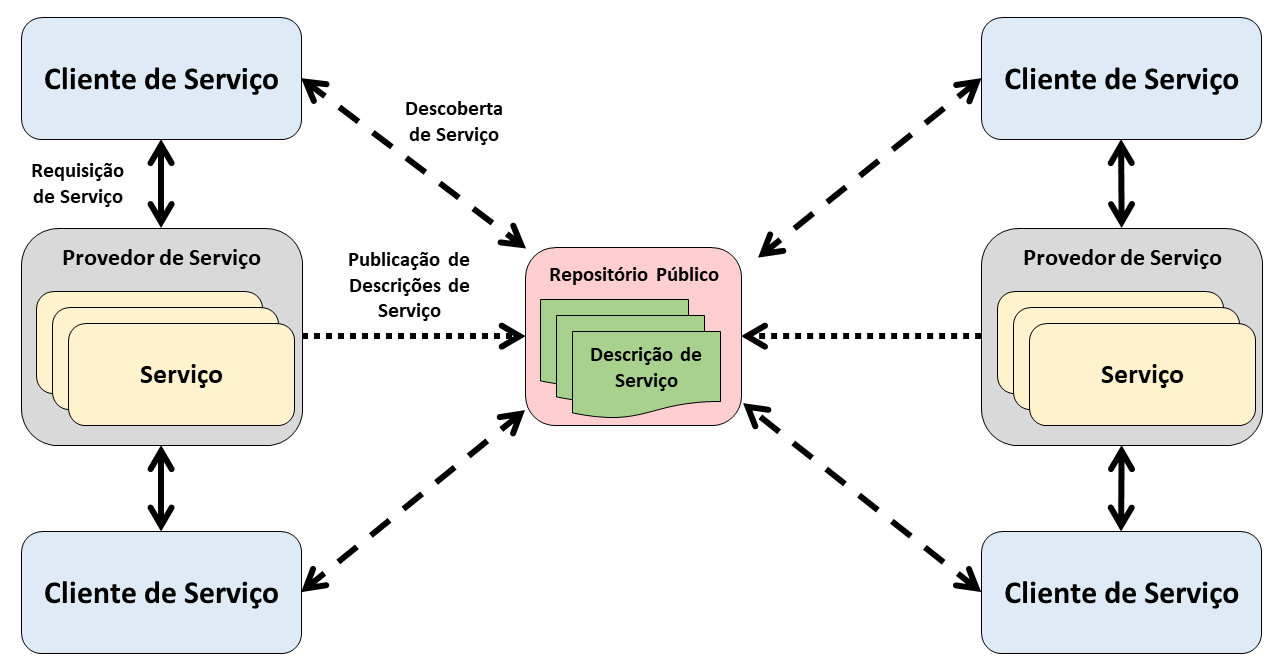
\includegraphics[scale=0.45]{2-fundamentacao-teorica/imagens/arquitetura-orientada-a-servicos(1).png}
    \centering
    \caption[Arquitetura orientada à serviços.]{\textbf{Arquitetura orientada a serviços.}}
    \label{fig:arquitetura-orientada-servicos}
\end{figure}
\subsection{Serviços Web}\label{2-fundamentacao-dbs-servicos-web}

Serviços web representam uma solução tecnológica concreta para o desenvolvimento baseado em serviços. Um serviço web utiliza um conjunto de padrões abertos da web para o seu desenvolvimento e invocação (utilização), sendo identificado univocamente por um \textit{Uniform Resource Identifier} (URI). Serviços web são atualmente desenvolvidos de acordo com duas principais abordagens: serviços SOAP e serviços RESTful.

\subsubsection{Serviços SOAP}\label{2-fundamentacao-dbs-servicos-web-soap}

Serviços web SOAP são implementados utilizando um conjunto de tecnologias e padrões abertos de desenvolvimento providos pela W3C~\cite{DACONTA-OBRST-SMITH-2003-The-Semantic-Web}. Os três principais padrões usados no desenvolvimento de serviços web SOAP são o protocolo \textit{Simple Object Access Protocol} (SOAP)~\cite{W3C-2007-SOAP}, a linguagem de descrição de serviços \textit{Web Service Description Language} (WSDL)~\cite{W3C-2007-WSDL} e o registro de serviços \textit{Universal Description Discovery and Integration} (UDDI)~\cite{OASIS-2004-UDDI}.

Interações entre um serviço web SOAP e um cliente de serviço ocorrem com a utilização do protocolo SOAP~\cite{W3C-2007-SOAP}. O protocolo SOAP serializa os dados (objetos) envolvidos em uma interação usando XML. A transferência desses objetos, contidos nas mensagens de requisições, por parte de um cliente, e de respostas, por parte de um provedor, é normalmente realizada por meio do protocolo \textit{Hypertext Transfer Protocol} (HTTP).

A informação contida em uma mensagem criada a partir dos objetos serializados é armazenada no elemento \textit{envelope}, o qual é formado por dois outros elementos: \textit{header} e \textit{body}. O elemento \textit{envelope} define o documento XML como uma mensagem SOAP. O elemento \textit{header} contém informações específicas da mensagem SOAP, como, por exemplo, o endereço de IP de origem. Apesar de ser opcional, o elemento \textit{header}, se presente, deve ser o primeiro elemento-filho de envelope. O elemento \textit{body} armazena as informações referentes à requisição, como o nome dos métodos e o objeto serializado que será enviado na comunicação.

A linguagem WSDL é utilizada para descrever as funcionalidades e a localização de um serviço web SOAP~\cite{W3C-2007-WSDL}. O desenvolvimento de uma especificação WSDL possibilita que um serviço web seja consumido por outras aplicações por meio da disponibilização da descrição dos métodos do serviço, dos seus parâmetros e dos seus valores de retorno. Informações adicionais sobre a linguagem WSDL podem ser encontradas na seção \ref{2-fundamentacao-dbs-servicos-web-descricao-servico-web} deste documento.

UDDI consiste de um padrão para o registro (publicação) e a busca (descoberta) de descrições de serviços web SOAP em um repositório da Internet~\cite{PAPAZOGLOU-GEORGAKOPOULOS-2003-Service-Oriented-Computing, OASIS-2004-UDDI}. A partir do registro UDDI de um serviço web, realizado por um provedor de serviços, um cliente de serviços pode pesquisar e descobrir este serviço web. Além de contribuir com a busca de serviços web a partir de suas descrições, o UDDI provê informações necessárias para que um serviço possa ser reutilizado por um cliente~\cite{OASIS-2004-UDDI}, tais como informações sobre a organização que desenvolveu o serviço web ou sobre as regras de negócio associadas.

Um registro UDDI é criado com base em alguns elementos de uma especificação WSDL. UDDI contém todos os metadados de um serviço web, incluindo uma referência para a descrição WSDL de um serviço e um conjunto de definições que habilita a invocação deste serviço. Um registro UDDI fornece uma interface única (padronizada) que facilita a classificação, a localização, a invocação e o gerenciamento de metadados de um serviço.

%Tais recursos facilitam, portanto, a reutilização de um serviço web e, consequentemente, o desenvolvimento baseado em serviços.

A \figurename~\ref{fig:soap} ilustra a utilização dos diferentes padrões no desenvolvimento e invocação de um serviço web SOAP. A seta pontilhada representa a publicação de uma descrição de serviço WSDL em um repositório UDDI, feita por um provedor de serviços. A seta tracejada representa a descoberta de um serviço web junto a um repositório UDDI feita por um cliente de serviço. Finalmente, a seta sólida representa a requisição de serviço SOAP realizada por um cliente de serviço.

%A seta tracejada e pontilhada, localizada no canto inferior da figura, entre o provedor de serviços e as descrições WSDL, representa uma publicação de descrições de serviço (WSDL) em um repositório UDDI, feita por um provedor de serviços. A seta tracejada, localizada  no canto direito da figura, entre o cliente de serviços e as descrições WSDL, representa uma descoberta de serviços web, por meio de descrições WSDL existentes em um repositório UDDI, feita por um cliente de serviços. A seta sólida, localizada no centro da figura, entre o cliente de serviços e o provedor de serviços, representa uma requisição SOAP, realizada por um cliente de serviços. Por fim, a seta pontilhada, localizada no centro da figura, entre o provedor de serviço e o cliente de serviços, representa uma resposta SOAP para a requisição antes realizada.

%O processo inicia-se com um provedor de serviço desenvolvendo um serviço web e publicando (registrando) este serviço em um repositório UDDI (caixa rosa no centro inferior da figura). Um provedor de serviço pode desenvolver e publicar diversos serviços. Por isso, podemos visualizar diversos serviços (caixas amarelas) dentro do provedor de serviço (caixa cinza, no canto inferior esquerdo da figura). No repositório UDDI, podemos encontrar diversas descrições de serviços que utilizam a linguagem WSDL (caixas verdes, no canto inferior direito da figura). A publicação de descrições de serviço em um repositório UDDI é representada pela seta tracejada e pontilhada (canto inferior da figura, entre o provedor de serviço e as descrições WSDL).

%Ainda conforme a Figura \ref{fig:soap}, o segundo passo é um cliente de serviços (caixa azul, no canto superior direito da figura) realizar a busca e a descoberta de serviços por meio do repositório UDDI. Esta descoberta está representada pela seta tracejada (canto direito da figura, entre o cliente de serviços e as descrições WSDL). O terceiro passo é o cliente de serviços sendo capaz de consumir este serviço (invocar) após a sua descoberta. O consumo é feito por meio de uma requisição SOAP, sendo realizada diretamente no provedor de serviços. Esta requisição SOAP está representada por uma seta sólida (centro da figura, entre o cliente de serviços e o provedor de serviço). Por fim, o serviço retorna uma resposta SOAP para a requisição SOAP ao cliente de serviço. Esta resposta está representada por uma seta pontilhada (centro da figura, entre o provedor de serviço e o cliente de serviços).

\begin{figure}[h]
    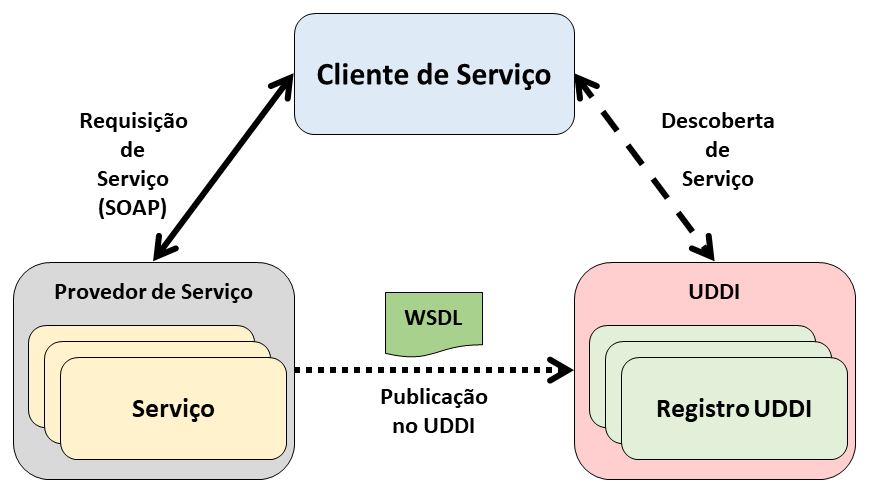
\includegraphics[scale=0.5]{2-fundamentacao-teorica/imagens/arquitetura-orientada-a-servicos(4).png}
    \centering
    \caption[Padrões abertos utilizados em um serviço web SOAP.]{\textbf{Padrões abertos utilizados em um serviço web SOAP.}}
    \label{fig:soap}
\end{figure}

\subsubsection{Serviços RESTful}\label{2-fundamentacao-dbs-servicos-web-restful}

REST (\textit{Representational State Transfer}) foi proposto como um modelo arquitetônico para guiar o projeto de desenvolvimento de sistemas computacionais distribuídos cujas interações entre as diferentes partes deste sistema são realizadas por meio do protocolo HTTP~\cite{FIELDING-2000-REST, CARDOSO-2006-Semantic-Web-Services}. REST é definido a partir de um conjunto de seis restrições arquitetônicas:

\begin{enumerate}

\item
\textit{Arquitetura Cliente-Servidor}, a qual separa a arquitetura de uma aplicação e as responsabilidades em duas partes, fazendo com que o cliente e o provedor não se preocupem com as atividades um do outro;

\item
\textit{Interações sem estado}, as quais definem que toda requisição contenha todas as informações necessárias para que o provedor consiga entendê-la e processá-la, sem a necessidade de informações adicionais ou providas por terceiros;

\item
\textit{Informações em cache}, as quais permitem que recursos muito requisitados por clientes possam ser armazenados, temporariamente, em cache, evitando processamento desnecessário e aumentando significativamente o desempenho;

\item
\textit{Interface uniforme}, a qual define um contrato para a comunicação entre clientes e provedores de serviços. Este contrato apresenta regras usadas para tornar um componente genérico, facilitando sua manutenção e expansão;

\item
\textit{Sistema em camadas}, o qual determina que o sistema seja estruturado em camadas hierárquicas, sendo que cada camada possui uma função específica. Essa estrutura possibilita que responsabilidades possam ser distribuídas entre as camadas, de modo que cada componente do sistema tenha papel e responsabilidades bem definidos;

\item
\textit{Código sob demanda}, o qual, apesar de ser opcional, permite que o cliente possa estender a parte lógica do provedor por meio de \textit{applets} e \textit{scripts}. Isso permite que diferentes clientes possam se comportar de maneiras diferentes, conforme suas necessidades, mesmo que consumam os mesmos serviços disponíveis no provedor.

\end{enumerate}

Os serviços criados com base no modelo arquitetônico REST são chamados de serviços RESTful. Estes serviços não são vinculados a uma tecnologia em particular, ou seja, podem ser desenvolvidos em qualquer plataforma ou linguagem de programação. Os serviços RESTful são mais simples de serem desenvolvidos do que os serviços SOAP, pois não impõem restrições quanto ao formato das mensagens trocadas entre as entidades envolvidas em uma interação. Tal característica permite que o desenvolvedor possa optar por um formato mais adequado para as mensagens do sistema de acordo com sua necessidade. Os formatos de mensagens mais comuns são JSON, XML e texto puro.

%A ausência formal de uma linguagem para descrever os serviços RESTful pode gerar problemas de interoperabilidade entre serviços e clientes. Embora não sejam obrigatórias, especificações da interface de um serviço podem ser criadas usando, por exemplo, a linguagem \textit{Web Application Description Language} (WADL)~\cite{W3C-2009-WADL}.

\subsubsection{Descrição de Serviços Web}\label{2-fundamentacao-dbs-servicos-web-descricao-servico-web}

%\hl{remover referencias de WSDL1.1 e simplificar o texto de WSDL2.0}

A descrição de um serviço web é composta por um conjunto de informações que definem como este serviço pode ser acessado. Tais informações incluem as operações disponíveis, os parâmetros e os valores de retorno, bem como a localização (endereço) do serviço.

Inicialmente, a linguagem \textit{Web Service Description Language} (WSDL) focou na especificação de serviços SOAP (até a versão 1.1 desta linguagem~\cite{W3C-2001-WSDL1.1}). Contudo, WSDL 1.1 não suportava a descrição de um serviço RESTful, pois não provia recursos suficientes para a descrição de todos os métodos HTTP possíveis de serem usados em um serviço RESTful. Assim, a versão 2.0 de WSDL~\cite{W3C-2007-WSDL} foi criada a fim de resolver tais restrições.

Outras abordagens, tais como \textit{Web Application Description Language} (WADL) \cite{W3C-2009-WADL} e \textit{OpenAPI}~\cite{SWAGGER-2017-OpenAPI-Specification}, podem ser utilizadas para a descrição de serviços RESTful. Porém, estas abordagens não são o foco deste trabalho.

%Dentre os problemas existentes, a versão 1.1 provia suporte apenas a serviços SOAP. A versão 2.0 da linguagem WSDL provê total suporte à descrições de serviços RESTful. Com isso, gostaríamos de ressaltar que o foco de interesse deste trabalho é na versão 2.0 do WSDL. Adicionalmente, um serviço RESTful pode ser descrito também por meio de \textit{Web Application Description Language} (WADL)~\cite{W3C-2009-WADL}.

%Atualmente, a especificação WSDL encontra-se na versão 2.0. Esta versão foi criada a fim de resolver problemas existentes de interoperabilidade contidos na versão 1.1. Dentre os problemas existentes, a versão 1.1 provia suporte apenas aos métodos GET e POST do protocolo HTTP. Já a versão 2.0 do WSDL tem total suporte para o protocolo HTTP. Esta versão passou a aceitar todos os métodos de requisições do HTTP – não apenas os métodos GET e POST, como na versão 1.1. Com isso, a descrição de serviços RESTful passou a ser suportada.

%Adicionalmente, WSDL 2.0 tem suporte à \textit{Internationalized Resource Identifiers} (IRIs). IRIs são um conjunto de URIs com suporte extra à internacionalização. Enquanto uma URI suporta apenas um conjunto limitado de caracteres do alfabeto inglês, números europeus e alguns símbolos, uma IRI permite usar caracteres de diversos alfabetos~\cite{W3C-2007-WSDL-Primer}.

%O WSDL 2.0 descreve um serviço da Web em dois estágios fundamentais: um abstrato e um concreto. Dentro de cada estágio, a descrição usa várias construções para promover a reutilização da descrição e separar as preocupações de design independentes.

A linguagem WSDL descreve um serviço web em duas partes fundamentais: parte abstrata e parte concreta. Dentro de cada parte, a descrição WSDL utiliza diferentes elementos que possibilitam a reutilização da descrição e também a separação de modelos independentes. A parte abstrata de uma descrição WSDL contém os elementos \textit{types}, \textit{operation} e \textit{interface}, enquanto que a parte concreta contém os elementos \textit{binding}, \textit{service} e \textit{endpoint}.

%Em um documento WSDL 2.0, há um conjunto simples de definições, composto por seis tipos de elementos: \textit{types}, \textit{operation} e \textit{interface}, que pertencem à parte abstrata da descrição; e \textit{binding}, \textit{service} e \textit{endpoint}, que pertencem à parte concreta da descrição. 

O elemento \textit{types} (\textit{<wsdl:types>}) representa os tipos de dados usados na comunicação. O elemento \textit{operation} (\textit{<wsdl:operation>}) representa uma descrição abstrata de uma ação (operação) suportada por um serviço, ou seja, representa uma funcionalidade suportada pelo serviço web. Adicionalmente, o elemento relaciona parâmetros de entrada (\textit{<wsdl:input>}) e de saída (\textit{<wsdl:output>}).

Operações (\textit{<wsdl:operation}>) são agrupadas por meio do elemento \textit{interface} (\textit{<wsdl:interface>}). Tal agrupamento tem por objetivo obter um formato padronizado para o transporte das mensagens. O elemento \textit{binding} (\textit{<wsdl:binding>}) especifica os detalhes do formato do transporte para uma ou mais interfaces. O elemento \textit{endpoint} (\textit{<wsdl:endpoint>}) associa um endereço de rede a um \textit{binding}. Finalmente, o elemento \textit{service} (\textit{<wsdl:service>}) agrupa os elementos \textit{endpoint}, a fim de implementar uma interface (\textit{<wsdl:interface>}) comum.

Falhas, também chamadas de exceções, consistem de comportamentos não esperados e não tratados no fluxo normal de execução de uma operação de um serviço. A ocorrência de falhas é representada por um elemento do tipo \textit{fault} (\textit{<wsdl:fault>}). O elemento \textit{fault} é especificado diretamente dentro do elemento \textit{interface}, no mesmo nível dos elementos \textit{operation}. Desta forma, uma mensagem de falha pode ser reutilizada por diferente operações. Os elementos \textit{infault} (\textit{<wsdl:infault>}) e \textit{outfault} (\textit{<wsdl:outfault>}) representam instâncias de falhas de entrada e saída, respectivamente, que podem ocorrer dentro de cada operação. Na ocorrência de uma falha, se esta estiver tratada pelo serviço, a mensagem de resposta (\textit{<wsdl:output>}) de uma operação é substituída pela mensagem da falha.

%A especificação WSDL 2.0 também provê um mecanismo genérico para descrever os tipos de operações por meio dos \textit{Message Exchange Patterns} (MEPs)~\cite{W3C-2002-Web-Service-Message-Exchange-Patterns}. Um MEP é um modelo que estabelece um padrão para a troca de mensagens entre serviços SOAP, por meio da definição da ordem em que mensagens referentes a uma mesma operação são trocadas~\cite{NITZSCHE-LESSEN-LEYMAN-2008-Message-Exchange-Patterns}.

%No WSDL 1.1 haviam apenas quatro tipos de operações: \textit{One-way}, que apresenta um \textit{endpoint} que apenas recebe uma mensagem; Request-response, que apresenta um \textit{endpoint} que recebe uma mensagem e envia uma mensagem correspondente; \textit{Solicit-response}, que apresenta um \textit{endpoint} que envia uma mensagem e recebe uma mensagem correspondente; e \textit{Notification}, que apresenta um \textit{endpoint} que apenas envia uma mensagem. Dessa forma, no WSDL 1.1, era necessário mesclar os quatro tipos de operações a fim de obter resultados desejados pelos serviços. Já o WSDL 2.0 provê um mecanismo genérico para descrever os tipos de operações por meio dos \textit{Message Exchange Patterns} (MEPs)~\cite{W3C-2002-Web-Service-Message-Exchange-Patterns}. Um MEP é um modelo que estabelece um padrão para a troca de mensagens entre serviços SOAP, por meio da definição da ordem em que mensagens referentes a uma mesma operação são trocadas~\cite{NITZSCHE-LESSEN-LEYMAN-2008-Message-Exchange-Patterns}.
\section{Serviços Web Semânticos}\label{2-fundamentacao-sws}

Esta seção apresenta uma visão geral acerca da representação de conhecimento por meio de ontologias OWL, introduz a definição de serviços web semânticos e, por fim, apresenta a abordagem SAWSDL para o desenvolvimento de serviços web semânticos.

\subsection{Representação do Conhecimento}\label{2-fundamentacao-sws-representacao-conhecimento}

O conhecimento de um dado domínio pode ser formalmente representado por meio de uma conceitualização~\cite{GRUBER-1993-Ontologies, GRUBER-1995-Ontologies}. Uma conceitualização consiste em definições de entidades (objetos) que presume-se existir em uma determinada área de conhecimento (interesse), incluindo as relações existentes entre estes objetos. Assim, uma conceitualização representa uma visão simplificada e abstrata de um domínio de conhecimento. Toda base de conhecimento, todo sistema baseado em conhecimento ou agente baseado em conhecimento estão relacionados à alguma conceitualização, de forma explícita ou implícita.

Uma ontologia representa uma especificação explícita de uma conceitualização. Na Filosofia, uma ontologia representa um relato sistemático da existência de objetos de um dado domínio. Quando o conhecimento de um domínio é representado por meio de um formalismo declarativo, o conjunto formado pelos conceitos que podem ser representados é chamado de universo de discurso~\cite{GRUBER-1993-Ontologies}.

%Este conjunto de objetos e relacionamentos são especificados para representar este universo de discurso.

Na área da computação, uma ontologia é um artefato criado para representar de forma explícita o conhecimento de um domínio por meio de definições de conceitos e relacionamentos entre os mesmos. Uma ontologia é geralmente desenvolvida por especialistas do domínio de interesse. Atividades como análises conceituais e modelagem de domínios com base em metodologias-padrões têm sido elaboradas ao longo dos anos com o objetivo de aprimorar e padronizar o desenvolvimento de novas ontologias~\cite{GUARINO-1998-Ontology}. O estudo de ontologias tem sua importância reconhecida nas áreas de Inteligência Artificial, Linguística Computacional, Teoria de Banco de Dados, entre outras.

Atualmente, um volume crescente de dados tem sido disponibilizado na Web. A Web Semântica tem por objetivo associar dados (documentos) disponíveis na Web a significados bem definidos~\cite{BERNERS-HENDLER-LASSILA-2001-Semantic-Web}. Esta associação facilita a recuperação de informações, a integração e o reuso destes dados, tanto por máquinas quanto por seres humanos~\cite{CARDOSO-2006-Semantic-Web-Services}. Para criar esta realidade, anotações semânticas devem ser adicionadas aos dados contidos em documentos HTML e XHTML da Web. As anotações semânticas são feitas a partir de referências a conceitos definidos em uma ontologia. 

Dentre as linguagens utilizadas para a representação de conhecimento, destaca-se a linguagem \textit{Web Ontology Language} (OWL), atualmente na versão 2.0~\cite{W3C-2012-OWL, W3C-2012-OWL-Primer}. OWL é uma linguagem para a construção de ontologias em diferentes domínios de conhecimento. O conhecimento em uma ontologia OWL é representado por meio da especificação de classes, propriedades, instâncias e valores. Uma ontologia OWL pode ser representada usando-se diferentes sintaxes, tais como \textit{Functional-Style}, RDF/XML, \textit{Manchester}, \textit{Turtle} e OWL/XML. A linguagem OWL faz parte de um conjunto de recursos da Web Semântica, que incluem RDF~\cite{W3C-2014-RDF}, RDFS~\cite{W3C-2007-RDFS}, SPARQL~\cite{W3C-2008-SPARQL}, entre outros.
\subsection{Definição de Serviços Web Semânticos}\label{2-fundamentacao-sws-definicao}

O Desenvolvimento Baseado em Serviços pressupõe o reuso e a integração de serviços (composição de serviços). Porém, como identificar se um serviço atende às necessidades (funcionais) de um dado cliente e como identificar e resolver eventuais problemas de incompatibilidade semântica de modo a obter a interoperabilidade desejada entre diferentes serviços? Para responder a tais questionamentos, são necessárias informações precisas sobre as funcionalidades de um determinado serviço, bem como sobre os dados de entrada e de saída deste serviço.

Serviços web semânticos (SWS) representam a extensão de serviços web com a aplicação dos princípios da Web Semântica. SWS representam serviços web cujas interfaces são semanticamente anotadas com conceitos (termos) definidos em uma ontologia. Neste sentido, SWS são criados a partir da adição de definições semânticas a interfaces de serviços web, bem como a operações e a dados de entrada e saída destas operações~\cite{CARDOSO-2006-Semantic-Web-Services, W3C-2007-SAWSDL, STAVROPOULOS-2013-Iridescent}.

O desenvolvimento de SWS proporciona diferentes benefícios, dentre os quais destacam-se~\cite{SHETH-2007-SAWSDL-Tools}: i) facilidade de reuso de serviços, dado que descrições semânticas colaboram para encontrar serviços mais relevantes; ii) interoperabilidade semântica, alcançada por meio da anotação e do mapeamento semântico realizado entre os dados trocados entre serviços web; iii) facilidade de configuração e composição, permitindo ligações dinâmicas entre diferentes serviços web; iv) e, por fim, nível mais elevado de automação no ciclo de vida de uma atividade desenvolvida por uma organização, ou seja, auxilia na configuração dinâmica (análises de descoberta e restrições) e execução (tratamento de exceções durante a execução) dos processos desenvolvidos por uma organização.
\subsection{Abordagem SAWSDL}\label{2-fundamentacao-sws-sawsdl}
%\subsubsection{SAWSDL}\label{2-fundamentacao-sws-abordagens-sawsdl}

\textit{Semantic Annotations for WSDL and XML Schema} (SAWSDL) é um formato padrão da W3C para anotações semânticas em documentos WSDL~\cite{W3C-2007-SAWSDL}. SAWSDL define mecanismos para permitir que anotações semânticas possam ser adicionadas em um documento WSDL a partir de conceitos contidos em uma ontologia. Assim, SAWSDL pode ser visto como um conector, associando descrições puramente sintáticas, representadas por serviços web e suas descrições, a conceitos semânticos, representados por ontologias~\cite{KOPECKY-VITVAR-BOURNEZ-FARREL-2007-SAWSDL}. A partir desta associação, aplicações computacionais podem interpretar (parcialmente ou completamente) esses conceitos, a fim de automatizar tarefas, tais como o descobrimento, a seleção e a composição de serviços web.

SAWSDL é independente de linguagens específicas para a representação de ontologias, bastando que os conceitos semânticos possam ser identificados a partir de URIs. Normalmente, os \textit{frameworks} de anotação semântica para serviços web utilizam OWL/RDF (\textit{Resource Description Framework}) em conjunto com SAWSDL. SAWSDL contém dois tipos de atributos: \textit{Model Reference} e \textit{Schema Mapping}. Ambos são apresentados a seguir.

Um atributo \textit{Model Reference} (\textit{sawsdl:modelReference}) representa uma anotação de um elemento (entidade) de um documento WSDL com referências a um conjunto de conceitos definidos em uma ou mais ontologias~\cite{KOPECKY-VITVAR-BOURNEZ-FARREL-2007-SAWSDL}. O valor contido no atributo \textit{Model Reference} é um conjunto de zero ou mais URIs, separados por espaços, que identificam, cada qual um diferente conceito~\cite{W3C-2007-SAWSDL}. Dada a definição de uma interface WSDL, o atributo \textit{Model Reference} pode ser utilizado para prover uma descrição semântica para a interface (\textit{<wsdl:interface>}) como um todo e/ou para cada operação (\textit{<wsdl:operation>}) definida nesta interface.

Embora os nomes dos elementos de entrada e de saída possam indicar o comportamento esperado de uma operação, tal objetivo nem sempre pode ser atingido dada a possível incerteza e ambiguidade intrínseca aos identificadores utilizados. Neste sentido, cada elemento de uma entrada, saída ou falha associado a cada operação definida pode ser individualmente anotado com o atributo modelReference para prover uma descrição semântica para este elemento. A anotação de uma falha é composta por uma referência a um conceito semântico que provê uma descrição geral (alto nível) da falha. A anotação da ocorrência de uma falha não descreve a mensagem da falha em si. Esta mensagem deve ser criada como um elemento XSD, do documento \textit{XML Schema}, e, portanto, este elemento também pode ser anotado. 

O atributo \textit{Model Reference} também pode ser utilizado para anotar os elementos pertencentes ao documento \textit{XML Schema} (XSD), como, por exemplo, \textit{<xs:element>}, \textit{<xs:attribute>}, \textit{<xs:simpleType>} e \textit{<xs:complexType>}. Os elementos \textit{<xs:element>} e \textit{<xs:attribute>} podem ser anotados com \textit{Model Reference}, com o propósito de descrever um conceito definido em um modelo semântico. Ao anotar um elemento \textit{<xs:simpleType>}, qualquer elemento ou atributo deste tipo simples também será associado ao conceito do modelo semântico referenciado.

Um elemento \textit{<xs:complexType>} pode ser anotado segundo duas abordagens distintas: \textit{Bottom Level Annotation} e \textit{Top Level Annotation}. \textit{Bottom Level Annotation} refere-se à anotação aplicada a um elemento, que compõe o tipo complexo, ou a um atributo. Deste modo, todos os elementos e atributos de um tipo complexo podem ser anotados, caracterizando, portanto, uma anotação mais granularizada e específica para os elementos-filhos. Já \textit{Top Level Annotation} refere se à anotação do elemento complexo como um todo, caracterizando, portanto, uma anotação mais genérica, sem se especializar nos elementos e atributos contidos no compartimento-pai. Apesar da existência de duas abordagens, elas são independentes, podendo ser utilizadas simultaneamente em um elemento \textit{<xs:complexType>} (\textit{Top Level Annotation}) e seus elementos-filhos (\textit{Bottom Level Annotation}).

Um atributo do tipo \textit{Schema Mapping} é utilizado para tratar eventuais incompatibilidades existentes entre o modelo semântico (ontologia) e a estrutura de parâmetros de entrada (\textit{input}) e saída (\textit{output}) de um serviço web (WSDL). O atributo \textit{Schema Mapping} permite que transformações (conversões) de tipos de dados contidos em um serviço web e em uma ontologia sejam realizadas por meio de métodos \textit{Lifting} e \textit{Lowering}.

O método \textit{Lifting}, representado pelo atributo \textit{sawsdl:liftingSchemaMapping}, permite que dados presentes em um nível sintático (WSDL/XML) sejam mapeados para um nível semântico. Neste sentido, \textit{Lifting} permite que dados no formato XML, produzidos por um serviço web, sejam transformados em instâncias de um modelo semântico, como, por exemplo, instâncias de classes OWL. O método \textit{Lowering}, representado pelo atributo \textit{sawsdl:loweringSchemaMapping}, permite que dados possam ser manipulados de forma ontológica, i.e., \textit{Lowering} transforma os tipos de dados de um nível semântico em tipos de dados de um nível sintático (WSDL/XML). Neste sentido, \textit{Lowering} permite que instâncias de classes OWL possam ser transformadas de volta em dados no formato XML.

Cabe ressaltar que o SAWSDL não especifica a forma como a transformação dos dados sintáticos para os semânticos (ou vice-versa) será realizada. Os atributos \textit{sawsdl:liftingSchemaMapping} e \textit{sawsdl:loweringSchemaMapping} apenas fazem referência a um URI contendo um conjunto de regras de transformação. Estas regras podem ser definidas usando, por exemplo, as linguagens \textit{EXtensible Stylesheet Language Transformation} (XSLT)~\cite{W3C-1999-XSLT} e XQuery~\cite{W3C-2017-XQuery}.
%\input{2-fundamentacao-teorica/2.2.4-owl-s}
%\input{2-fundamentacao-teorica/2.2.5-wsmo-lite}
\section{Notação Visual}\label{2-fundamentacao-notacao-visual}

Esta seção apresenta uma visão geral acerca de um conjunto de princípios associados ao desenvolvimento de notações visuais.

\subsection{Visão Geral}\label{2-fundamentacao-notacao-visual-visao-geral}

Notações visuais são uma das formas mais antigas e efetivas de representação do conhecimento~\cite{DAVIES-1990-Egyptian-Hieroglyphs, MATHEWS-Classic-1991-Maya_Emblem_Glyphs, KAMESWARA-2005-Prehistoric-Astronomy-India}. Diferentes tipos de recursos visuais, tais como formas geométricas, cores, ícones, texturas e brilhos, podem ser utilizados para representar diferentes conceitos e seus relacionamentos em um dado domínio~\cite{SMITH-MORIARTY-KENNEY-BARBATSIS-2004-Handbook-Visual-Communication, MOODY-2009-Physics-Notation}.

Notações visuais são mais eficazes para a comunicação e a transmissão de informações do que outras formas de comunicação, incluindo a comunicação verbal e textual~\cite{MOODY-2009-Physics-Notation}. Tal característica advém da melhor capacidade do cérebro humano em processar (paralelamente) representações visuais, que utilizam arranjos espaciais de elementos gráficos (bidimensionais). Cerca de um quarto do cérebro humano é dedicado à visão. Assim, o sistema visual de um cérebro humano tem a capacidade de processar mais informações do que todos os demais sentidos combinados.

%Por outro lado, o processamento de notações textuais não é tão eficaz, dado que notações textuais utilizam sequências de caracteres para representações unidimensionais (lineares) e são processadas em série pelo cérebro humano.

%Adicionalmente, o cérebro humano possui sistemas separados com diferentes propósitos, como, por exemplo, o sistema visual para o processamento de representações visuais e o sistema auditivo para o processamento de representações verbais. Cerca de um quarto do cérebro humano é dedicado à visão. O sistema visual de um cérebro humano tem a capacidade de processar mais informações do que todos os demais sentidos combinados.

Atualmente, notações visuais tem sido amplamente utilizadas em diversas áreas de conhecimento. Por exemplo, \textit{Unified Modeling Language} (UML)~\cite{OMG-2017-UML} tem sido utilizada na representação de artefatos de \textit{software}; \textit{Business Process Management Notation} (BMPN)~\cite{OMG-2011-BPMN} tem sido utilizada na representação de processos de negócio; \textit{Systems Biology Graphical Notation} (SBGN)~\cite{NOVERE-BUCKA-MI-MOODIE-SCHREIBER-SOROKIN-2009-SBGN, VASUNDRA-LENOVERE-WALTEMATH-WOLKENHAUER-2018-SBGN} tem sido utilizada na representação de modelos biológicos \textit{in silico}; enquanto que \textit{Synthetic Biology Open Language} (SBOL)~\cite{QUINN-COX-ADLER-2015-SBOL} tem sido utilizada na representação de modelos de engenharia genética.
\subsection{Princípios da Notação Visual}\label{2-fundamentacao-notacao-visual-principios}

Historicamente, pesquisadores e projetistas de notações visuais ignoraram ou subestimaram princípios básicos da sintaxe para representar visualmente elementos de um modelo~\cite{MOODY-2009-Physics-Notation}. O desenvolvimento das notações visuais existentes em diversas áreas de conhecimento, como na engenharia de \textit{software}, foi, em sua maioria, visando atender apenas a detalhes semânticos, pouco atentando a convenções visuais.

De modo a projetar notações visuais cognitivamente eficazes, otimizando, portanto, o suporte à comunicação humana e à solução de problemas, Moody propôs um conjunto de nove princípios, chamados de Física das Notações~\cite{MOODY-2009-Physics-Notation}. Estes princípios tem como base a representação visual de constructos~\cite{MOODY-2009-Physics-Notation, POPESCU-WEGMANN-2014-Using-Physics-of-Notation-SEAM}. Constructos são modelos criados mentalmente e usados por especialistas para compreender uma parte específica de um domínio ou teoria. Construções mentais ou sínteses feitas a partir da combinação de vários elementos contribuem para a definição de um constructo. Tais construções mentais têm por objetivo a compreensão da realidade que deriva das observações e percepções individuais, resultantes de experiências (passadas ou presentes) de uma pessoa.

Os princípios da Física das Notações concentram-se nas propriedades físicas de uma notação (perceptivo) em vez de suas propriedades lógicas (semânticas). Eles foram sintetizados a partir de evidências empíricas de uma ampla variedade de domínios e baseiam-se em uma teoria explícita de como as notações visuais se comunicam. Esses princípios podem ser usados para construir novas notações visuais, bem como para avaliar, comparar e melhorar as notações visuais existentes. Cada princípio é independente dos demais, podendo ser aplicados separadamente.

\subsubsection{Princípio da Integração Cognitiva}\label{2-fundamentacao-notacao-visual-principio-integracao-cognitiva}

Notações visuais devem ter informações (representações) integradas entre diferentes modelos. Ou seja, se um elemento é representado em dois modelos distintos, este elemento deve possuir a mesma representação visual em ambos os modelos. Este princípio apenas se aplica quando múltiplos modelos são usados. Os modelos podem ser do mesmo tipo (integração homogênea) ou de tipos diferentes (integração heterogênea). Mecanismos de integração cognitiva referem-se a integrações conceituais (sumarização e momento visual) e integrações perceptivas (sinalização, orientação e mapa de navegação).

\subsubsection{Princípio do Ajuste Cognitivo}\label{2-fundamentacao-notacao-visual-principio-ajuste-cognitivo}

Notações visuais devem ter diferentes dialetos para diferenciar a comunicação entre diferentes públicos-alvos (audiência). O público-alvo pode ser composto por especialistas ou por iniciantes em um dado domínio. Diferentes dialetos visuais também podem ser necessários para diferentes objetivos (tarefas). Notações cognitivamente eficazes para uma audiência iniciante podem não ser cognitivamente eficazes para uma audiência de especialistas e vice-versa. O princípio do ajuste cognitivo afirma, portanto, que variações de uma mesma notação visual são necessárias e devem ser utilizadas conforme a audiência e os diferentes objetivos que pretende-se atingir com o uso de um dado modelo.

\subsubsection{Princípio da Diferenciação Perceptiva}\label{2-fundamentacao-notacao-visual-principio-diferenciacao-perceptiva}

Notações visuais devem ser claramente distinguíveis umas das outras. Esta distinção pode ser obtida aumentando as diferenças visuais entre as notações. Características como tamanho, forma e cor (expressividade visual) contribuem efetivamente na distinção de elementos visuais. Neste sentido, diferentes constructos semânticos devem ser facilmente identificados de acordo com suas diferentes (distintas) notações visuais. Informações textuais (codificação dupla) também podem ser utilizadas a fim de facilitar esta distinção.

\subsubsection{Princípio da Complexidade Gerenciável}\label{2-fundamentacao-notacao-visual-principio-complexidade-gerenciavel}

Modelos podem se tornar bastante complexos, dependendo diretamente da complexidade dos domínios em que eles estão sendo utilizados e do conhecimento que pretende ser representado~\cite{MOODY-2009-Physics-Notation}. Esta complexidade diagramática pode também ser medida pela quantidade de elementos visuais de um modelo. Quanto mais detalhada e granular a representação visual de um conhecimento, maior é a complexidade de um modelo. Neste sentido, notações visuais devem incluir mecanismos explícitos para lidar com modelos complexos, como, por exemplo, por meio da divisão destes em sub-modelos.

A complexidade pode também ser tratada por meio da modularização de um modelo complexo. A modularização envolve tanto a criação de modelos mais genéricos (com menos detalhes), de modo a obter uma visão mais abstrata do modelo, quanto a criação de modelos mais específicos (com mais detalhes), de modo a obter uma visão mais concreta e realista do modelo em desenvolvimento.

%A divisão de um modelo, realizada por meio da modularização e da divisão de uma estrutura hierárquica, possibilita a criação, portanto, de modelos mais genéricos (com menos detalhes) e de modelos mais específicos (com mais detalhes). Modularização refere-se a ter modelos mais genéricos, estes a fim de obter-se uma visão generalizada (simplista) do modelo, e modelos mais específicos, contendo um maior nível de granularidade e detalhes, a fim de obter-se uma visão especializada em um dado contexto do modelo que pretende-se representar visualmente.

\subsubsection{Princípio da Clareza Semiótica}\label{2-fundamentacao-notacao-visual-principio-clareza-semiotica}

O princípio da clareza semiótica relata que um constructo semântico (conceito) deve ser representado por exatamente um elemento gráfico (visual) e vice-versa~\cite{MOODY-2009-Physics-Notation}. Ou seja, deve haver uma relação 1:1 (um-para-um) entre constructos semânticos e notações visuais.

Há quatro formas de violação deste princípio, chamadas de anomalias da clareza semiótica: i) redundância de símbolos, i.e., um constructo semântico é representado por várias notações visuais; ii) sobrecarga de símbolos, i.e., uma notação visual representa mais de um constructo semântico; iii) excesso de símbolos, i.e., a notação visual é criada e não representa qualquer constructo semântico; e, por fim, iv) carência de símbolos, i.e., não há nenhuma notação visual prevista para um certo constructo semântico.

A \figurename~\ref{elementofig:anomalias-clareza-semiotica} resume as quatro anomalias da clareza semiótica. Os elementos \texttt{C\textsubscript{i}}, à esquerda, representam constructos semânticos, enquanto que os elementos \texttt{S\textsubscript{i}}, à direita, representam símbolos.

%O elemento \texttt{C\textsubscript{1}} não possui uma representação visual. Portanto, \texttt{C\textsubscript{1}} caracteriza-se pela anomalia de carência de elementos. O elemento \texttt{C\textsubscript{2}} possui duas representações visuais: \texttt{S\textsubscript{1}} e \texttt{S\textsubscript{2}}. Portanto, \texttt{C\textsubscript{2}} caracteriza-se pela anomalia de redundância de elementos. \texttt{C\textsubscript{3}} e \texttt{C\textsubscript{4}} compartilham da mesma representação visual: \texttt{S\textsubscript{3}}. Portanto, \texttt{C\textsubscript{3}} e \texttt{C\textsubscript{4}} caracterizam-se pela anomalia de sobrecarga de símbolos. Finalmente, \texttt{S\textsubscript{4}} é uma representação visual que não possui um constructo semântico relacionado. Portanto, \texttt{S\textsubscript{4}} caracteriza-se pela anomalia de excesso de símbolos.

\begin{figure}[h]
    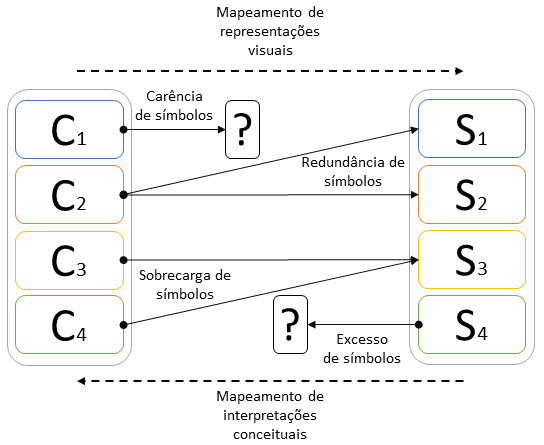
\includegraphics[scale=0.8]{2-fundamentacao-teorica/imagens/clareza-semiotica.png}
    \centering
    \caption[Anomalias do princípio da clareza semiótica.]{\textbf{Anomalias do princípio da clareza semiótica.} Adaptado de~\cite{MOODY-2009-Physics-Notation}}
    \label{elementofig:anomalias-clareza-semiotica}
\end{figure}

\subsubsection{Princípio da Expressividade Visual}\label{2-fundamentacao-notacao-visual-principio-expressividade-visal}

Notações visuais podem fazer uso de sete diferente variáveis visuais para melhorar a expressividade de uma notação visual: posição, tamanho, brilho, textura, cor, orientação e forma. A expressividade visual é determinada pelo número de variáveis visuais usadas em uma notação e a extensão em que elas são utilizadas. Porém, no contexto do nosso trabalho, as variáveis cor, tamanho, forma e posição são consideradas mais relevantes.

A cor é uma das mais importantes variáveis visuais, uma vez que o contraste de cor é interpretado mais rapidamente do que as diferenças entre outras variáveis. Porém, cores devem ser usadas com cuidado e apenas em conjunto (de forma redundante) com outras variáveis, dado que suas diferenças desaparecem quando modelos são impressos em escala de cinza ou então quando os modelos são utilizados por pessoas daltônicas.

Elementos visuais também podem ser diferenciados pelo uso de diferentes formas e tamanhos. Por exemplo, retângulos podem ser utilizados para representar atividades enquanto losangos podem ser utilizados para representar decisões na BPMN~\cite{OMG-2011-BPMN}. Em um modelo de nuvem de palavras~\cite{HEIMER-LOHMANN-LANGE-ERTL-2014-WORD-CLOUD}, o tamanho de uma dada palavra-chave é proporcional à relevância desta no modelo. Quanto mais revelante, maior é a palavra em relação às demais.

%Para diferentes tamanhos, como exemplo, podemos citar elementos mais importantes (mais relevantes) podem ter tamanhos maiores em relação à elementos menos importantes em um modelo, como é o exemplo de palavras-chave mais relevantes um dado contexto sendo representadas com tamanhos maiores em um modelo de nuvem de palavras~\cite{HEIMER-LOHMANN-LANGE-ERTL-2014-WORD-CLOUD}.

Elementos visuais podem ser diferenciados conforme o seu posicionamento, ou seja, conforme a sua posição no eixo X (horizontal) e no eixo Y (vertical). Por exemplo, em um organograma empresarial, profissionais líderes podem ser apresentados verticalmente (eixo Y) acima de seu time, bem como profissionais com o mesmo cargo podem ser apresentados no mesmo nível vertical (eixo Y), porém espaçados (distribuídos) horizontalmente (eixo X).

Diferentes brilhos e texturas também podem contribuir para uma maior expressividade visual. O brilho pode alterar a tonalidade de uma representação visual e muitas vezes é utilizado em conjunto com as cores a fim de se obter uma maior diferenciação entre elementos de um modelo. Por fim, orientações de notações visuais, como diferentes ângulos (rotações) utilizados para um mesmo elemento visual, podem contribuir para representar diferentes conceitos semânticos em um dado modelo.

\subsubsection{Princípio da Economia Gráfica}\label{2-fundamentacao-notacao-visual-principio-economia-grafica}

Notações visuais devem ser utilizadas com parcimônia, ou seja, o número de elementos gráficos deve ser limitado e de fácil gerenciamento. Um grande número de convenções aumenta a complexidade de um modelo, dificultando o seu entendimento.

A fim de satisfazer o princípio da economia gráfica, três abordagens podem ser utilizadas. A primeira abordagem refere-se à remoção de constructos semânticos, ou seja, reduz-se a quantidade de constructos semânticos e, consequentemente, de representações visuais relacionadas. Esta redução deve ser realizada com cuidado a fim de que o princípio clareza semiótica não venha a ser violado. A segunda abordagem refere-se à simples eliminação de representações visuais. Contudo, esta abordagem é mais arriscada, visto que a anomalia carência de símbolos, da clareza semiótica, pode ser mais facilmente introduzida. Por fim, a terceira abordagem refere-se ao aumento da expressividade visual. Esta abordagem pressupõe que com o aumento de características (atributos) visuais de um dado elemento, enriquecendo, portanto, a sua expressividade visual, este elemento pode ser tornar suficientemente claro para substituir simultaneamente dois ou mais elementos em um dado modelo.

\subsubsection{Princípio da Codificação Dupla}\label{2-fundamentacao-notacao-visual-principio-codificacao-dupla}

Textos contribuem para a compreensão de um modelo quando usados em conjunto com representações gráficas. Assim, notações visuais devem utilizar tanto elementos gráficos quanto elementos textuais. Uma representação textual não deve substituir uma representação gráfica, mas sim complementá-la. O uso de elementos textuais com elementos gráficos contribui para uma transmissão de informação mais efetiva do que quando usados de forma separada. Entretanto, é importante que as representações gráficas sejam distinguíveis com base nas ilustrações. Elementos como rótulos (\textit{labels}) devem ser utilizados apenas para distinguir instâncias de um mesma representação gráfica, mas não entre tipos (elementos) diferentes.

\subsubsection{Princípio da Transparência Semântica}\label{2-fundamentacao-notacao-visual-principio-transparencia-semantica}

Notações visuais devem utilizar elementos gráficos cuja aparência sugerem o significado de seus constructos semânticos. Transparência semântica avalia a facilidade com a qual uma representação visual é relacionada ao seu real significado (constructo).

A transparência semântica de um elemento pode ser classificada em: semanticamente imediata, semanticamente opaca ou semanticamente perversa. Um elemento é semanticamente imediato se um leitor iniciante é capaz de inferir o seu significado por si só a partir da sua aparência. Por exemplo, um boneco para representar uma pessoa. Um elemento é semanticamente opaco (ou convencional) se existe uma relação puramente arbitrária entre a sua aparência e seu significado. Por exemplo, um retângulo para representar uma entidade em um diagrama entidade relacionamento (DER). Finalmente, um elemento é semanticamente perverso (ou um falso mnemônico), se um leitor iniciante é susceptível a inferir um significado diferente ou até mesmo oposto ao significado do elemento. Por exemplo, uma classe pode ser interpretada como uma interface em um diagrama de classes da UML.

Uma abordagem eficaz de se modelar elementos com transparência semântica é por meio de ícones. Ícones facilitam o reconhecimento de constructos semânticos. Adicionalmente, ícones melhoram a compreensão da notação principalmente para os usuários iniciantes. Notações visuais semanticamente transparentes também reduzem a carga cognitiva, visto que elas têm mnemônicos embutidos e o seu significado pode ser percebido diretamente ou facilmente aprendido.

A \figurename~\ref{fig:transparencia-semantica} ilustra as medidas da transparência semântica. Quanto mais à direita (sinal positivo), mais um elemento visual é semanticamente imediato. Quanto à esquerda (sinal negativo), mais um elemento visual é semanticamente perverso. No centro do eixo, entre semanticamente imediato e semanticamente perverso, um elemento pode ser considerado semanticamente opaco (neutro).

\begin{figure}[h]
    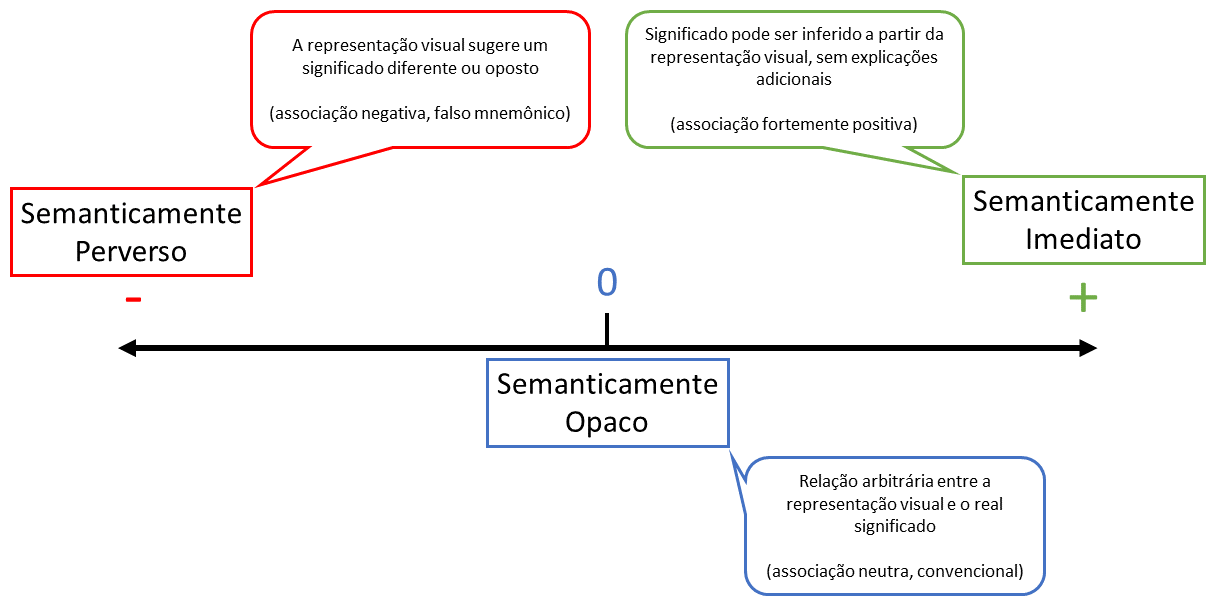
\includegraphics[scale=0.48]{2-fundamentacao-teorica/imagens/transparencia-semantica.png}
    \centering
    \caption[Princípio da transparência semântica.]{\textbf{Princípio da transparência semântica.} Adaptado de~\cite{MOODY-2009-Physics-Notation}}
    \label{fig:transparencia-semantica}
\end{figure}
\section{Sistemas Colaborativos}\label{2-fundamentacao-sistemas-colaborativos}

Esta seção apresenta uma introdução a sistemas colaborativos, com foco na edição colaborativa de documentos.

%por fim, de algumas ferramentas de suporte à edição colaborativa de documentos.

\subsection{Visão Geral}\label{2-fundamentacao-sistemas-colaborativos-visao-geral}

Uma sociedade muitas vezes é caracterizada pela forma com a qual seus indivíduos se interagem~\cite{ELLIS-GIBBS-REIN-1991-Sistemas-Colaborativos}. O uso de computadores e outros dispositivos eletrônicos de comunicação, presentes tanto em ambientes organizacionais quanto em residenciais, contribuem para o surgimento de novas formas de interação. Uma interação pode ser classificada conforme sua relação com as dimensões do espaço e do tempo. Em relação ao tempo, uma interação pode ser realizada ao mesmo tempo (síncrona) ou em tempos diferentes (assíncrona). Em relação ao espaço, um interação pode ser realizada no mesmo local ou em diferentes locais. A \tablename~\ref{tab:formas-interacao-espaco-tempo} apresenta uma matriz de classificação das formas de interação entre espaço e tempo.

\begin{table}[ht!]
    \setlength{\tabcolsep}{10pt} % Default value: 6pt
    \renewcommand{\arraystretch}{1.5} % Default value: 1
    \centering
    \caption[Classificação das formas de interação em relação ao tempo e ao espaço.]{\textbf{Classificação das formas de interação em relação ao tempo e ao espaço.} Adaptado de~\cite{ELLIS-GIBBS-REIN-1991-Sistemas-Colaborativos}}.
    \label{tab:formas-interacao-espaco-tempo}
	%\resizebox{\textwidth}{!}{
		\begin{tabular}{ | g | c | c | }
			\hline
            \rowcolor{Gray}
			{} & \textbf{Mesmo tempo} & \textbf{Tempos diferentes}
			\\
			\hline
			\textbf{No mesmo local} & {Interação presencial} & {Interação assíncrona}
			\\
			\hline
			{} & {Interação síncrona} & {Interação assíncrona}
			\\
			\multirow{-1.5}{*}[3px]{\textbf{Em locais diferentes}} & {distribuída} & {distribuída}
			\\
            \hline
		\end{tabular}
	%}
\end{table}

Uma interação também pode ser classificada conforme os indivíduos presentes na interação (atores). Os atores podem ser tanto seres humanos (usuários) quanto máquinas (computadores e outros dispositivos eletrônicos). Atores podem interagir entre si por meio de diferentes formas. A \tablename~\ref{tab:formas-interacao-atores} apresenta uma matriz de classificação das formas de interação entre diferentes tipos de atores envolvidos.

\begin{table}[h]
    \setlength{\tabcolsep}{10pt} % Default value: 6pt
    \renewcommand{\arraystretch}{2} % Default value: 1
    \centering
    \caption[Classificação das formas de interação em relação aos atores.]{\textbf{Classificação das formas de interação em relação aos atores.}}
    \label{tab:formas-interacao-atores}
    %\resizebox{\textwidth}{!}{
        \begin{tabular}{ | g | c | c | }
            \hline
            \rowcolor{Gray}
            \textbf{} & \textbf{Usuário} & \textbf{Máquina}
            \\ \hline
            \textbf{Usuário} & {Interação usuário-usuário} & {Interação usuário-máquina}
            \\ \hline
            \textbf{Máquina} & {Interação usuário-máquina} & {Interação máquina-máquina}
            \\ \hline
        \end{tabular}
    %}
\end{table}

Interações do tipo usuário-usuário podem ser realizadas entre um grupo de dois ou mais usuários. A interação entre um grupo de usuários contribui para o trabalho em grupo, também chamado de trabalho colaborativo. O trabalho colaborativo tem se tornado cada vez mais essencial em atividades de uma organização~\cite{ELLIS-GIBBS-REIN-1991-Sistemas-Colaborativos}. Contudo, a maioria dos sistemas computacionais suportam interações apenas entre seus usuários e o sistema em si (interações do tipo usuário-máquina). Tarefas comuns como a edição de um documento de texto ou a escrita de um código-fonte de \textit{software} são geralmente realizadas de forma individual, tendo o envolvimento apenas de um único usuário (ser humano) e seu computador (máquina). Mesmo sistemas modelados para serem utilizados por multi-usuários proveem baixo suporte para interações de usuários com usuários (interações do tipo usuário-usuário). Este tipo de suporte é claramente necessário a fim de obter uma maior eficiência na realização de uma tarefa.

%A fim de atender às necessidades de suporte à interações de grupos, deve-se atender à três requisitos: comunicação, colaboração e coordenação.
%\textbf{Comunicação}
%\textbf{Colaboração}
%\textbf{Coordenação}
%Com o propósito de ser ter uma comunicação e colaboração efetiva, é necessário coordenar atividades realizadas por um grupo.

%\subsection{Trabalho Cooperativo Suportado por Computadores}\label{2-fundamentacao-sistemas-colaborativos-tcsc}

Trabalho Cooperativo Suportado por Computador (TCSC), do inglês \textit{Computer-Supported Cooperative Work} (CSCW), é uma área de estudo da computação. TCSC tem por objetivo investigar formas colaborativas com as quais grupos de trabalho realizam suas tarefas e como dispositivos computacionais podem auxiliar na realização destas tarefas. Sistemas computacionais que suportam a realização de tarefas por um grupo de pessoas com um mesmo objetivo são chamados de \textit{groupware}. Sistemas colaborativos que suportam interações simultâneas são chamados de  \textit{groupwares} de tempo real (\textit{groupwares} síncronos). Enquanto que sistemas colaborativos que suportam interações realizadas de forma não simultânea são chamados de  \textit{groupwares} assíncronos.

%Diversos sistemas computacionais que suportam o trabalho colaborativo estão disponíveis para as mais variadas tarefas, como, por exemplo, a edição colaborativa de documentos de texto ou a edição colaborativa de códigos-fonte de softwares.

Edição colaborativa refere-se à edição de um documento sendo realizada por mais de um usuário~\cite{DILLON-1993-Collaborative-Writing}. A edição colaborativa deve ser realizada com base em objetivo compartilhado entre as pessoas de um grupo. Cada pessoa realiza a sua contribuição individual a fim de atingir o objetivo de forma coletiva. Escolhas efetivas na conscientização, participação e coordenação do grupo são atividades críticas para o sucesso dos resultados obtidos pela escrita colaborativa~\cite{LOWRY-CURTIS-Taxonomy-2004-Collaborative_Writing}.

%\textit{Groupwares} devem prover  uma interface para um ambiente de trabalho compartilhado. Objetivos únicos e ambientes compartilhados são conceitos são cruciais que devem ser providos por \textit{groupwares}, de forma clara e com fácil compreensão pelos seus usuários.
\subsection{Desenvolvimento Colaborativo de Software}\label{2-fundamentacao-sistemas-colaborativos-desenvolvimento}

Sistemas computacionais tornaram-se vitais para a sociedade contemporânea~\cite{SOUZA-MARCZAK-PRIKLANDNICKI-2012-Desenvolvimento-Colaborativo-Software}. Diferentes organizações e negócios estão cada vez mais dependentes de funcionalidades fornecidas por estes sistemas, os quais têm se tornado cada vez mais complexos. A fim de atender aos desafios impostos por este aumento de complexidade, equipe de profissionais normalmente trabalham em conjunto no desenvolvimento de sistemas computacionais complexos. Estes profissionais trabalham colaborativamente para produzir soluções com sucesso, i.e., com qualidade, eficiência e eficácia. Entre estes especialistas, alguns papéis podem ser citados, como desenvolvedores, analistas de requisitos, arquitetos de \textit{softwares}, analistas de negócio, gerentes de projetos, entre outros. Os membros de uma equipe de desenvolvimento de \textit{software} precisam coordenar suas atividades, planejar novas ações, tomar decisões, realizar as atividades previstas e, também, comunicar-se com os demais membros da equipe.

O desenvolvimento de um sistema computacional requer a criação (colaborativa) de diferentes tipos de artefatos, tais como a especificação (textual) de requisitos do sistema, diagramas de casos de uso e de classe UML, e o código-fonte do sistema em uma dada linguagem de programação. Mudanças em quaisquer destes artefatos devem ser alinhadas (sincronizadas) corretamente de modo a evitar erros na interpretação, construção e execução deste sistema computacional.

Diversas ferramentas de desenvolvimento de \textit{software} dão suporte à colaboração entre os profissionais envolvidos no processo de desenvolvimento. Estas ferramentas dão suporte desde a especificação colaborativa de requisitos até a construção de diagramas e códigos-fonte. O suporte pode ocorrer de maneira síncrona ou assíncrona, passando por editores colaborativos de texto, que possibilitam que diferentes desenvolvedores de \textit{software} escrevam o código-fonte ao mesmo tempo, até sistemas que possibilitam gerenciar o acesso compartilhado de artefatos computacionais entre um determinado grupo de usuários (profissionais).

Durante o processo de edição colaborativa de um documento qualquer, a comunicação é essencial, visto que os autores devem acordar com o que será feito e também reportar (informar) o que foi feito após a conclusão de cada parte escrita (tarefa concluída). A edição colaborativa é regularmente aplicada em documentos textuais ou documentos de código-fonte de \textit{softwares}. Contribuições assíncronas e remotas são muito eficientes, visto que os atores não necessitam se reunir a fim de realizar o trabalho (edição) colaborativamente. Porém, o gerenciamento das tarefas deve ser realizado com muito cuidado e atenção, envolvendo a divisão e a distribuição das tarefas entre os colaboradores envolvidos no processo. As tarefas podem ser feitas sequencialmente, a fim de que não haja problemas de sincronização entre os colaboradores, ou estas podem ser realizadas simultaneamente (forma síncrona). De qualquer maneira, o processo de edição deve ser minuciosamente planejado, documentado e revisado.

O desenvolvimento de um serviço web semântico segundo a abordagem SAWSDL tem como pressuposto a criação de anotações semânticas em um documento WSDL. A edição deste documento pode também ser realizada de forma colaborativa, envolvendo não apenas profissionais da área de tecnologia da informação (TI), mas também especialistas de domínio. A participação de um especialista de domínio pode ser fundamental no processo de anotação semântica, haja visto seu conhecimento sobre um determinado domínio de conhecimento. Este especialista pode eventualmente não ser um profissional da área de TI.



%~\cite{SOUZA-MARCZAK-PRIKLANDNICKI-2012-Desenvolvimento-Colaborativo-Software}
%O TCSC também pode ser utilizado para o desenvolvimento de sistemas, visto que modelos e códigos-fonte de \textit{software} são geralmente escritos por desenvolvedores de \textit{software} da mesma forma que documentos de texto são redigidos por seus autores. Modelos textuais e visuais são artefatos que servem como abstrações do \textit{software} que está sendo construído. Exemplos de modelos textuais incluem especificações de requisitos. Exemplos de modelos visuais incluem diagramas, como diagramas UML de casos de uso, de classe e de sequência, diagramas entidade relacionamento, entre outros.

%O objetivo de tais artefatos é dar suporte à construção efetiva do código-fonte do \textit{software} em uma ou mais linguagens de programação. Os modelos de \textit{software} variam de acordo com o grau de formalismo, sendo classificados em: formal, como os sistemas escritos em linguagens de programação; semiformal, como diagramas; ou, por fim, informal, como a linguagem natural utilizada nas especificações de requisitos. Cada modelo é utilizado em uma ou mais fases do processo de desenvolvimento de \textit{software} (engenharia de \textit{software}), como a análise, projeto, a codificação, os testes e a implantação.

%~\cite{SOUZA-MARCZAK-PRIKLANDNICKI-2012-Desenvolvimento-Colaborativo-Software}
%Diferentes papeis da área de tecnologia da informação (TI) podem trabalhar colaborativamente no desenvolvimento de \textit{softwares}. A coordenação de um trabalho colaborativo é de extrema importância no desenvolvimento colaborativo de \textit{softwares}. Mudanças no código-fonte devem ser alinhadas (sincronizadas) corretamente. Caso os modelos não estejam sincronizados, i.e., forem diferentes, erros podem ocorrer na construção (compilação), interpretação ou execução do código-fonte.

%Comumente, a estrutura e o conteúdo do documento tem o envolvimento de todos os autores.

%Collaborative writing is writing done by more than one person; they may discuss what they are going to write before they start, and discuss what they have written after they finish each draft they write.[2] The typing might be organized by dividing the writing into sub-tasks assigned to each group member, with the first part of the tasks done before the next parts, or they might work together on each task.[3][4] The writing is planned, written, and revised, and more than one person is involved in at least one of those steps.[5] Usually, discussions about the document's structure and context involve the entire group.[6]

%A wiki is a knowledge base website on which users collaboratively modify content and structure directly from the web browser. In a typical wiki, text is written using a simplified markup language and often edited with the help of a rich-text editor. A wiki is run using wiki software, otherwise known as a wiki engine
    
%Most usually it is applied to textual documents or programmatic source code. Such asynchronous (non-simultaneous) contributions are very efficient in time, as group members need not assemble in order to work together. Generally, managing such work requires software;[7] the most common tools for editing documents are wikis, and those for programming, version control systems.[8] Most word processors are also capable of recording changes; this allows editors to work on the same document while automatically clearly labeling who contributed what changes. New writing environments such as Google Docs provide collaborative writing/editing functionalities with revision control, synchronous/asynchronous editing. Another tool that uses collaborative editing is Addteq's Excellentable. Excellentable is an app for Confluence that enable users to collaborate on spreadsheets in real-time directly inside of Confluence.
    
%Wikipedia is an example of a collaborative editing project on a large scale, which can be both good and bad, because of the large contributions by the public, Wikipedia has one of the widest ranges of material in the world. Unfortunately, this also leads to online 'graffiti', in which members of the public can submit incorrect information or random rubbish. Collaborative writing can lead to projects that are richer and more complex than those produced by individuals. Many learning communities include one or more collaborative assignments. However, writing with others also makes the writing task more complex.[9] There is increasing amount of research literature investigating how collaborative writing can improve learning experiences.[10]
    
%Correct access management systems can prevent duplicated information.[11] Access management systems require access to a server, often online.[12] Online collaboration can be more difficult due to issues such as time zones.[13]

%\subsubsection{Edição Colaborativa Assíncrona}\label{2-fundamentacao-sistemas-colaborativos-abordagens-assincrona}

%\hl{Estou escrevendo ainda}

%A edição colaborativa assíncrona, também chamada de não-simultânea ou de não-tempo real...

%Uma forma muito utilizada para se implementar a edição colaborativa assíncrona é através do controle de versão~\cite{TILIGADAS-2016-Collaboration}.

%\subsubsection{Edição Colaborativa em Tempo Real}\label{2-fundamentacao-sistemas-colaborativos-abordagens-tempo-real}

%\hl{Estou escrevendo ainda}

%Referencias
%\cite{YANG-SUN-ZHANG-JIA_Realtime-Cooperative-Editing-Internet}
%https://en.wikipedia.org/wiki/Collaborative_real-time_editor}{Collaborative real-time editor from wikipedia

%A primeira aparição do conceito de um editor colaborativo em tempo real foi realizada por Douglas Engelbart no ano de 1968, na apresentação \textit{The Mother of All Demos} ~\cite{ENGELBART-2019-Doug-Great-Demo-1968}. Apesar do conceito ter sido apresentado por Engelbart, as primeiras implementações só foram realizadas décadas depois.

%Com o fenômeno da Web 2.0, surgiu um grande interesse no desenvolvimento de editores colaborativos em tempo real baseados nos navegadores web. 
%\input{2-fundamentacao-teorica/2.4.3-abordagens-edicao-colaborativa}
%\input{2-fundamentacao-teorica/2.4.4-ferramentas-edicao-colaborativa}
\section{\textit{Domain-Driven Design}}\label{2-fundamentacao-ddd}

\textit{Domain-Driven Design} (DDD) é uma abordagem para o desenvolvimento de softwares focada em resolver requisitos complexos de desenvolvimento por meio de implementações conectadas ao redor de um núcleo~\cite{EVANS-2004-DDD}. O núcleo, também chamado de \textit{domain} ou \textit{core}, contém conceitos do domínio do negócio que ditam as regras e comportamentos de todos os componentes e camadas ao seu redor.

As premissas do DDD são: i) coloque o foco principal do projeto no domínio de negócio e em sua lógica, representados pelo núcleo do projeto; ii) baseie-se em um modelo de domínio de negócio para a criação de projetos complexos; e, por fim, iii) inicie uma colaboração criativa entre especialistas técnicos e de domínio para obter a máxima aproximação possível do centro conceitual do problema~\cite{DDDCOMMUNITY-2019-DDD}.

%A partir do modelo proposto pelo DDD, pode-se abstrair as camadas de software em um modelo também conhecido como arquitetura cebola~\cite{PALERMO-2008-Onion-Architecture}. Uma abstração da arquitetura cebola segundo a abordagem de desenvolvimento do DDD pode ser vista na \figurename~\ref{fig:onion-architecture}.

%\begin{figure}[h]
%    \includegraphics[scale=0.4]{4-grasews/imagens/onion-architecture.png}
%    \centering
%    \caption{Arquitetura cebola conforme o modelo proposto pela abordagem DDD.}
%    \label{fig:onion-architecture}
%\end{figure}

A seguir, estão listadas as principais camadas da abordagem de desenvolvimento DDD com uma visão geral de cada camada: 

\begin{enumerate}

  \item
  \textit{\textbf{Apresentação}}: A camada de apresentação é responsável por agrupar módulos que contenham interfaces de usuário (UI - \textit{User Interface}) para a solução. Os módulos desta camada podem ser implementados de diversas formas, como aplicações web, \textit{desktop}/\textit{standalone}, móveis (\textit{smart phone}, \textit{tablet}, \textit{smart TV}), aplicações \textit{console}, etc;
  
  \item
  \textit{\textbf{Serviços Distribuídos}}: A camada de serviços distribuídos é responsável por agrupar módulos que contenham APIs para a solução. As APIs podem ser implementadas como serviços web, tanto usando a abordagem SOAP quanto a abordagem REST, ou como bibliotecas de desenvolvimento;
  
  \item
  \textit{\textbf{Aplicação}}: A camada de aplicação é responsável por agrupar módulos que contenham funcionalidades relacionadas à lógica do negócio. O foco desta camada é orquestrar chamadas a diferentes métodos de diferentes classes a fim de resolver problemas complexos do negócio;
  
  \item
  \textit{\textbf{Domínio}}: A camada de domínio é considerada o núcleo da solução. A camada de domínio segue uma estratégia de desenvolvimento orientado a interfaces. As interfaces de domínio garantem que as regras e responsabilidades sejam distribuídas de forma clara e bem definidas para as demais camadas da solução. Neste sentido, as responsabilidades entre os objetos e as camadas da solução ficam mais claras e mais bem separadas. A camada de domínio e as suas interfaces são responsáveis por ditar todas as regras e as funcionalidades que são implementadas pelas demais classes e camadas da solução.
  
  O desenvolvimento orientado a interfaces também contribui para uma mais fácil substituição de uma implementação por outra, como é o caso de substituição de tecnologias, linguagens de programação e bibliotecas diferentes das utilizadas na implementação original. Por exemplo, a substituição de uma camada de acesso a dados o banco de dados Oracle~\cite{ORACLE-2019} por uma nova implementação utilizando o banco de dados SQL Server~\cite{SQLSERVER-2019}. A substituição se torna mais fácil pois não é necessário se preocupar com as interações e dependências desta implementação em relação às demais camadas, visto que todos os objetos da solução estão seguindo implementações de interfaces definidas pela camada de domínio. Portanto, a substituição não gera impacto algum nas demais camadas da solução.
  
  Finalmente, a camada de domínio é responsável por manter todas as entidades de negócio utilizadas na solução. Estas entidades, chamadas de entidades de domínio, são o fundamento para a construção de um modelo orientado ao negócio. Por meio delas, pode-se identificar comportamentos e funcionalidades primordiais a fim de resolver problemas complexos existentes no domínio de negócio;
  
  \item
  \textit{\textbf{Infraestrutura}}: A camada de infraestrutura é responsável por agrupar módulos cujo foco está na implementação de funcionalidades que são dependentes da infraestrutura e não do negócio (domínio) em si. Por exemplo, o uso do sistema gerenciador de banco de dados (SGBD) SQL Server~\cite{SQLSERVER-2019} por meio do ORM \textit{Entity Framework} (EF)~\cite{MICROSOFT-2019-Entity-Framework}. Outro exemplo seria o uso de um SGBD Oracle~\cite{ORACLE-2019} por meio do \textit{Object Relational Mapper} (ORM) Dapper~\cite{DAPPER-2019-Site}. Neste sentido, para o negócio (domínio), não importa qual SGBD ou qual ORM está sendo utilizado. Ambos são apenas componentes de infraestrutura a fim de suportar o negócio (domínio) em si.
  
\end{enumerate}
\section{Ferramentas de Suporte à Anotação Semântica}\label{2-fundamentacao-ferramentas-de-suporte}

Poucas ferramentas computacionais estão disponíveis para auxiliar e/ou automatizar a tarefa de anotar semanticamente um serviço web utilizando a abordagem SAWSDL. Essas ferramentas são geralmente utilizadas para anotar diretamente no código WSDL/XML das descrições de serviços web. Esta seção apresenta uma visão geral de três ferramentas, bem como uma avaliação das mesmas.

\subsection{Radiant}\label{2-fundamentacao-ferramentas-radiant}

Radiant~\cite{MILLER-VERMA-GOMADAM-SHETH-BREWER-2005-Radiant} é um \textit{plugin} do IDE Eclipse. Radiant faz parte do conjunto de ferramentas METEOR-S, usadas para criação de processos e serviços web semânticos. Radiant provê suporte para as linguagens \textit{Web Service Semantics} (WSDL-S)~\cite{W3C-2005-WSDL-S} e SAWSDL~\cite{W3C-2007-SAWSDL}, permitindo que usuários adicionem, por meio de uma interface gráfica, anotações semânticas às descrições de serviços web~\cite{MILLER-VERMA-GOMADAM-SHETH-BREWER-2005-Radiant}. Para facilitar a compreensão dos conceitos de uma ontologia envolvidos na anotação semântica, Radiant também provê um visualizador de ontologia.

Radiant abstrai parcialmente detalhes técnicos de documentos WSDL e OWL, facilitando a tarefa de anotar um serviço web. A abstração ocorre por meio da representação visual de elementos de uma descrição de serviço web (WSDL) e de uma ontologia em um formato de árvore (\textit{tree-view}). A \figurename~\ref{fig:radiant} ilustra a interface gráfica de Radiant. Na lateral esquerda, encontram-se representados os elementos WSDL. Na lateral direita, encontram-se representados os elementos de uma ontologia. Finalmente, no centro, encontra-se a especificação WSDL anotada.

Por meio de Radiant, também é possível anotar um documento WSDL utilizando o recurso \textit{drag-and-drop}. O usuário pode arrastar um conceito de uma ontologia para cima de um elemento WSDL. Com isso, a anotação semântica é adicionada automaticamente ao documento WSDL. As anotações semânticas podem ser vistas na visualização do código WSDL/XML, por meio do painel central.

Apesar destas representações visuais (abstrações parciais) contribuírem para uma melhor compreensão dos elementos envolvidos na anotação semântica, ainda faz-se necessário lidar diretamente com código WSDL/XML de descrições de serviços e de atributos SAWSDL. Adicionalmente, o usuário necessita percorrer uma ontologia inteira a fim de obter os conceitos apropriados para a anotação semântica de um serviço web. Como uma ontologia pode conter um grande conjunto de conceitos e relacionamentos, anotar semanticamente um serviço pode requerer um esforço significativo.

\begin{figure}[h]
    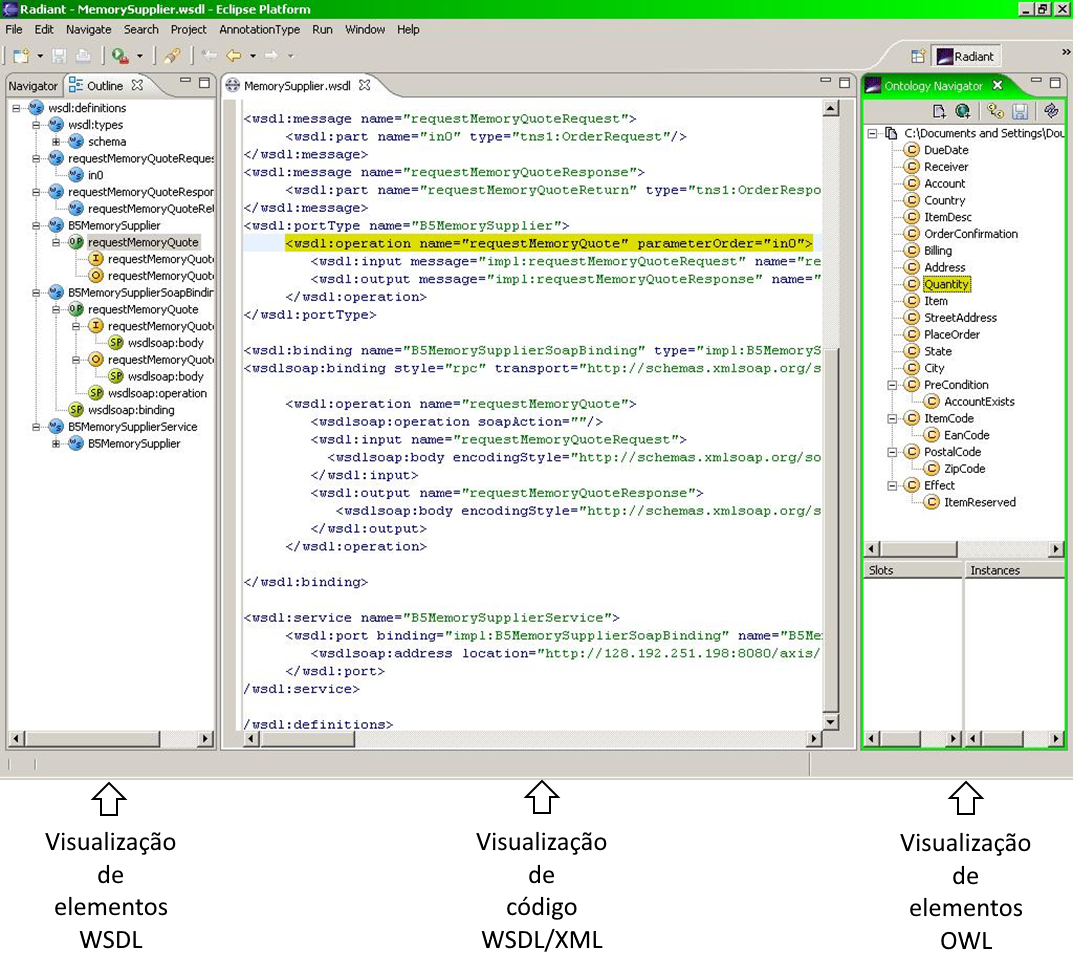
\includegraphics[scale=0.5]{2-fundamentacao-teorica/imagens/radiant3.png}
    \centering
    \caption[Interface gráfica de usuário da ferramenta Radiant.]{\textbf{Interface gráfica de usuário da ferramenta Radiant.}}
    \label{fig:radiant}
\end{figure}
\subsection{Iridescent}\label{2-fundamentacao-ferramentas-iridescent}

Iridescent~\cite{STAVROPOULOS-2013-Iridescent} é uma ferramenta \textit{standalone} que permite anotar descrições de serviços web de acordo com o padrão SAWSDL. As anotações são inseridas com base nas referências de termos de uma ontologia representada no formato OWL~\cite{W3C-2012-OWL}.

Por meio de uma interface gráfica de usuário, Iridescent permite que entidades identificadas na descrição de um serviço web sejam anotadas com os termos contidos na ontologia. A visualização de uma descrição de serviço web e uma ontologia ocorre por meio de uma representação visual no formato de árvore (\textit{tree-view}), semelhante ao \textit{plugin} Radiant~\cite{MILLER-VERMA-GOMADAM-SHETH-BREWER-2005-Radiant}.

Iridescent oferece recursos que automatizam parcialmente o processo de anotação semântica nos serviços web. A partir de um algoritmo de busca, conceitos de uma ontologia são sugeridos para os termos contidos em uma descrição de um serviço, servindo como um guia para o usuário. O usuário pode acatar ou não as sugestões da ferramenta. Iridescent também provê recursos para que os métodos \textit{Lifting Schema Mapping} e \textit{Lowering Schema Mapping} possam ser implementados e descritos no WSDL.

A utilização do recurso \textit{drag-and-drop} também auxilia o processo. O usuário pode arrastar elementos (conceitos) da representação visual de uma ontologia, do painel lateral direito, para um elemento WSDL presente no código disponibilizado pelo painel central. As anotações semânticas (SAWSDL) podem ser vistas diretamente no código WSDL/XML.

%O vínculo das anotações dos termos da ontologia com a descrição dos serviços web é realizado pela visualização do código WSDL/XML da descrição de serviço anotado semanticamente com a sintaxe SAWSDL~\cite{W3C-2007-SAWSDL}.

A \figurename~\ref{fig:iridescent} ilustra a interface gráfica de usuário de Radiant. Na lateral esquerda, encontram-se representados os elementos de uma ontologia. Na lateral direita, encontram-se representados os elementos WSDL. Finalmente, no centro, encontra-se a especificação WSDL anotada

\begin{figure}[h]
    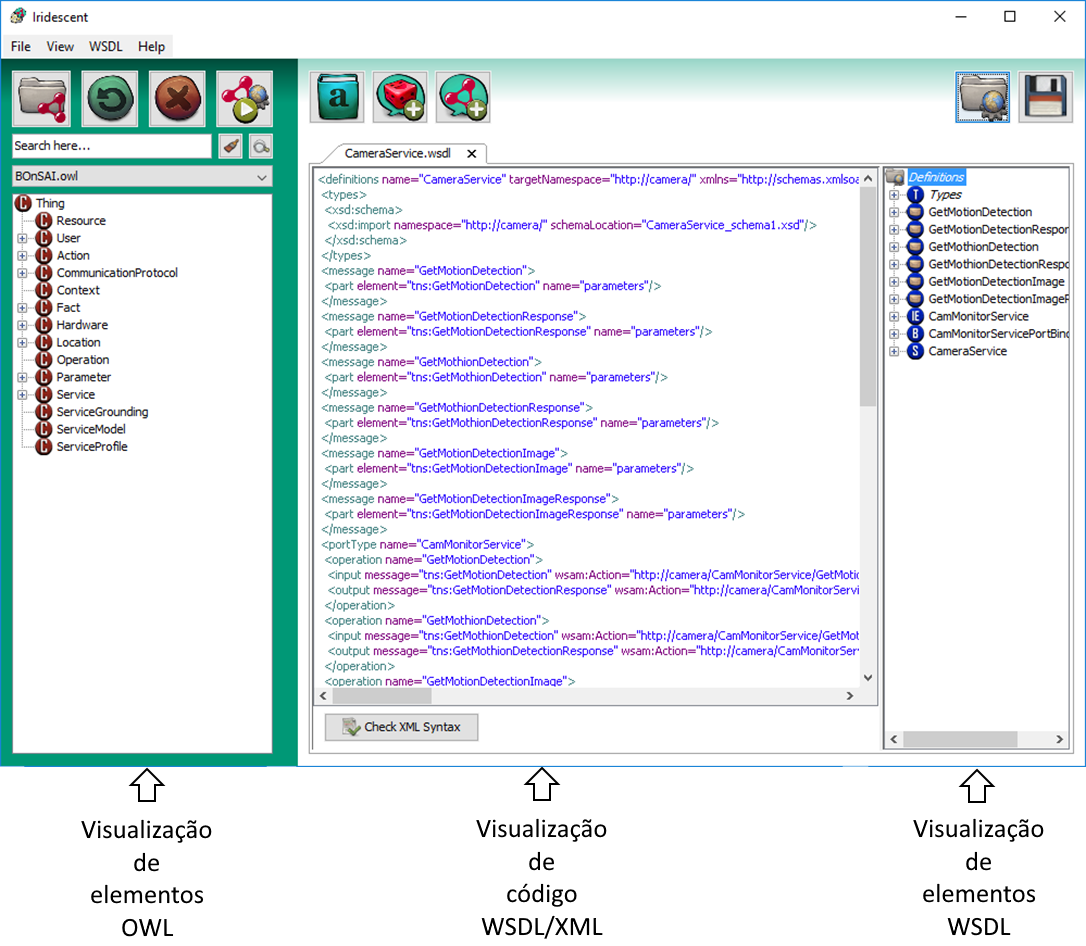
\includegraphics[scale=0.5]{2-fundamentacao-teorica/imagens/iridescent3.png}
    \centering
    \caption[Interface gráfica de usuário da ferramenta Iridescent.]{\textbf{Interface gráfica de usuário da ferramenta Iridescent.}}
    \label{fig:iridescent}
\end{figure}
\subsection{EasyWSDL \& EasySAWSDL}\label{2-fundamentacao-ferramentas-easywsdl}

EasyWSDL~\cite{EasyWSDL-2016} é uma biblioteca Java para suporte à leitura, à edição e à criação de documentos WSDL e XML Schema (XSD). EasyWSDL foi desenvolvida pelo \textit{OW2 Consortium}~\cite{OW2-2016-Site}, organização da comunidade \textit{open-source}, que tem como missão promover o desenvolvimento de aplicações \textit{middleware} e de negócio, plataformas de computação em nuvem, entre outras.

A arquitetura de EasyWSDL é extensível. Assim, a extensão EasySAWSDL~\cite{EasySAWSDL-2016} foi proposta para permitir a anotação de documentos WSDL segundo o padrão SAWSDL~\cite{W3C-2007-SAWSDL}. EasyWSDL fornece classes e métodos específicos para a criação e a manipulação de elementos de um documento WSDL, enquanto que EasySAWSDL fornece classes e métodos específicos para a anotação semântica. A manipulação de elementos WSDL e atributos SAWSDL são abstraídos por meio da linguagem de programação. A biblioteca provê métodos claros que permitem que desenvolvedores, familiarizados com a linguagem de programação Java, possam compreender e manipular mais facilmente o documento. Neste sentido, desenvolvedores não necessitam lidar diretamente com dados sintáticos das especificações WSDL e SAWSDL para a criação de serviços web semânticos.

%Por meio da arquitetura orientada a objetos da linguagem Java, EasyWSDL e sua extensão EasySAWSDL proveem um nível mais abstrato de construção e manipulação de elementos WSDL e atributos SAWSDL, dado que desenvolvedores de software normalmente estão mais familiarizados com linguagens de programação orientadas a objetos do que com os padrões WSDL e SAWSDL.

A \lstlistingname~\ref{lst:easywsdl} apresenta um exemplo de utilização da biblioteca EasySAWSDL para a anotação de uma especificação WSDL. As linhas 1 e 2 contém instruções para a leitura de um documento WSDL. O objeto \texttt{reader} é utilizado para a leitura de um documento WSDL, enquanto que o objeto \texttt{desc} é utilizado para o armazenamento de um documento WSDL. A linha 3 contém uma instrução necessária para a escrita de atributos SAWSDL. A linha 4 contém uma instrução para a leitura de uma descrição WSDL (objeto \texttt{desc}) por meio do escritor SAWSDL. A linha 5 contém uma instrução para obter um elemento WSDL (objeto \texttt{ele}) dado um identificador. Finalmente, a linha 6 contém uma instrução para adicionar um atributo \textit{Model Reference}, com o uso de uma URI de um conceito de uma ontologia.

%Refs da listagem:
% https://www.overleaf.com/learn/latex/Code_listing
% https://en.wikibooks.org/wiki/LaTeX/Source_Code_Listings
% http://texdoc.net/texmf-dist/doc/latex/listings/listings.pdf
\begin{lstlisting}[language=java,caption={[Exemplo de uso da biblioteca EasySAWSDL]\textbf{Exemplo de uso da biblioteca EasySAWSDL}.},label={lst:easywsdl}]
    WSDLReader reader = WSDLFactory.newInstance().newWSDLReader();
    Description desc = reader.read(new URL("http://grasews/svc.wsdl"));
    SAWSDLWriter writer = SAWSDLFactory.newInstance().newSAWSDLWriter();
    Document doc = writer.getDocument(desc);
    Element ele = doc.getElementById("elementId");
    ele.addModelReference(new URI("http://grasews.owl\#concept"));
\end{lstlisting}

%SAWSDLReader reader = SAWSDLFactory.newInstance().newSAWSDLReader();
\subsection{Avaliação Ferramental}\label{2-fundamentacao-ferramentas-avaliacao}

%As ferramentas Radiant, Iridescent e EasyWSDL/EasySAWSDL foram avaliadas segundo suas disponibilidades e suas usabilidades. A seguir são apresentadas características relevantes que nos auxiliaram durante esta avaliação.

%Radiant apresenta problemas quanto à sua disponibilidade. A distribuição de Radiant é realizada por meio de um plugin. A dependência do Eclipse para a sua utilização dificulta a sua adoção. O usuário deve ter um conhecimento prévio acerca da utilização do Eclipse. A configuração (instalação) do Eclipse e de Radiant no Eclipse são passos a mais que o usuário também deve realizar antes de iniciar o uso da ferramenta, o que pode contribuir para que a curva de aprendizagem de Radiant seja grande, i.e., iniciar o uso de Radiant pode requisitar um tempo adicional e não esperado. Adicionalmente, as distribuições de Radiant atualmente encontradas na Internet não são compatíveis com as versões mais recentes do Eclipse.

%Iridescent apresenta uma maior disponibilidade, visto que é uma ferramenta disponibilizada no formato \textit{standalone}. Tal formato não exige que seus usuários tenham um conhecimento prévio de outras ferramentas e tão pouco que dependam de outras distribuições. Neste sentido, a curva de aprendizagem de Iridescent é menor quando comparada com Radiant. Iridescent também apresentou erros (exceções não tratadas) durante o seu uso, o que impossibilitou sua utilização de forma fluente.

%Tanto Radiant quanto Iridescent requerem conhecimento técnico de XML/WSDL para que a anotação semântica possa ser realizada pelo usuário. Ambas ferramentas pressupõem que anotações semânticas devam ser inseridas diretamente no documento WSDL, mesmo que sejam facilitadas por meio de representações visuais dos elementos WSDL e dos elementos OWL e por recursos como \textit{drag-and-drop}.

%EasyWSDL e sua extensão EasySAWSDL foram facilmente encontradas. Por se tratar de uma biblioteca associada a uma linguagem de programação específica, esta solução possui usabilidade e aplicabilidade restritas.

%Por se tratar de uma biblioteca de desenvolvimento, EasyWSDL e EasySAWSDL também não exigem conhecimento prévio de outras ferramentas e integrações. Porém, exigem conhecimento de programação e da linguagem \textit{Java}, o que pode ser um grande desmotivador e fator bloqueante para o seu uso. Neste sentido, a biblioteca apresenta uma curva de aprendizagem maior que Radiant e Iridescent.

%A Tabela \ref{tab:formatos-distribuicao-ferramentas-disponiveis} resume os formatos de distribuição para as ferramentas apresentadas e avaliadas neste trabalho. A primeira coluna lista as ferramentas apresentadas neste trabalho. Já a segunda coluna lista os formatos de distribuição de cada ferramenta, conforme a primeira coluna.

%\begin{table}[h]
%    \setlength{\tabcolsep}{10pt} % Default value: 6pt
%    \renewcommand{\arraystretch}{2} % Default value: 1
%    \centering
%    \caption{Formatos de distribuição das ferramentas disponíveis.}
%    \label{tab:formatos-distribuicao-ferramentas-disponiveis}
%    \begin{tabular}{ | p{5cm} | p{7cm} | }
%        \hline  
%        \textbf{Ferramenta} & \textbf{Formato de Distribuição}
%        \\
%        \hline
%        {Radiant} & \textit{plugin}
%        \\
%        \hline
%        {Iridescent} & \textit{standalone}
%        \\
%        \hline
%        {EasyWSDL/EasySAWSDL} & {biblioteca de desenvolvimento (API)}
%        \\
%        \hline
%    \end{tabular}
%\end{table}

As ferramentas Radiant, Iridescent e EasyWSDL \& EasySAWSDL foram avaliadas segundo três critérios de usabilidade: i) facilidade de aprendizado, ii) maximização da produtividade e iii) minimização da taxa de erros. Facilidade de aprendizado refere-se ao esforço (tempo) necessário para aprender a utilizar a ferramenta e, portanto, atingir os resultados esperados. Quanto maior a facilidade de aprendizado, menor é a curva de aprendizagem. Maximização da produtividade refere-se à eficiência com a qual as ferramentas conseguem auxiliar seus usuários a atingirem os resultados esperados. Quanto maior a maximização da produtividade, maior é a eficiência. Finalmente, minimização da taxa de erros refere-se à facilidade com a qual exceções e fluxos não esperados executados por seus usuários. Quanto maior a minimização da taxa de erros, menor é a presença de erros.

Para realizar esta avaliação, utilizamos as três ferramentas para reproduzir parcialmente um conjunto de anotações semânticas desenvolvidas para diferentes serviços web na área de expressão gênica~\cite{GUARDIA-FARIAS-2017-SemantiSCo}. Cada diferente critério de usabilidade foi avaliado segundo uma classificação envolvendo níveis alto, médio e baixo.

No critério de facilidade de aprendizado, o \textit{plugin} Radiant foi avaliado em nível médio em razão da dificuldade associada à instalação e à configuração deste \textit{plugin}. Já a ferramenta Iridescent foi avaliada em nível alto neste critério por se tratar de uma ferramenta \textit{standalone} e, consequentemente, por não possuir dependências de outras ferramentas. Adicionalmente, Iridescent possui uma interface gráfica mais intuitiva quando comparado ao \textit{plugin} Radiant. Com isso, esta ferramenta apresentou uma maior facilidade de aprendizado em relação às demais. Finalmente, EasyWSDL \& EasySAWSDL foram avaliadas em nível baixo no critério de facilidade de aprendizado,
por se tratar de uma biblioteca de programação e, portanto, dependerem de conhecimento técnico prévio na linguagem de programação utilizada (Java).

Em relação ao critério de maximização da produtividade, as ferramentas Radiant e Iridescent foram avaliadas em nível médio, dado que, uma vez disponíveis, estas ferramentas permitiram a anotação semântica de forma simples. Entretanto, as anotações produzidas não são claramente percebidas dado que o usuário necessita visualizar a própria especificação WSDL para ter total compreensão das ações (anotações) realizadas. A biblioteca EasyWSDL \& EasySAWSDL foi avaliada em nível baixo, dada a necessidade de se criar um programa para permitir a anotação semântica de uma dada especificação WSDL.

%haja vista a sua interface gráfica não muito intuitiva 
%, devido à quantidade de passos e instruções necessárias para criar-se anotações semânticas em um documento WSDL.

Por fim, em relação ao critério de minimização da taxa de erros, Radiant e EasyWSDL \& EasySAWSDL não apresentaram erros durante sua utilização, portanto, sendo classificados em nível alto. Entretanto, Iridescent apresentou algumas falhas não tratadas ou pouco explicadas ao usuário, consequentemente, obtendo uma avaliação de nível médio.

A \tablename~\ref{tab:avaliacao-ferramentas-disponiveis} resume os critérios de usabilidade avaliados para cada ferramenta.

\begin{table}[ht!]
    \setlength{\tabcolsep}{10pt} % Default value: 6pt
    \renewcommand{\arraystretch}{1.5} % Default value: 1
    \centering
	\caption[Avaliação de usabilidade para as ferramentas disponíveis.]{\textbf{Avaliação de usabilidade para as ferramentas disponíveis.}}
	\label{tab:avaliacao-ferramentas-disponiveis}
	%\resizebox{\textwidth}{!}{
		\begin{tabular}{| >{\columncolor{Gray}}c | c | c | c | }
			\hline
            \rowcolor{Gray}
			{} & \textbf{Facilidade de} & \textbf{Maximização da} & \textbf{Minimização da}
			\\
            \rowcolor{Gray}
			\multirow{-1.5}{*}[3px]{\textbf{Ferramenta}} & \textbf{aprendizado} & \textbf{produtividade} & \textbf{taxa de erros}
			\\
			\hline
			\textbf{Radiant} & {Médio} & {Médio} & \textcolor{blue}{Alto}
			\\
            \hline
			\textbf{Iridescent} & \textcolor{blue}{Alto} & {Médio} & {Médio}
			\\ 
            \hline
			\textbf{EasySAWSDL} & \textcolor{red}{Baixo} & \textcolor{red}{Baixo} & \textcolor{blue}{Alto}
			\\
            \hline
		\end{tabular}
	%}
\end{table}
%\input{2-fundamentacao-teorica/2.5.4-owl-s-editor} % descomentar
\chapter{Notação Visual para SAWSDL}\label{3-notacao-visual-para-sawsdl}

%citar os princípios (dos 9) usados no grasews
Linguagens de modelagem são comumente utilizadas em uma organização para modelar desde regras de negócio até artefatos de \textit{software}. Diferentes princípios propostos pela Física das Notações~\cite{MOODY-2009-Physics-Notation} podem ser utilizados para criar representações visuais de um dado domínio de forma mais eficaz, contribuindo, portanto, para a criação de modelos de mais fácil compreensão.

Este capítulo apresenta uma proposta de notação visual para o desenvolvimento de serviços web semânticos utilizando o padrão SAWSDL. O capítulo está estruturado da seguinte forma: a seção \ref{3-notacao-visual-wsdl} apresenta a notação visual proposta para a representação de elementos de uma especificação WSDL; a seção \ref{3-notacao-visual-owl} apresenta a notação visual proposta para a representação de classes de ontologias OWL; a seção \ref{3-notacao-visual-sawsdl} apresenta a notação visual proposta para anotações semânticas segundo o padrão SAWSDL; e, por fim, a seção \ref{3-adequacao-aos-principios-da-fisica-das-notacoes} avalia a adequação entre as notações visuais propostas e os princípios da Física das Notações.

% o uso de notações visuais que possibilitam abstrair detalhes técnicos (sintáticos) de elementos que compõem uma descrição de serviço web segundo a especificação WSDL~\cite{W3C-2007-WSDL}, de instâncias de classes de uma ontologia OWL~\cite{W3C-2012-OWL}, bem como de anotações semânticas segundo a abordagem SAWSDL~\cite{W3C-2007-SAWSDL}
\section{Notação Visual para WSDL}\label{3-notacao-visual-wsdl}

Uma especificação WSDL pode ser representada graficamente por meio de uma estrutura de grafo. Esta estrutura facilita a compreensão dos diferentes tipos de elementos de uma especificação WSDL, bem como suas relações hierárquicas.

Os tipos de elemento de uma especificação WSDL passíveis de serem representados visualmente em uma estrutura de grafo são: \textit{wsdl:interface}, \textit{wsdl:operation}, \textit{wsdl:input}, \textit{wsdl:output}, \textit{wsdl:infault}, \textit{wsdl:outfault}, \textit{wsdl:fault}, \textit{xs:complexType} e, por fim, \textit{xs:simpleType}. Cada elemento é representado por um nó no grafo. Estes elementos são hierarquicamente dispostos no grafo em um formato de árvore, partindo do elemento mais genérico, \textit{wsdl:interface}, no topo da árvore, até o elemento mais específico, \textit{xs:simpleType}, na base da árvore.

O grafo de uma especificação WSDL é composto por cinco níveis. Os primeiros três níveis do grafo são utilizados para representar a estrutura de interfaces, de operações, de mensagens de entrada, de saída e de falhas de uma especificação WSDL, enquanto que os dois últimos níveis são utilizados para representar os tipos complexos e os tipos simples de dados XSD.

As arestas que ligam elementos (nós) do grafo são representadas por setas. Uma seta origina-se sempre em um elemento mais específico e destina-se a um elemento mais genérico. Tal representação indica a existência de uma relação entre os elementos conectados. Assim, partindo da base da árvore, elementos \textit{xs:simpleType} podem ter arestas destinadas tanto a elementos \textit{xs:complexType} quanto a elementos \textit{wsdl:input}, \textit{wsdl:output} ou \textit{wsdl:fault}. Elementos \textit{xs:complexType} podem ter arestas destinadas tanto a elementos \textit{wsdl:input}, \textit{wsdl:output} e \textit{wsdl:fault} quanto a elementos \textit{xs:complexType} mais genéricos. Elementos \textit{wsdl:fault} podem ter arestas destinadas tanto a elementos \textit{wsdl:infault}, quanto a elementos \textit{wsdl:outfault}. Elementos \textit{wsdl:input}, \textit{wsdl:output}, \textit{wsdl:infault} e \textit{wsdl:outfault} que, por sua vez, podem compôr uma operação, podem ter arestas destinadas, portanto, a elementos \textit{wsdl:operation}. Finalmente, elementos \textit{wsdl:operation} compõem uma interface, resultando em arestas destinadas a \textit{wsdl:interface}, no topo da árvore.

A \figurename~\ref{fig:grafo-wsdl-niveis} ilustra as representações visuais para cada elemento WSDL e XSD, juntamente com os níveis da estrutura hierárquica do formato de árvore. Na lateral esquerda, podemos visualizar as representações visuais dos elementos do grafo juntamente com suas cardinalidades. No centro, podemos visualizar os tipos de elementos WSDL e XSD relacionados às suas representações visuais. Por fim, na lateral direita, podemos visualizar os níveis que definem a estrutura hierárquica do grafo.

\begin{figure}[h]
    %\resizebox{\textwidth}{!}{
    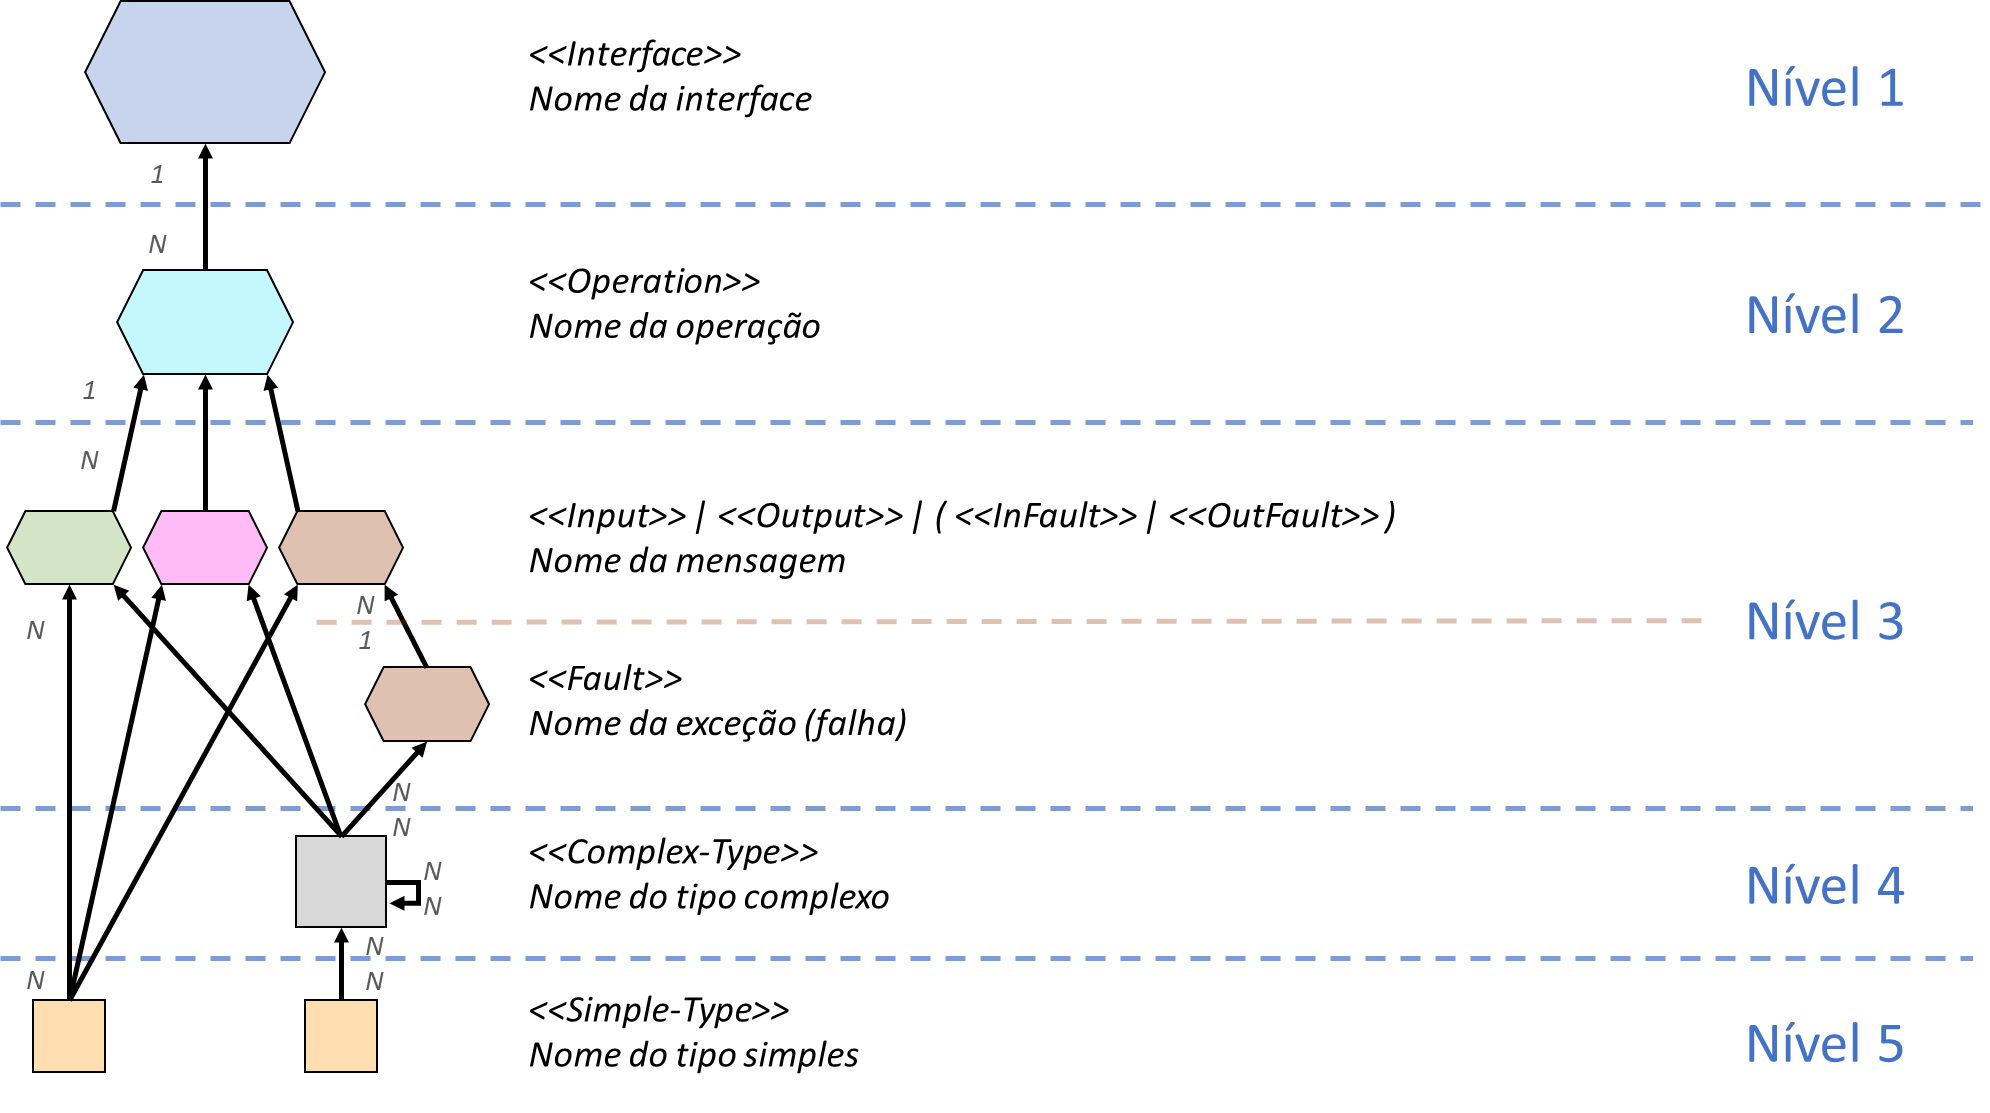
\includegraphics[scale=0.3]{3-notacao-visual-sawsdl/imagens/grafo-wsdl-niveis.PNG}
    %}
    \centering
    \caption[Representações visuais de elementos WSDL]{\textbf{Representações visuais de elementos WSDL.}}
    \label{fig:grafo-wsdl-niveis}
\end{figure}

O quinto nível do grafo (nível 5) consiste da representação visual de elementos XSD do tipo \textit{xs:simpleType}. Estes elementos podem ser utilizados tanto para compor elementos \textit{xs:complexType} quanto para compor elementos \textit{wsdl:input}, \textit{wsdl:output} e/ou \textit{wsdl:fault}. A representação visual de elementos \textit{xs:simpleType} possui o formato geométrico de um quadrado na cor laranja. Dado que estes elementos consistem do último nível do grafo, pode haver arestas partindo destes elementos e destinadas tanto a elementos \textit{xs:complexType} (nível 4) quanto a elementos \textit{wsdl:input}, \textit{wsdl:output} e/ou \textit{wsdl:fault} (nível 3). A cardinalidade dos elementos do quinto nível em relação aos elementos do quarto nível é de N para M (N:M), onde N (nível 5) pode variar entre zero ou várias instâncias (0..*) e M (nível 4) pode variar entre uma ou várias instâncias (1..*). A cardinalidade dos elementos do quinto nível em relação aos elementos do terceiro nível é de N para M (N:M), onde N (nível 5) pode variar entre zero ou várias instâncias (0..*) e M (nível 3) pode variar entre uma ou várias instâncias (1..*). Com isso, pode haver múltiplos elementos no quinto nível relacionados a múltiplos elementos do quarto nível e no terceiro nível. Entretanto, o nível 5 pode ser opcional, pois elementos \textit{xs:complexType} não necessariamente precisam ser estruturados em termos de elementos \textit{xs:simpleType}.

O quarto nível do grafo (nível 4) consiste da representação visual de elementos XSD do tipo \textit{xs:complexType}. Esta representação visual também possui o formato geométrico de um quadrado. Porém, \textit{xs:complexType} possui um tamanho maior em relação aos elementos \textit{xs:simpleType} do nível anterior (nível 5). Adicionalmente, a cor cinza é utilizada para sua representação. Dado que estes elementos consistem do quarto nível do grafo, pode haver arestas partindo destes elementos e destinadas a elementos \textit{wsdl:input}, \textit{wsdl:output} e/ou \textit{wsdl:fault}, no nível 3. Adicionalmente, dado que um elemento \textit{xs:complexType} pode ser composto tanto por outros elementos \textit{xs:complexType} quanto por elementos \textit{xs:simpleType}, podemos ter um número variável de composições, resultando em tantos sub-níveis quantos forem necessários a fim de representar tais composições. Com isso, o nível 4 do grafo poder possuir múltiplos sub-níveis. A cardinalidade dos elementos do quarto nível em relação aos elementos do terceiro nível é de N para M (N:M), onde N (nível 4) pode variar entre uma ou várias instâncias (1..*) e M (nível 3) pode variar entre uma ou várias instâncias (1..*). Assim, pode haver múltiplos elementos no quarto nível relacionados a múltiplos elementos do terceiro nível. Entretando, o nível 4 pode ser opcional desde que o nível 5 esteja presente, pois \textit{wsdl:input}, \textit{wsdl:output} e \textit{wsdl:fault} podem ser exclusivamente compostos por elementos \textit{xs:simpleType}.

O terceiro nível do grafo (nível 3) consiste da representação visual das mensagens de entrada e saída, juntamente com as mensagens de falhas e as definições de exceções tratadas por estas falhas. Com isso, no nível 3, podemos representar os elementos WSDL dos tipos \textit{wsdl:input}, \textit{wsdl:output}, \textit{wsdl:infault}, \textit{wsdl:outfault} e, finalmente, \textit{wsdl:fault}. Estas representações visuais possuem o formato geométrico de um hexágono irregular. Porém, estes elementos se diferem pela cor: a representação de \textit{wsdl:input} possui a cor verde; a representação de \textit{wsdl:output} possui a cor rosa; por fim, a representação dos elementos \textit{wsdl:infault}, \textit{wsdl:outfault} e \textit{wsdl:fault} possui a cor marrom. Os cinco elementos possuem o mesmo tamanho.

Para os elementos \textit{wsdl:input}, \textit{wsdl:output}, \textit{wsdl:infault} e \textit{wsdl:outfault}, há arestas partindo destes elementos e destinadas a elementos \textit{wsdl:operation}, no próximo nível (nível 2). Estas arestas indicam que \textit{wsdl:input}, \textit{wsdl:output}, \textit{wsdl:infault} e \textit{wsdl:outfault} compõem um elemento \textit{wsdl:operation}. Para elementos \textit{wsdl:fault}, pode haver arestas destinadas tanto a elementos \textit{wsdl:infault} quanto a \textit{wsdl:outfault}. Estas arestas indicam que \textit{wsdl:fault} pode compor tanto \textit{wsdl:infault} quanto \textit{wsdl:outfault}. A cardinalidade de elementos \textit{wsdl:input}, \textit{wsdl:output}, \textit{wsdl:infault} e \textit{wsdl:outfault}, do terceiro nível, em relação a elementos \textit{wsdl:operation}, do segundo nível, é de N para 1 (N:1), onde N (nível 3) pode variar entre zero ou várias instâncias (0..*). A cardinalidade de elementos \textit{wsdl:fault} em relação a elementos \textit{wsdl:infault} e \textit{wsdl:outfault}, todos no mesmo nível (nível 3), é de 1 para N (1:N). O nível 3 está sempre presente na estrutura hierárquica de uma especificação WSDL.

O segundo nível do grafo (nível 2) consiste da representação visual de elementos WSDL do tipo \textit{wsdl:operation}. Estas representações visuais também possuem o formato geométrico de um hexágono irregular. Porém, estes elementos são representados na cor ciano e em um tamanho maior em comparação aos elementos do nível anterior (nível 3). Dado que estes elementos consistem do segundo nível do grafo, há arestas originadas nestes elementos e destinadas a um elemento \textit{wsdl:interface}, do próximo nível (nível 1). Estas arestas indicam que elementos \textit{operation} compõem uma \textit{wsdl:interface}. A cardinalidade dos elementos do segundo nível em relação aos elementos do primeiro nível é de N para 1 (N:1), onde N (nível 2) pode variar entre uma ou mais instâncias (1..*). Com isso, pode haver múltiplos elementos no segundo nível, mas eles só podem estar relacionados a um único elemento do primeiro nível. O nível 2 está sempre presente na estrutura hierárquica de uma especificação WSDL.

Por fim, o primeiro nível do grafo (nível 1), topo da árvore, consiste da representação visual de elementos WSDL to tipo \textit{wsdl:interface}. Estas representações visuais possuem o formato geométrico de um hexágono irregular na cor azul. Dado que estes elementos consistem do primeiro nível da árvore, não há arestas originadas deles. O nível 1 também está sempre presente na estrutura hierárquica do grafo WSDL.

Além das diferentes cores, tamanhos e formas, os elementos do grafo são também identificados por textos (estereótipos) posicionados no canto superior esquerdo em relação ao nó do grafo. Para os elementos \textit{wsdl:interface}, o estereótipo \texttt{<<Interface>>} é utilizado. Para os elementos \textit{wsdl:operation}, o estereótipo \texttt{<<Operation>>} é utilizado. Para os elementos \textit{wsdl:input}, o estereótipo \texttt{<<Input>>} é utilizado. Para os elementos \textit{wsdl:output}, o estereótipo \texttt{<<Output>>} é utilizado. Para os elementos \textit{wsdl:infault}, o estereótipo \texttt{<<InFault>>} é utilizado. Para os elementos \textit{wsdl:outfault}, o estereótipo \texttt{<<OutFault>>} é utilizado. Para os elementos \textit{wsdl:fault}, o estereótipo \texttt{<<Fault>>} é utilizado. Para os elementos \textit{xs:complexType}, o estereótipo \texttt{<<Complex-Type>>} é utilizado. Por fim, para os elementos \textit{xs:simpleType}, o estereótipo \texttt{<<Simple-Type>>} é utilizado.

A \figurename~\ref{fig:grafo-wsdl} ilustra o uso da notação proposta para a representação de diferentes elementos da especificação WSDL. Uma inferface \texttt{BookStoreService} é composta pela operação \texttt{GetBook}. Esta operação, por sua vez, é composta pelas mensagens \texttt{GetBookRequest} (entrada), \texttt{GetBookResponse} (saída) e \texttt{BookNotFoundException} (falha de saída). A mensagem de entrada, \texttt{GetBookRequest}, utiliza o tipo de dado complexo \texttt{Book}, que por sua vez é composto pelo tipos simples \texttt{BookName} e \texttt{BookId}. A mensagem de saída, \texttt{GetBookResponse}, utiliza o tipo de dado complexo \texttt{ArrayOfBooks}.  \texttt{ArrayOfBooks} por sua vez utiliza o tipo complexo \texttt{Book}, o qual é composto pelos  tipos simples \texttt{BookName} e \texttt{BookId}. Por fim, a mensagem de falha de saída \texttt{BookNotFoundException} é composta pela falha \texttt{BookNotFoundException}. Esta falha utiliza o tipo complexo \texttt{BookNotFound}, o qual é composto pelo tipo simples \texttt{BookId}.

\begin{figure}[h]
    %\resizebox{\textwidth}{!}{
    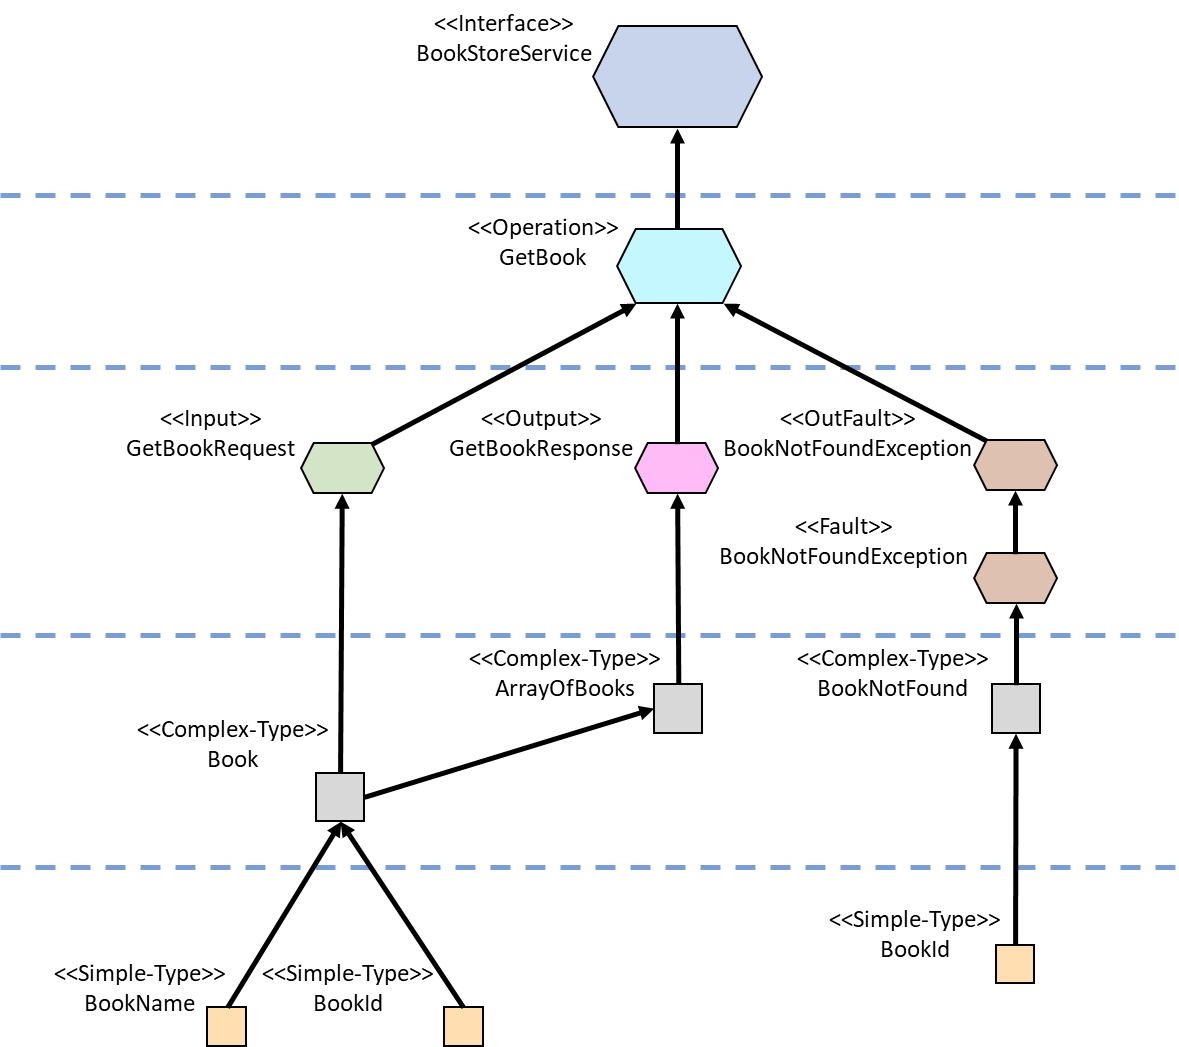
\includegraphics[scale=0.4]{3-notacao-visual-sawsdl/imagens/grafo-wsdl.PNG}
    %}
    \centering
    \caption[Representações visuais de elementos WSDL juntamente com a codificação dupla]{\textbf{Representações visuais de elementos WSDL juntamente com seus estereótipos.}}
    \label{fig:grafo-wsdl}
\end{figure}
\section{Notação Visual para OWL}\label{3-notacao-visual-owl}

As classes que compõem uma ontologia OWL também podem ser representadas graficamente por meio de uma estrutura de grafo. Esta estrutura facilita a compreensão de diferentes classes de uma ontologia, bem como suas relações hierárquicas.

Uma classe OWL é representada por meio de um círculo na cor vermelha no contexto deste trabalho. Dado o intuito de representar visualmente anotações semânticas segundo o padrão SAWSDL, nem todas as classes de uma ontologia OWL precisam ser graficamente representadas em um grafo, apenas as classes diretamente utilizadas em uma anotação (atributo do tipo \textit{sawsdl:modelReference}).

Uma classe OWL pode especializar uma classe base. A especialização entre classes pode ser visualmente representada por meio de uma seta. Uma seta origina-se sempre de uma classe mais específica e destina-se a uma classe mais genérica (classe base). Os elementos do grafo da ontologia são também identificados por textos (estereótipos) posicionados no canto superior esquerdo em relação ao nó do grafo. Estes estereótipos contém o nome da ontologia da qual o conceito (classe OWL) em uso faz parte. A \figurename~\ref{fig:grafo-owl} ilustra um grafo OWL representando três classes. A classe \texttt{Classe\_C} é uma especialização da classe \texttt{Classe\_B}, que por sua vez é uma especialização da classe \texttt{Classe\_A}. Todas estas classes fazem parte de uma mesma ontologia \texttt{Ontologia\_X}.

\begin{figure}[h]
    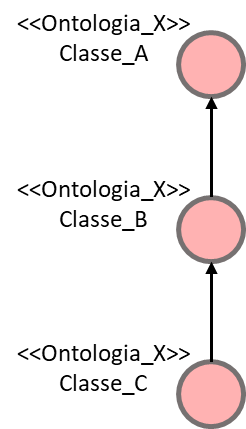
\includegraphics[scale=0.5]{3-notacao-visual-sawsdl/imagens/grafo-owl.png}
    \centering
    \caption[Representação visual em formato de grafo para classes OWL]{\textbf{Representação visual em formato de grafo para classes OWL.}}
    \label{fig:grafo-owl}
\end{figure}

Por fim, caso haja classes hierarquicamente dispostas entre duas outras classes OWL que são utilizadas em anotações semânticas e, consequentemente, já representadas visualmente no grafo, estas classes intermediárias são também visualmente representadas. Por exemplo, na \figurename~\ref{fig:grafo-owl}, caso as classes utilizadas em anotações semânticas sejam apenas as classes \texttt{Classe\_A} e \texttt{Classe\_C}, a classe \texttt{Classe\_B} será automaticamente representada visualmente, visto que ela encontra-se disposta hierarquicamente entre as duas outras classes. A representação visual de classes intermediárias independe da quantidade das mesmas.

%sejam representadas no grafo, por estarem sendo utilizadas em anotações semânticas, e estas duas classes possuírem alguma relação hierárquica, mesmo que seja por meio de outras classes intermediando esta relação, estas classes intermediárias são também visualmente representadas no grafo.

\section{Notação Visual para Atributos SAWSDL}\label{3-notacao-visual-sawsdl}

Uma especificação SAWSDL é essencialmente obtida por meio da junção dos grafos WSDL e OWL. Elementos WSDL/XSD anotados, independentemente do tipo de atributo SAWSDL (\textit{Model Reference} ou \textit{Schema Mapping}), possuem um brilho mais forte em relação aos elementos não anotados. Entretanto, quando anotados com o atributo \textit{Model Reference}, os elementos possuem uma borda grossa e vermelha. Tal característica facilita a identificação de elementos já anotados com \textit{Model Reference} em comparação a elementos não anotados. Adicionalmente, os elementos anotados com \textit{Model Reference} possuem uma aresta (linha tracejada na cor vermelha) ligando-os a uma ou mais classes OWL. A \figurename~\ref{fig:grafo-wsdl-nao-anotado-e-anotado}a ilustra elementos WSDL/XSD não anotados com \textit{Model Reference}, enquanto que a \figurename~\ref{fig:grafo-wsdl-nao-anotado-e-anotado}b ilustra elementos WSDL/XSD anotados.

\begin{figure}[h]
    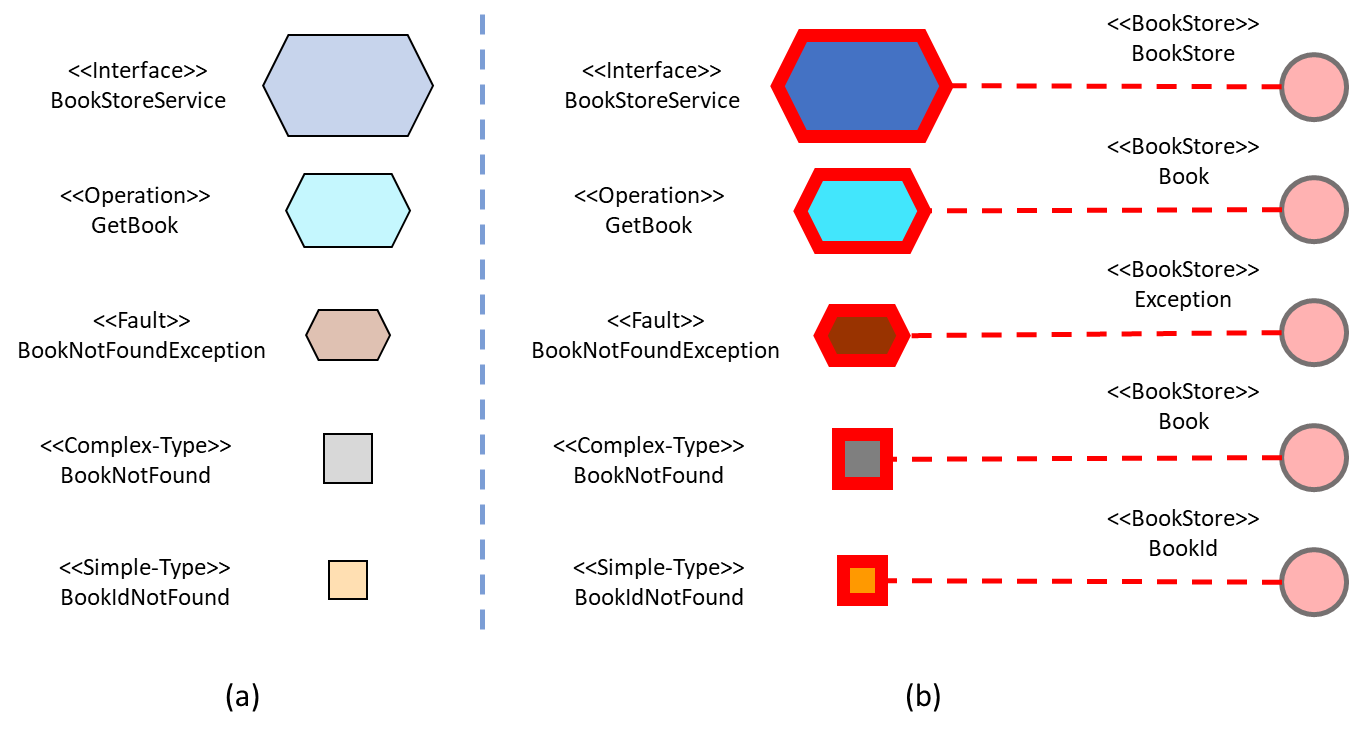
\includegraphics[scale=0.4]{3-notacao-visual-sawsdl/imagens/grafo-wsdl-nao-anotado-e-anotado.png}
    \centering
    \caption[Notação visual para elementos WSDL/XSD anotados com \textit{Model Reference}]{\textbf{Notação visual para elementos WSDL/XSD anotados com \textit{Model Reference}.} (a) Elementos WSDL/XSD não anotados. (b) Elementos WSDL/XSD anotados com classes OWL.}
    \label{fig:grafo-wsdl-nao-anotado-e-anotado}
\end{figure}

%No topo, um elemento do tipo \textit{<wsdl:interface>} é exemplificado e anotado semanticamente por meio do atributo \textit{<sawsdl:modelReference>} utilizando uma classe OWL. Abaixo de \textit{<wsdl:interface>}, um elemento do tipo \textit{<wsdl:operation>} é exemplificado e anotado semanticamente por meio do atributo \textit{<sawsdl:modelReference>} utilizando uma classe OWL. Abaixo de \textit{<wsdl:operation>}, um elemento do tipo \textit{<wsdl:input>} é exemplificado e anotado semanticamente por meio do atributo \textit{<sawsdl:modelReference>} utilizando uma classe OWL. Abaixo de \textit{<wsdl:input>}, um elemento do tipo \textit{<wsdl:output>} é exemplificado e anotado semanticamente por meio do atributo \textit{<sawsdl:modelReference>} utilizando uma classe OWL. Abaixo de \textit{<wsdl:output>}, um elemento do tipo \textit{<wsdl:fault>} é exemplificado e anotado semanticamente por meio do atributo \textit{<sawsdl:modelReference>} utilizando uma classe OWL. Abaixo de \textit{<wsdl:fault>}, um elemento do tipo \textit{<xs:complexType>} é exemplificado e anotado semanticamente por meio do atributo \textit{<sawsdl:modelReference>} utilizando uma classe OWL. Por fim, abaixo de \textit{<xs:complexType>}, um elemento do tipo \textit{<xs:simpleType>} é exemplificado e anotado semanticamente por meio do atributo \textit{<sawsdl:modelReference>} utilizando uma classe OWL.

Quando os elementos WSDL/XSD são anotados com o atributo \textit{Schema Mapping}, estes elementos possuem uma borda dupla. Tal característica facilita a identificação de elementos já anotados com \textit{Schema Mapping} em comparação a elementos não anotados.

A \figurename~\ref{fig:grafo-wsdl-anotado-model-reference-e-schema-mapping} ilustra um grafo WSDL com diferentes anotações SAWSDL. O tipo complexo \texttt{Book} e a operação \texttt{GetBook} ilustram elementos WSDL anotados apenas com o atributo \textit{Model Reference}. O tipo complexo \texttt{BookNotFound} e o tipo simples \texttt{BookId} ilustram elementos WSDL anotados apenas com um atributo \textit{Schema Mapping}. Finalmente, o tipo simples \texttt{BookName} ilustra um elemento WSDL anotado tanto com o atributo \textit{Model Reference} quanto com um atributo \textit{Schema Mapping}. Este elemento possui uma borda dupla na cor vermelha.

\begin{figure}[h]
    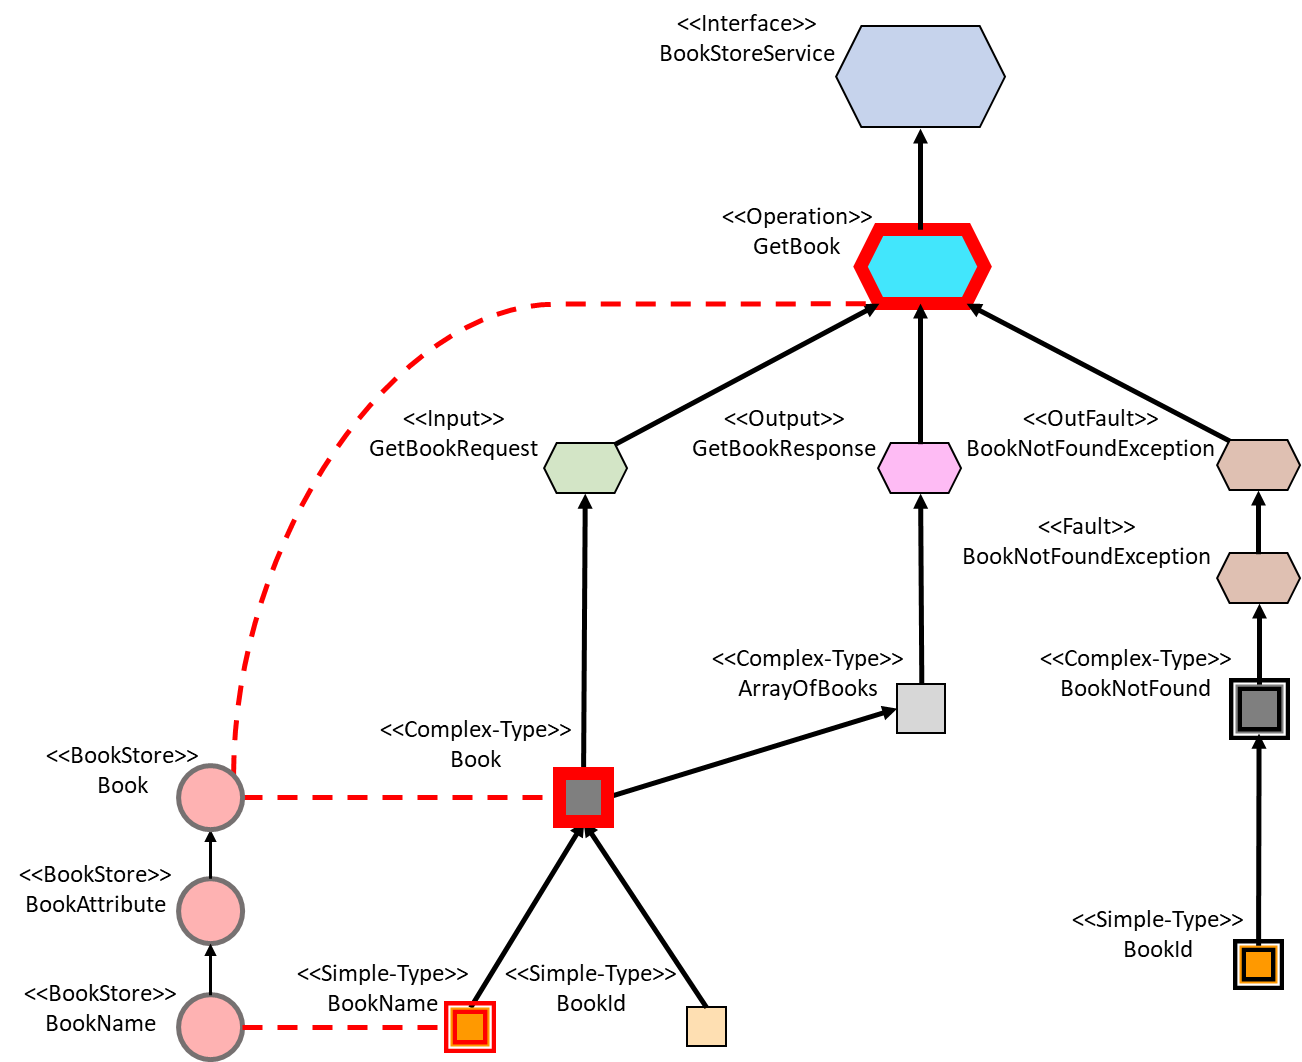
\includegraphics[scale=0.4]{3-notacao-visual-sawsdl/imagens/grafo-wsdl-anotado-model-reference-e-schema-mapping.png}
    \centering
    \caption[Exemplo de grafo WSDL com anotações utilizando tanto \textit{Model Reference} quanto \textit{Schema Mapping}]{\textbf{Exemplo de grafo WSDL com anotações utilizando tanto \textit{Model Reference} quanto \textit{Schema Mapping}.}}
    \label{fig:grafo-wsdl-anotado-model-reference-e-schema-mapping}
\end{figure}
\section{Adequação aos princípios da Física das Notações}\label{3-adequacao-aos-principios-da-fisica-das-notacoes}

Dentre os nove princípios da Física das Notações, os princípios Clareza Semiótica, Diferenciação Perceptiva, Expressividade Visual, Codificação Dupla e Economia Gráfica foram aplicados ao desenvolvimento da notação visual para SAWSDL. Os demais princípios não possuem aplicação para o propósito deste trabalho.

%\textbf{Princípio da Clareza Semiótica}

O princípio da Clareza Semiótica foi aplicado de modo que elementos de uma especificação WSDL e classes de uma ontologia possuam uma representação visual clara. Todos os elementos de uma especificação WSDL são visualmente representados com o propósito de facilitar o processo de anotação semântica. Os elementos \textit{wsdl:input}, \textit{wsdl:output}, \textit{wsdl:infault} e \textit{wsdl:outfault}, apesar de não serem passíveis de anotação semântica, são visualmente representados de modo a facilitar a compreensão da especificação WSDL. Em relação às classes OWL, classes que não são utilizadas em uma anotação semântica ou que não sejam hierarquicamente dispostas entre classes que são utilizadas em uma anotação semântica não são visualmente representadas.

%\textbf{Princípio da Diferenciação Perceptiva}

O princípio da Diferenciação Perceptiva foi aplicado de modo a tornar as notações visuais propostas por este trabalho claramente distinguíveis umas das outras. Esta distinção ocorre por meio do uso (combinado) dos princípios da Expressividade Visual e da Codificação Dupla, ambos explicados a seguir. Desta forma, entende-se que os diferentes elementos visuais representados no grafo são facilmente identificados pelo usuário.

%\textbf{Princípio da Expressividade Visual}

O princípio da Expressividade Visual foi satisfeito visto que das sete variáveis propostas por este princípio, seis foram utilizadas neste trabalho. A variável posição é aplicada entre os diferentes tipos de elementos WSDL e XSD, de modo a representar quais elementos são compostos por outros elementos da especificação WSDL. A variável tamanho é aplicada entre os diferentes tipos de elementos WSDL conforme seus níveis. A variável brilho foi utilizada a fim de diferenciar elementos WSDL/XSD anotados semanticamente dos elementos não anotados. A variável cor foi utilizada na representação de todos elementos do grafo, a fim de facilitar a diferenciação entre diferentes tipos de elementos da especificação WSDL, de elementos de classes OWL e, por fim, de anotações semânticas (arestas entre elementos WSDL/XSD e classes OWL). A variável orientação foi utilizada nos sentidos das arestas (setas). Entre elementos WSDL/XSD, a orientação da seta diferencia elementos que são compostos por outros elementos. Já entre elementos OWL, a orientação da seta diferencia elementos que especializam outros elementos. Finalmente, o uso da variável forma contribui para a diferenciação entre elementos WSDL (interfaces, operações e mensagens) e elementos XSD (tipos complexos e simples) de uma especificação WSDL e elementos OWL (classes de uma ontologia OWL). Apenas a variável textura não foi utilizada no contexto deste trabalho.

%\textbf{Princípio da Codificação Dupla}

O princípio da Codificação Dupla foi aplicado por meio do uso de diferentes estereótipos juntamente com as representações visuais. Desta forma, a compreensão dos diferentes tipos de elementos visualmente representados no grafo é facilitada.

%\textbf{Princípio da Economia Gráfica}

Finalmente, o princípio da Economia Gráfica foi satisfeito, pois utilizamos uma quantidade mínima de elementos visuais de modo a facilitar a compreensão de uma especificação WSDL e de elementos envolvidos na anotação semântica segundo o padrão SAWSDL. Os tipos elementos que possuem representações visuais variam entre: \textit{wsdl:interface}, \textit{wsdl:operation}, \textit{wsdl:input}, \textit{wsdl:output}, \textit{wsdl:infault}, \textit{wsdl:outfault}, \textit{wsdl:fault}, \textit{xs:complexType} e \textit{xs:simpleType} para elementos WSDL/XSD; e classes para elementos de uma ontologia OWL.

%Os princípios do Ajuste Cognitivo (seção \ref{2-fundamentacao-notacao-visual-principio-ajuste-cognitivo}), da Complexidade Gerenciável (seção \ref{2-fundamentacao-notacao-visual-principio-complexidade-gerenciavel}) e da Transparência Semântica (seção \ref{2-fundamentacao-notacao-visual-principio-transparencia-semantica}) não foram satisfeitos totalmente. O princípio do Ajuste Cognitivo não foi necessário satisfazer pois o público alvo é bem exclusivo: ou desenvolvedores de serviços ou especialistas de domínio. O princípio da Complexidade Gerenciável não foi necessário satisfazer pois o diagrama já possui uma grande Economia Gráfica e a pequena quantidade elementos passíveis de serem representados para a anotação semântica já limitou, consequentemente, a quantidade de recursos visuais necessários na representação visual. Portanto, não houve necessidade de aplicarmos a modularização nem a hierarquização do modelo. Por fim, o princípio Transparência Semântica não foi possível ser satisfeito dada a limitação de customização dos elementos visuais disponíveis biblioteca de desenvolvimento utilizada neste trabalho. Neste sentido, não chegamos a um consenso de customizações visuais necessárias a fim de atender a este princípio e que, ao mesmo tempo, possuíssem uma interface gráfica com boa usabilidade. % descomentar
\chapter{Ferramenta Grasews}\label{4-grasews}

Este capítulo apresenta a ferramenta \textit{Graphical Annotation of Semantic Web Services} (Grasews) de suporte gráfico e colaborativo à anotação semântica de serviços web desenvolvida neste trabalho. O capítulo apresenta uma visão geral de sua arquitetura, principais tecnologias utilizadas em sua implementação e principais aspectos associados ao suporte à anotação semântica colaborativa de serviços web.

Este capítulo está estruturado da seguinte forma: a seção \ref{4-grasews-arquitetura} apresenta a arquitetura de desenvolvimento da ferramenta Grasews; a seção \ref{4-grasews-visao-geral-implementacao} apresenta uma visão geral da implementação da ferramenta Grasews; a seção \ref{4-grasews-suporte-anotacao} apresenta o suporte à anotação semântica por meio do grafo de Grasews; a seção \ref{4-grasews-menu-tree-view} apresenta o suporte à anotação semântica por meio dos menus \textit{tree-view} de uma especificação WSDL e de uma ontologia OWL da ferramenta Grasews; e, por fim, a seção \ref{4-grasews-suporte-edicao-colaborativa} apresenta o suporte à anotação semântica de forma colaborativa provido pela ferramenta Grasews.
\section{Arquitetura de Grasews}\label{4-grasews-arquitetura}

%A ferramenta consiste de um sistema web que consome um conjunto de serviços disponibilizados por uma API (\textit{Application Programming Interface}). Utilizamos o \textit{Postgres}~\cite{POSTGRES-2019} como o sistema gerenciador de banco de dados (SGBD).
%Ambos foram hospedados na plataforma \textit{online} \textit{Microsoft Azure} (\textit{Cloud Computing Platform \& Services})~\cite{MICROSOFT-2019-AZURE}

Esta seção apresenta uma visão geral acerca da arquitetura de desenvolvimento de Grasews, juntamente com uma visão detalhada dos módulos da arquitetura e as integrações destes módulos.

\subsection{Visão Geral}\label{4-grasews-arquitetura-visao-geral}

O desenvolvimento de Grasews segue a abordagem de desenvolvimento \textit{Domain-Driven Design} (DDD)~\cite{EVANS-2004-DDD}. 
A \figurename~\ref{fig:grasews-architectural-projects} apresenta os módulos existentes na arquitetura de Grasews distribuídos nas camadas da abordagem DDD.

\begin{figure}[h]
    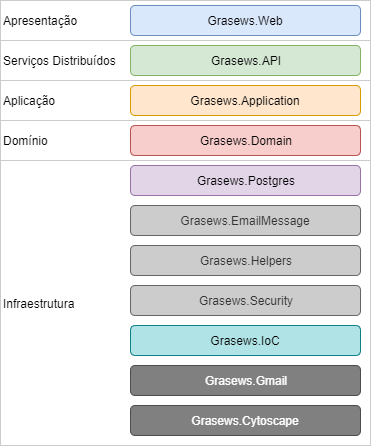
\includegraphics[scale=0.7]{4-grasews/imagens/grasews-architectural-projects.png}
    \centering
    \caption[Camadas e módulos da arquitetura da ferramenta Grasews]{\textbf{Camadas e módulos da arquitetura da ferramenta Grasews.}}
    \label{fig:grasews-architectural-projects}
\end{figure}

\newpage

A partir da abordagem DDD, a solução implementada consiste de cinco (5) camadas:

\begin{enumerate}

  \item
  \textit{\textbf{Apresentação}}:
  
  Esta camada de \textit{front-end} é composta pelo módulo \texttt{Grasews.Web}, que provê a interface gráfica de usuário (UI) da ferramenta.
  
  \item
  \textit{\textbf{Serviços Distribuídos}}:
  
  Esta camada é composta pelo módulo \texttt{Grasews.API}, que provê uma API para expor as funcionalidades do \textit{back-end} de Grasews. Esta API consiste de um conjunto de operações disponibilizadas por meio de serviços web RESTful. Todas as ações executadas por um usuário que necessitam interação com os demais módulos do lado servidor (\textit{back-end}) da aplicação são exclusivamente realizadas através da API.
  
  \item
  \textit{\textbf{Aplicação}}:
  
  Esta camada de \textit{back-end} é composta pelo módulo \texttt{Grasews.Application}, responsável por orquestrar as regras de negócio da aplicação.
  
  \item
  \textit{\textbf{Domínio}}:
  
  Esta camada de \textit{back-end} é composta pelo módulo \texttt{Grasews.Domain}, responsável por definir as regras de negócio da aplicação e as entidades de domínio do negócio. As regras de negócio são providas por meio de interfaces de desenvolvimento contidas neste módulo. Os demais módulos da aplicação seguem regras ditadas pelo módulo \texttt{Grasews.Domain}. A arquitetura de Grasews possui o seu desenvolvimento orientado a interfaces e não a implementações de classes. Tal característica facilita a substituição de um módulo da aplicação por outro módulo que, por exemplo, utiliza outra tecnologia diferente. Por exemplo, caso optemos por não usar mais o SGBD \textit{Postgres}, substituindo-o pelo SGBD \textit{Microsoft SQL Server}\cite{SQLSERVER-2019}, basta substituirmos o módulo \texttt{Grasews.Postgres} por, por exemplo, o módulo \texttt{Grasews.SqlServer}, o qual utilizaria as bibliotecas apropriadas para o acesso ao novo banco de dados. Adicionalmente, por meio das interfaces de  \texttt{Grasews.Domain}, garantimos que toda a aplicação funcione seguindo regras definidas pelo domínio (núcleo da aplicação).
  
  \item
  \textit{\textbf{Infraestrutura}}:
  
  Esta camada de \textit{back-end} é subdivida em três subcamadas de módulos: i) acesso a dados; ii) corte transversal; e iii) serviços externos.  A subcamada de acesso a dados é composta pelo módulo \texttt{Grasews.Postgres}, responsável por conectar a aplicação ao SGBD Postgres~\cite{POSTGRES-2019}. A subcamada de corte transversal é composta pelos módulos \texttt{Grasews.EmailMessage}, \texttt{Grasews.Helpers}, \texttt{Grasews.Security} e \texttt{Grasews.IoC}. O módulo \texttt{Grasews.EmailMessage} provê suporte à construção de mensagens de \textit{e-mail}. O módulo \texttt{Grasews.Helpers} provê suporte funcional às demais camadas e, consequentemente, aos demais módulos. Por exemplo, funcionalidades de suporte à leitura de XML, funcionalidades de suporte à manipulação de enumeradores e funcionalidades de suporte à requisições HTTP entre o \textit{front-end} e a API. O módulo \texttt{Grasews.Security} provê suporte à funcionalidades de segurança da aplicação. Por exemplo, funcionalidades de suporte à autenticação e permissões de um usuário. Finalmente, o módulo \texttt{Grasews.IoC} provê suporte funcional à inversão de controle (\textit{inversion of control} - IoC) e à injeção de dependências (\textit{dependency injection} - DI).
  
  A inversão de controle é uma técnica utilizada para reduzir o acoplamento entre objetos (classes) de uma arquitetura de \textit{software}. A arquitetura de um projeto pode ser severamente prejudicada quando tem-se um alto acoplamento, podendo tornar a sua manutenção custosa e até mesmo dificultar a sua evolução.
  
  A injeção de dependências é uma forma de se aplicar a inversão de controle, garantindo então um baixo acoplamento em um conjunto de classes. O padrão de injeção de dependência é baseado em abstrações das classes, por meio de classes abstratas ou interfaces de desenvolvimento. Segundo este padrão, o desenvolvimento é orientado à interface de uma classe ao invés de sua verdadeira implementação. A injeção de dependências de Grasews é feita por meio da injeção de objetos (dependências) por meio de construtores. Com isso, uma classe que necessita de instâncias de outras classes (dependências) obtém tais instâncias por meio da injeção destes objetos no construtor desta classe dependente.
  
  Por fim, a camada de serviços externos é composta pelos módulos \texttt{Grasews.Cytoscape} e \texttt{Grasews.Gmail}. O módulo de serviço externo \texttt{Grasews.Cytoscape} provê suporte à construção dos grafos WSDL e OWL da ferramenta. Este módulo utiliza a biblioteca \textit{Cytoscape.js}~\cite{CYTOSCAPE-2015}. Já o módulo de serviço externo \texttt{Grasews.Gmail} provê suporte ao envio de mensagens de \textit{e-mail} aos usuários por meio do serviço do \textit{Gmail}~\cite{GOOGLE-2019-GMAIL}.
  
\end{enumerate}
\subsection{Interações entre Módulos Grasews}\label{4-grasews-interacoes-modulos}

A \figurename~\ref{fig:grasews-architecture-simplified} apresenta uma visão geral das principais interações existentes entre os módulos Grasews. Uma seta preta e sólida representa as interações de um usuário com a aplicação. Uma linha azul, sólida e com setas sólidas nas duas extremidades representa interações entre os módulos utilizando objetos, i.e., instâncias de classes conforme a programação orientada a objetos. Uma linha rosa e tracejada representa injeções de dependências. Uma linha verde e tracejada representa implementações de interfaces de desenvolvimento. A extremidade com a seta verde e vazia indica a definição das interfaces contidas em \texttt{Grasews.Domain}, enquanto que a extremidade com o círculo verde e sólido indica um módulo que implementa uma interface definida em \texttt{Grasews.Domain}. Uma seta vermelha e tracejada indica interações realizadas por meio do protocolo HTTP entre os módulos da aplicação. Por fim, uma seta laranja e tracejada representa eventos assíncronos. A extremidade com o círculo laranja e vazio representa a origem dos eventos assíncronos, enquanto que a extremidade com a seta laranja e vazia indica o módulo onde os eventos assíncronos são notificados.

\begin{figure}[h]
    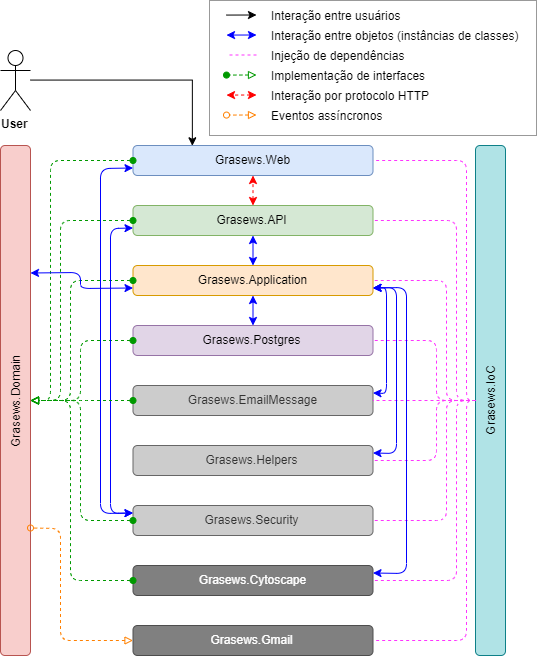
\includegraphics[scale=0.55]{4-grasews/imagens/grasews-architecture-simplified.png}
    \centering
    \caption[Arquitetura da ferramenta Grasews]{\textbf{Arquitetura da ferramenta Grasews.}}
    \label{fig:grasews-architecture-simplified}
\end{figure}

De forma resumida e simplificada, o fluxo da aplicação segue da seguinte forma: O usuário interage com o módulo \texttt{Grasews.Web}, o qual se comunica com \texttt{Grasews.API} por meio de requisições HTTP. Tanto \texttt{Grasews.Web} quanto \texttt{Grasews.API} utilizam funcionalidades providas por objetos de \texttt{Grasews.Security}. \texttt{Grasews.API} consome serviços providos por \texttt{Grasews.Application}, o qual orquestra o fluxo de trabalho conforme as regras de negócio da aplicação. Neste sentido, \texttt{Grasews.Application} é responsável por manipular objetos das entidades de domínio da aplicação juntamente com funcionalidades de apoio providas por \texttt{Grasews.Helpers}. Adicionalmente, \texttt{Grasews.Application} utiliza funcionalidades providas por \texttt{Grasews.Cytoscape}, para a manipulação de elementos do grafo, e funcionalidades providas por \texttt{Grasews.EmailMessage}, para a construção de mensagens de \textit{e-mail}. Juntamente com \texttt{Grasews.Gmail}, \texttt{Grasews.Application} invoca um evento assíncrono de \texttt{Grasews.Domain} para que a mensagem de \textit{e-mail}, previamente construída por \texttt{Grasews.EmailMessage}, seja enviada para um usuário. \texttt{Grasews.IoC} provê a injeção de dependências para todos os demais módulos da arquitetura.
\subsection{Interações Detalhadas entre Módulos de Grasews}\label{4-grasews-interacoes-detalhadas-modulos}

A \figurename~\ref{fig:grasews-architecture-detailed} detalha as principais interações dos módulos da arquitetura de Grasews. O fluxo da aplicação inicia-se com um usuário interagindo com a interface gráfica da aplicação por meio do módulo  \texttt{Grasews.Web} (à esquerda, na cor azul). \texttt{Grasews.Web} foi desenvolvido utilizando o padrão de arquitetura de desenvolvimento MVC e, portanto, seus principais componentes são representados por \texttt{Models}, \texttt{Views} e \texttt{Controllers}. Um usuário interage com um componente \texttt{View} que, por sua vez, utiliza um objeto modelo definido por um componente \texttt{Model}. A ações de um usuário resultam em eventos controlados por um componente \texttt{Controller}. O componente \texttt{Startup} é responsável por requisitar ao componente \texttt{SimpleInjectorBootstrap} o controle de dependências da aplicação. \texttt{SimpleInjectorBootstrap} (canto inferior, na cor ciano), do módulo \texttt{Grasews.IoC}, é responsável por criar um repositório de referências a objetos (classes) que serão necessários e utilizados por toda a aplicação. Estes objetos tornam-se disponíveis aos demais componentes da aplicação por meio da injeção de dependências realizada nos construtores destes demais componentes. Por fim, um componente de \texttt{Controller} utiliza o componente \texttt{RestClient} para que uma nova requisição seja feita à API da aplicação. O componente \texttt{RestClient} (canto superior, na cor vermelha) é provido pelo módulo \texttt{Grasews.Helpers} (canto superior, na cor cinza claro).

\begin{landscape}
    \begin{figure}[h]
        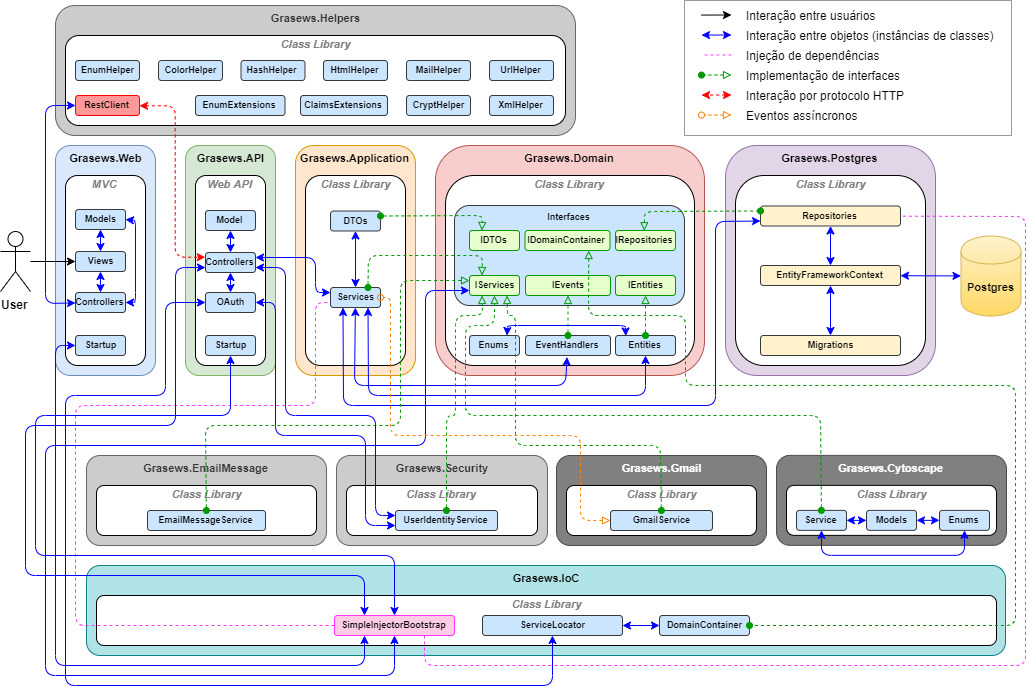
\includegraphics[scale=0.6]{4-grasews/imagens/grasews-architecture-detailed.png}
        \centering
        \caption[Arquitetura do Grasews de forma detalhada]{\textbf{Arquitetura do Grasews de forma detalhada.}}
        \label{fig:grasews-architecture-detailed}
    \end{figure}
\end{landscape}

A API da aplicação é provida pelo módulo \texttt{Grasews.API} (centro à esquerda, na cor verde). Os principais componentes deste módulo são os \texttt{Controllers} e os \texttt{Models}. As requisições originadas de \texttt{Grasews.Web} são gerenciadas por um \texttt{Controller} da API. Tais requisições são repassadas aos serviços do módulo \texttt{Grasews.Application}. Adicionalmente, \texttt{Grasews.API} contém o componente \texttt{Startup}, que assim como no módulo \texttt{Grasews.Web}, este componente é responsável por requisitar o registro de dependências ao módulo \texttt{Grasews.IoC}. Por fim, todos as requisições realizadas para \texttt{Grasews.API} são protegidas. Para realizar uma ação na ferramenta, o usuário deve ser autenticado pelo componente \texttt{OAuth}. Este componente é responsável por validar as credenciais de um usuário, permitindo o uso das funcionalidades da ferramenta, tanto por meio do módulo \texttt{Grasews.Web} quanto do módulo \texttt{Grasews.API}. O componente \texttt{OAuth} utiliza recursos providos por \texttt{UserIdentityService}, do módulo \texttt{Grasews.Security}, localizado no centro inferior do diagrama, na cor cinza claro. Adicionalmente, \texttt{OAuth} utiliza o componente \texttt{ServiceLocator} para obter instâncias de classes que ainda não foram introduzidas no contexto da aplicação pelo componente \texttt{SimpleInjectorBootstrap}. Isso ocorre pelo fato do componente \texttt{OAuth} ser instanciado no início do ciclo da vida da aplicação e não permitir que seu construtor tenha parâmetros de entrada, fator este que possibilita a injeção de dependências. \texttt{ServiceLocator} é auxiliado pelo componente \texttt{DomainContainer}, que atua como um repositório de objetos da aplicação.

O módulo \texttt{Grasews.Application} é representado simplificadamente por meio dos componentes \texttt{Services} e \texttt{DTOs} (\textit{Data Transfer Objects}). As classes que compõem os serviços (\texttt{Services}) são responsáveis por orquestrar todas as requisições originadas do módulo \texttt{Grasews.API}. Requisições realizadas ao módulo \texttt{Grasews.Application} resultam na utilização de objetos das camadas inferiores, como, por exemplo, a criação de instâncias de entidades de domínio, de \texttt{Grasews.Domain}, ou o consumo de métodos de classes de acesso a dados, denominados repositórios, de \texttt{Grasews.Postgres}. Os parâmetros de entrada e de saída de serviços do módulo \texttt{Grasews.Application} variam entre tipos simples, e.g., \textit{int} e \textit{string}, instâncias de entidades de domínio ou então instâncias de um \texttt{DTO}. Nenhum objeto de um tipo de \texttt{Model} de \texttt{Grasews.API} é transferido para \texttt{Grasews.Application}. Os \texttt{Controllers} de \texttt{Grasews.API} são responsáveis por converter seus objetos de tipos de  \texttt{Models} para objetos de tipo de uma entidade de domínio ou então de tipo de um \texttt{DTO}. Desta forma, obtém-se uma melhor segregação do escopo de objetos de cada módulo e, consequentemente, um maior desacoplamento entre os módulos, tornando um módulo o mais autossuficiente possível.

O módulo \texttt{Grasews.Domain} (centro, na cor salmão) contém todas as interfaces (na cor verde claro) de desenvolvimento que são implementadas pelos demais módulos da aplicação. Adicionalmente, \texttt{Grasews.Domain} é responsável por definir as entidades do domínio de negócio da aplicação, representadas pelo componente \texttt{Entities} (na cor azul). Uma entidade geralmente representa uma tabela no banco de dados. Por meio do módulo \texttt{Grasews.Postgres}, estas entidades e suas propriedades são mapeadas para tabelas e colunas do banco de dados, respectivamente. Por fim, \texttt{Grasews.Domain} possui componentes responsáveis por controlar eventos assíncronos. Eventos assíncronos são funcionalidades que podem ser executadas independentemente do fluxo da aplicação, pois não geram dependências para a aplicação. Por exemplo, o envio de um \textit{e-mail} para um usuário pode ser executado de forma assíncrona. Os componentes responsáveis pela implementação do controle de eventos assíncronos são os \texttt{EventHandlers} e as interfaces de \texttt{IEvents}.

O módulo \texttt{Grasews.Postgres} (centro à esquerda, na cor lilás) é responsável por realizar o acesso da aplicação ao banco de dados. Seus principais componentes são os repositórios (\texttt{Repositories}) e o contexto do banco de dados implementado pelo uso do \textit{Microsoft Entity Framework}. O contexto do banco de dados é representado por \texttt{EntityFrameworkContext}. Todas as ações executadas em Grasews que necessitam acesso ao banco de dados são realizadas pelos repositórios. Os repositórios implementam interfaces definidas no módulo \texttt{Grasews.Domain}. Grasews utiliza o SGBD \textit{Postgres} (centro à esquerda, na cor amarelo). Adicionalmente, toda a estrutura de banco de dados de Grasews foi gerada automaticamente por meio do componente \texttt{Migrations} com base nas classes de entidades de domínio existentes no módulo \texttt{Grasews.Domain}. \texttt{Migrations} permite que alterações no modelo do código sejam feitas e depois sejam propagadas no banco de dados.

O módulo \texttt{Grasews.Helpers} (canto superior, na cor cinza claro) possui componentes com funcionalidades que dão suporte a todos os demais módulos de Grasews. Este módulo é composto por diversos componentes com variados propósitos a fim de auxiliar demais objetos da arquitetura da ferramenta. Por fim, o módulo \texttt{Grasews.Cytoscape} (canto inferior direito, na cor cinza escuro) é responsável por manipular nós e arestas do grafo de Grasews. Este módulo foi desenvolvido baseado nas funcionalidades e modelos necessários da biblioteca de desenvolvimento \texttt{Cytoscape.js}, utilizada pelo módulo \texttt{Grasews.Web} para o desenvolvimento dos grafos na interface gráfica de usuário da ferramenta. Os principais componentes de \texttt{Grasews.Cytoscape} são \texttt{Service}, contendo os métodos para manipulação dos elementos (modelos) do grafo, e \texttt{Models}, contendo os tipos de dados necessários para a representação de elementos no grafo, como, por exemplo, nós, arestas e propriedades visuais.
\section{Visão Geral da Implementação}\label{4-grasews-visao-geral-implementacao}

O módulo de \textit{front-end} foi desenvolvido seguindo a arquitetura MVC provido pelo \textit{ASP.NET MVC}~\cite{MICROSOFT-2019-ASP-NET-MVC}. Neste módulo, a biblioteca \textit{jQuery}~\cite{JQUERY-2019} foi intensivamente utilizada em conjunto com a linguagem \textit{JavaScript} para o desenvolvimento de funcionalidades do lado cliente para o módulo de \textit{front-end}. Adicionalmente, para a formatação da interface gráfica de usuário de Grasews, as linguagens HTML5 e CSS3 foram utilizadas, ambas suportadas por \textit{templates} providos por \textit{Admin LTE}~\cite{ADMIN-LTE-2019}, por funcionalidades providas por \textit{Bootstrap}~\cite{BOOTSTRAP-2019} e por ícones providos por \textit{Font-Awesome}~\cite{FONT-AWESOME-2019}.

O formato padrão de comunicação entre o \textit{front-end} e o \textit{back-end} é o formato JSON~\cite{JSON-2019}. Neste sentido, todas as mensagens utilizadas nas interações entre os a interface de usuário e a API da aplicação utilizam objetos JSON. Adicionalmente, o formato JSON é utilizado na criação dos grafos da ferramenta, provido pela biblioteca \textit{Cytoscape.js}\cite{CYTOSCAPE-2015}.

As principais linguagens de programação utilizadas no desenvolvimento da ferramenta Grasews foi o linguagem C\#, do \textit{framework} .NET~\cite{MICROSOFT-2019-NET-FRAMEWORK}. C\# possibilitou o desenvolvimento de funcionalidades do lado servidor providas pelos módulos de \textit{back-end} da aplicação. A API da aplicação foi desenvolvida como serviços web RESTful, suportados pelo \textit{ASP.NET Web API}~\cite{MICROSOFT-2019-WEB-API}. Adicionalmente, a utilização do ORM \textit{.NET Entity Framework}~\cite{MICROSOFT-2019-Entity-Framework} possibilitou uma mais fácil implementação do mapeamento de classes .NET para tabelas do banco de dados, bem como na criação da estrutura do banco de dados (\textit{migrations}) e na persistência de dados da aplicação no \textit{Postgres}~\cite{POSTGRES-2019}.

Um conjunto de ferramentas foi utilizado no desenvolvimento de Grasews. A seguir, são listadas as principais ferramentas que deram suporte ao desenvolvimento de Grasews.

\begin{enumerate}

  \item \textbf{Microsoft Visual Studio 2017 e 2019}
  
  \textit{Microsoft Visual Studio} é um ambiente (IDE) de desenvolvimento para linguagens de programação do \textit{framework} .NET, entre outras. \textit{Visual Studio} provê fácil integração com \textit{Microsoft Azure} e com \textit{Microsoft Azure DevOps}, para publicação de aplicações e controle de versão do código-fonte, respectivamente. Todos os módulos de Grasews foram desenvolvidos utilizando o \textit{Visual Studio}.
  
  %Para mais informações, consulte \href{https://visualstudio.microsoft.com/}{https://visualstudio.microsoft.com/}
  
  \item \textbf{pgAdmin}
  
 \textit{pgAdmin}~\cite{PGADMIN-2019} é a plataforma de administração e desenvolvimento mais popular e com mais recursos para o banco de dados \textit{PostgreSQL}. Assim como \textit{PostgreSQL}, \textit{pgAdmin} é desenvolvido com o códio aberto. Durante o desenvolvimento de Grasews, a fim de validar os
  
  %Para mais informações, consulte \href{https://www.pgadmin.org/}{https://www.pgadmin.org/}
  
  \item \textbf{Postman}
  
  \textit{Postman}~\cite{POSTMAN-2019} é uma plataforma de colaboração para o desenvolvimento de APIs. Os recursos do \textit{Postman} simplificam cada etapa da criação de uma API e agilizam a colaboração para que você possa criar APIs mais rapidamente. Utilizamos \textit{Postman} para validar as funcionalidades disponíveis em \texttt{Grasews.API}, bem como para agilizar o uso da ferramenta de uma perspectiva do desenvolvimento. Uma coleção de requisições para \texttt{Grasews.API} foi criada e salva \textit{Postman} Com isso, podemos validar tanto os endereços dos \textit{endpoints}, quanto os parâmetros de entrada e as respostas dos \textit{endpoints}.
  
  %Para mais informações, consulte \href{https://www.getpostman.com/}{https://www.getpostman.com/}
  
  \item \textbf{Microsoft Azure Hosting}
  
  \textit{Microsoft Azure}~\cite{MICROSOFT-2019-AZURE} é um serviço de computação em nuvem criado por \textit{Microsoft} para criar, testar, implantar e gerenciar aplicativos e serviços por meio de data centers gerenciados por \textit{Microsoft}. Utilizamos \textit{Microsoft Azure} para hospedar tanto \texttt{Grasews.Web} quanto \texttt{Grasews.API}. O endereço web de \texttt{Grasews.Web} é  \href{https://grasewsweb.azurewebsites.net/}{https://grasewsweb.azurewebsites.net/} e de \texttt{Grasews.API} é  \href{https://grasewsapi.azurewebsites.net/}{https://grasewsapi.azurewebsites.net/}.
  
  %Para mais informações, consulte \href{https://azure.microsoft.com/}{https://azure.microsoft.com/}
  
  \item \textbf{Microsoft Azure DevOps}
  
  \textit{Microsoft Azure DevOps}~\cite{MICROSOFT-2019-DEVOPS} é um repositório de código-fonte oferecido por \textit{Microsoft}. Por meio de \textit{Microsoft Azure DevOps}, desenvolvedores podem versionar o código-fonte, bem como controlar as entregas e automatizar tarefas como compilações e publicações de aplicações. Todo o código-fonte de Grasews está controlado por meio de \textit{Microsoft Azure DevOps}. O endereço web do repositório é \href{https://dev.azure.com/matheuscalache/Grasews}{https://dev.azure.com/matheuscalache/Grasews}.
  
  %Para mais informações, consulte \href{https://azure.microsoft.com/en-us/services/devops/}{https://azure.microsoft.com/en-us/services/devops/}
  
\end{enumerate}

A \figurename~\ref{fig:grasews-technology-stack} apresenta a pilha de tecnologias utilizada na arquitetura de desenvolvimento do Grasews. No topo, encontramos as tecnologias utilizadas para o desenvolvimento da camada de \textit{front-end} de Grasews, i.e., a interface gráfica de usuário. Nesta camada, à esquerda encontramos as principais tecnologias utilizadas do \textit{framework} .NET. Ao centro da camada de \textit{front-end}, encontramos as principais tecnologias e bibliotecas utilizadas para o desenvolvimento com base na linguagem \textit{JavaScript}. Por fim, acima das bibliotecas \textit{JavaScript}, encontramos as principais tecnologias e bibliotecas utilizadas para formatação e apresentação de páginas web (HTML e CSS). Abaixo da camada de \textit{front-end}, são representadas as principais tecnologias utilizadas para o desenvolvimento da camada de \textit{back-end}. Nesta camada utilizamos exclusivamente tecnologias do \textit{framework} .NET. A próxima camada é a camada de persistência de dados. Nesta camada, encontramos o uso do banco de dados Postgres. Por fim, a camada na base da figura apresenta a plataforma de hospedagem e controle de código-fonte, provida pela solução em nuvem \textit{Microsoft Azure}.

O Apêndice \ref{apendice-tecnologias-grasews} apresenta uma visão geral das principais tecnologias e bibliotecas de desenvolvimento utilizadas na implementação de Grasews.

\begin{landscape}
    \begin{figure}[h]
        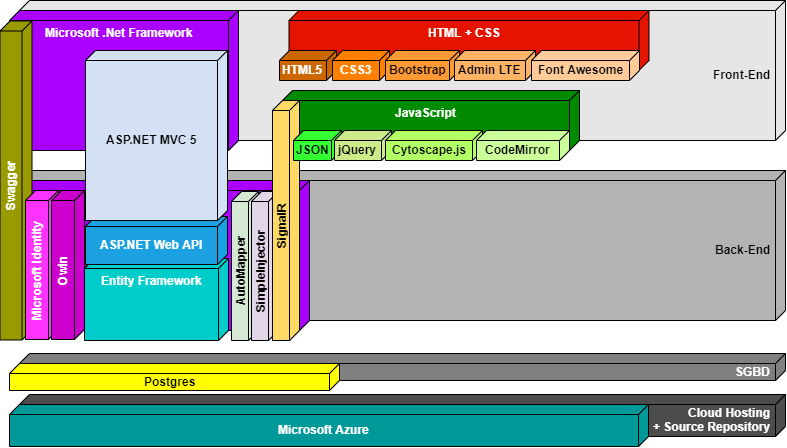
\includegraphics[scale=0.7]{4-grasews/imagens/grasews-technology-stack.png}
        \centering
        \caption[Pilha de tecnologias envolvidas no desenvolvimento do Grasews]{\textbf{Pilha de tecnologias envolvidas no desenvolvimento do Grasews.}}
        \label{fig:grasews-technology-stack}
    \end{figure}
\end{landscape}
\section{Suporte à Anotação Semântica}\label{4-grasews-suporte-anotacao}

Grasews provê recursos para que o usuário seja capaz de anotar semanticamente uma especificação WSDL. Por meio de menus de contexto, o usuário é capaz de criar anotações utilizando tanto o atributo \textit{Model Reference} quanto os atributos \textit{Lifting Schema Mapping} e \textit{Lowering Schema Mapping}, do padrão SAWSDL.

A \figurename~\ref{fig:grasews} ilustra a interface gráfica de Grasews, contendo os três principais componentes visuais de Grasews. Ao centro, encontra-se o painel de visualização tanto do grafo quanto do código WSDL/XML, apresentado na seção \ref{4-grasews-grafo}. À esquerda, encontra-se o painel de visualização de elementos de uma especificação WSDL no formato de menu de árvore (\textit{tree-view}), apresentado na seção \ref{4-menu-wsdl}. Por fim, à direita, encontra-se o painel de visualização de classes de uma ontologia OWL também no formato de menu de árvore (\textit{tree-view}), apresentado na seção \ref{4-menu-owl}.

\subsection{Grafo com Suporte à Anotação Semântica}\label{4-grasews-grafo}

O principal componente visual de Grasews é o grafo. Grasews utiliza a notação visual proposta no Capítulo \ref{3-notacao-visual-para-sawsdl} para representar hierarquicamente elementos de uma especificação WSDL e classes de uma ontologia OWL, possibilitando que um usuário crie anotações semânticas segundo a abordagem SAWSDL. Para os elementos WSDL/XSD passíveis de serem anotados com \textit{Model Reference}, Grasews disponibiliza um menu de contexto para adicionar e remover um URI de \textit{Model Reference}. Para os elementos passíveis de serem anotados tanto com \textit{Model Reference} quanto com \textit{Lifting Schema Mapping} e \textit{Lowering Schema Mapping}, Grasews estende o menu de contexto anterior com opções adicionais para permitir todos os tipos de anotações. A \figurename~\ref{fig:grasews-grafo-tipo-complexo-contexto} ilustra o menu de contexto disponível para um tipo complexo XSD \texttt{GetAllBooks} (parcialmente visível atrás do menu de contexto).

A \figurename~\ref{fig:grasews-grafo-model-reference} apresenta parte do grafo de uma especificação WSDL anotada com \textit{Model Reference}. Observa-se que a interface \texttt{MyWebSerice} está anotada com \textit{Model Reference} utilizando a classe OWL \texttt{ExpressionContent}, esta pertencente à ontologia \texttt{books}. Adicionalmente, a operação \texttt{MyMethodB} está anotada com \textit{Model Reference} utilizando a classe OWL \texttt{Article}, da mesma ontologia. Grasews constrói automaticamente a estrutura hierárquica entre as duas classes OWL em uso por anotações semânticas. Com isso, as classes OWL intermediárias \texttt{LinguisticExpression} e \texttt{Text} são automaticamente dispostas no grafo entre as duas classes OWL \texttt{ExpressionContent} e \texttt{Article}.

\begin{landscape}
    \begin{figure}[h]
        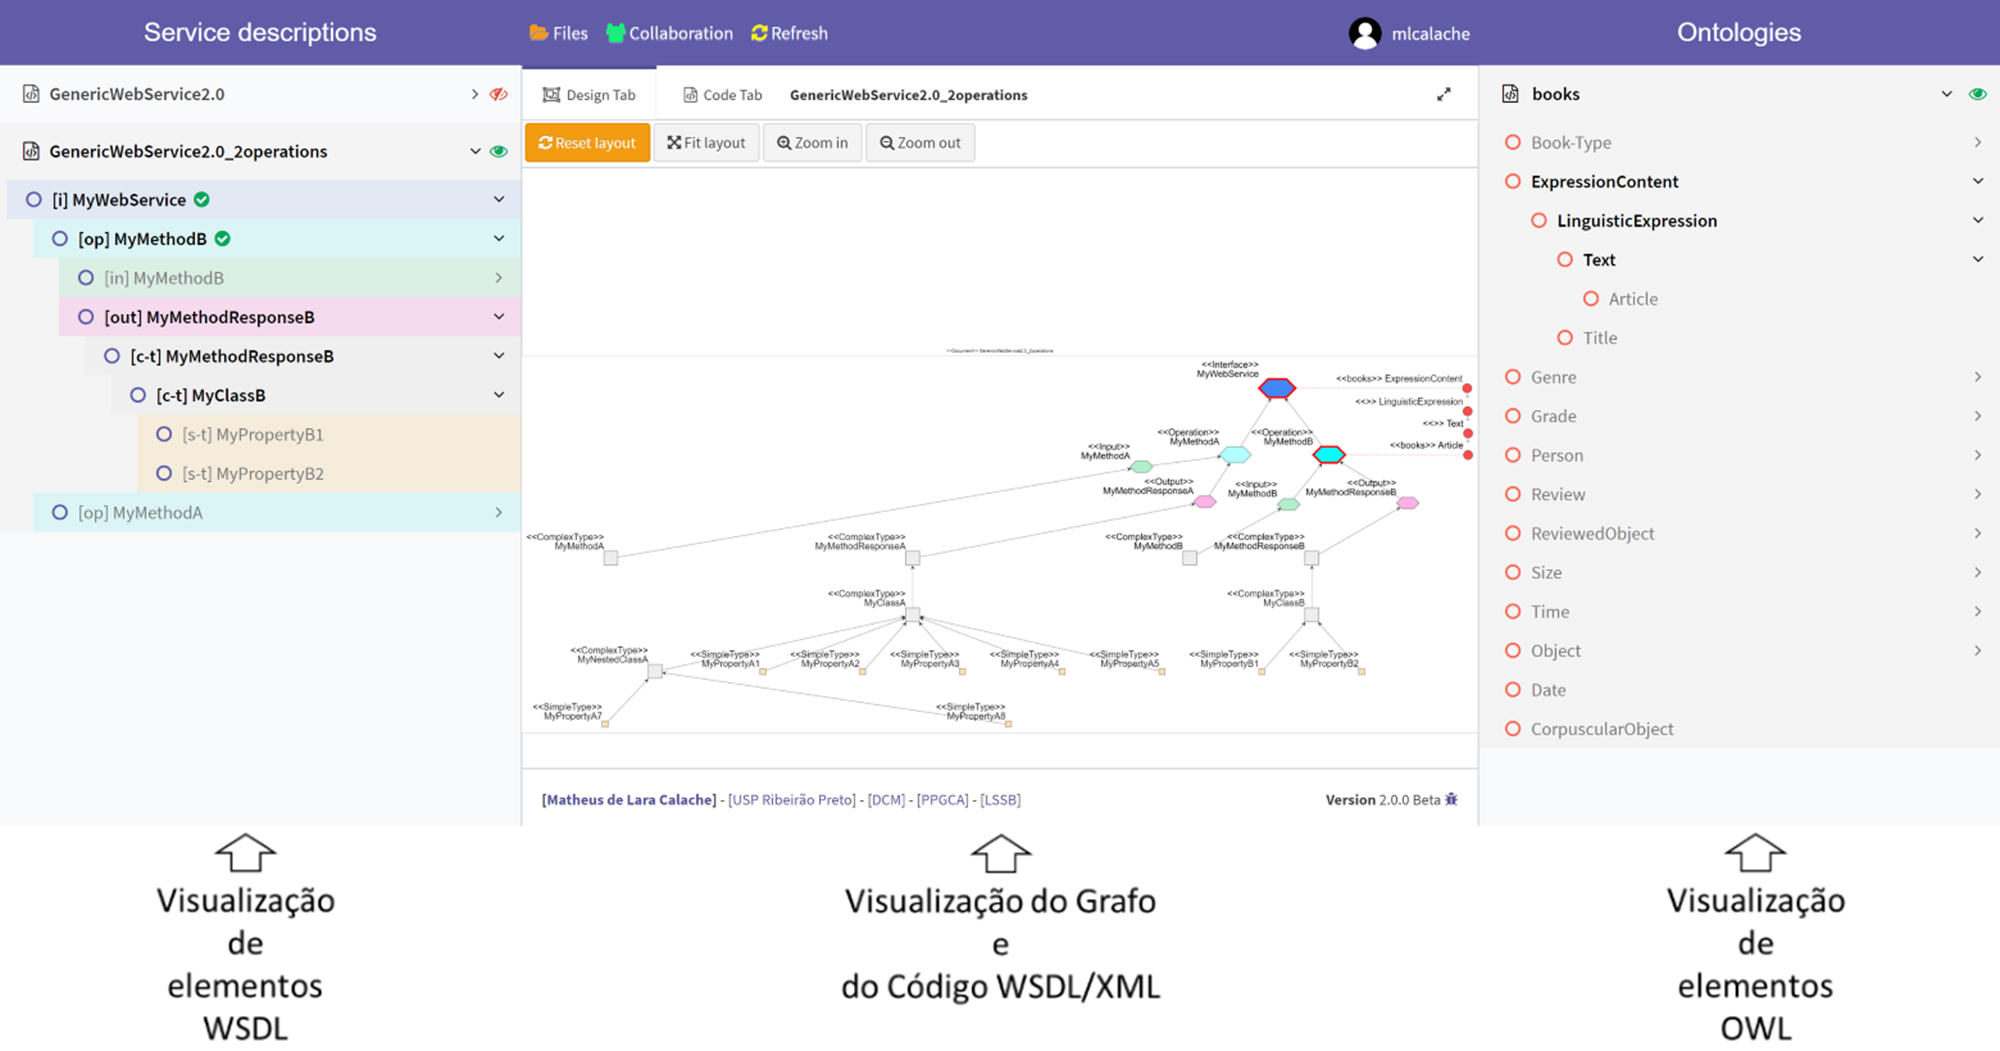
\includegraphics[scale=0.45]{4-grasews/imagens/grasews.png}
        \centering
        \caption[Interface gráfica de Grasews]{\textbf{Interface gráfica de Grasews.}}
        \label{fig:grasews}
    \end{figure}
\end{landscape}

Adicionalmente, Grasews provê um painel para visualizar o código XML de uma especificação WSDL. A \figurename~\ref{fig:grasews-painel-codigo} ilustra o painel de visualização do código WSDL/XML. O painel é automaticamente atualizado conforme o trabalho (anotações semânticas) é realizado. Com isso, caso o usuário tenha conhecimento técnico no código XML de uma especificação WSDL, este usuário pode verificar o painel de código a fim de validar as anotações semânticas criadas com o auxílio das notações visuais de Grasews. Entretanto, o painel de visualização de código não é editável.

\begin{figure}[h]
    %\resizebox{\textwidth}{!}{
        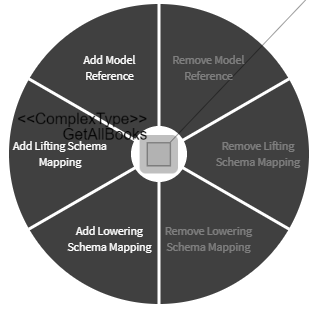
\includegraphics[scale=0.8]{4-grasews/imagens/grasews-grafo-tipo-complexo-contexto.png}
    %}
    \centering
    \caption[Menu de contexto para anotação semântica por meio do grafo de Grasews]{\textbf{Menu de contexto para anotação semântica por meio de grafo do Grasews.}}
    \label{fig:grasews-grafo-tipo-complexo-contexto}
\end{figure}

\begin{figure}[h]
    \resizebox{\textwidth}{!}{
        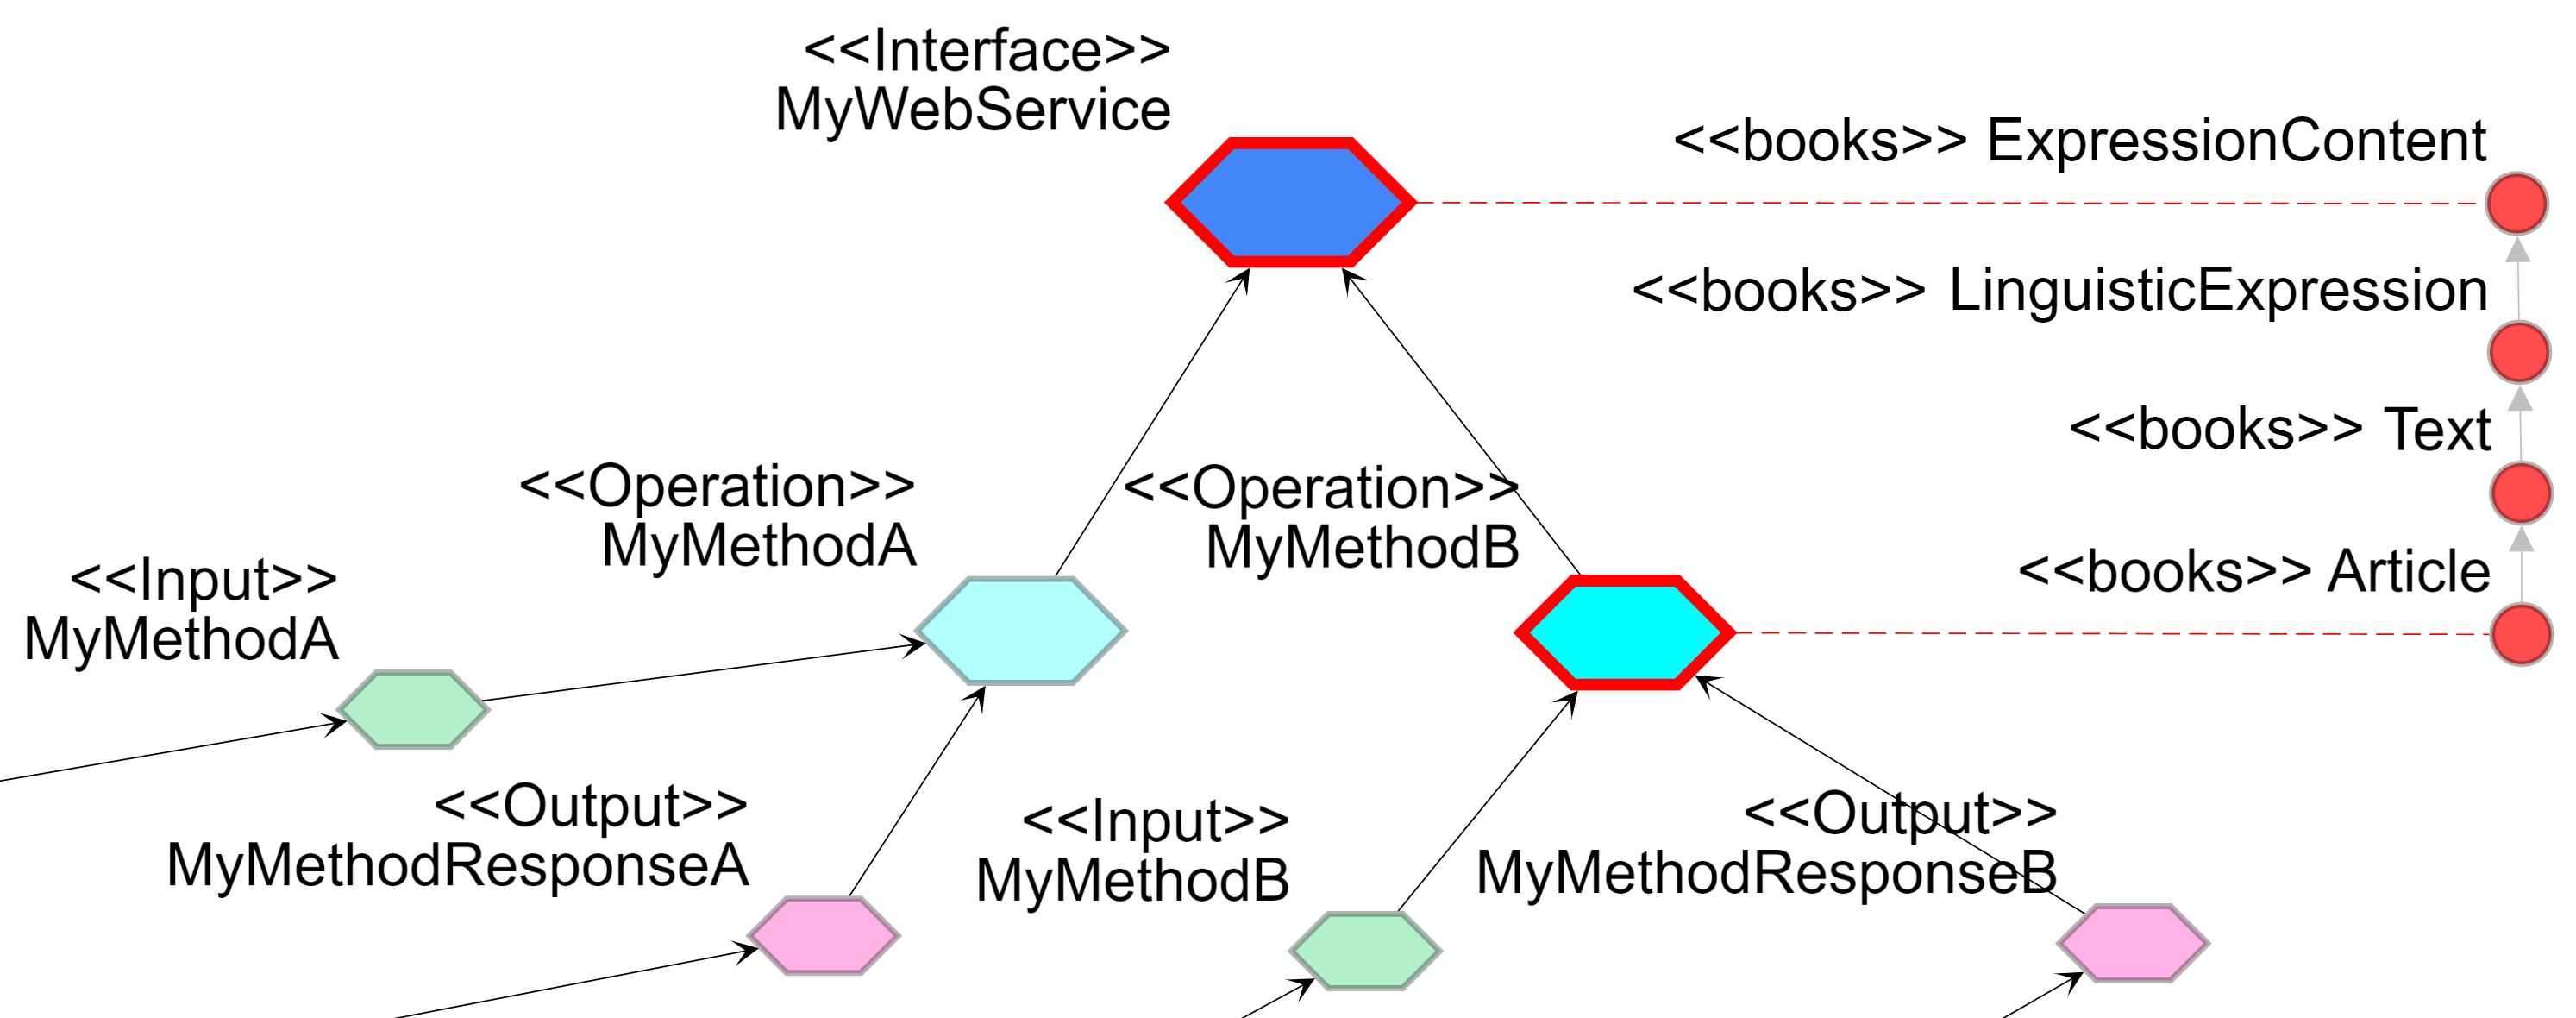
\includegraphics[scale=0.8]{4-grasews/imagens/grasews-grafo-model-reference.png}
    }
    \centering
    \caption[Elementos do grafo de Grasews anotados com \textit{Model Reference}]{\textbf{Elementos do grafo de Grasews anotados com \textit{Model Reference}.}}
    \label{fig:grasews-grafo-model-reference}
\end{figure}

\begin{figure}[h]
    \resizebox{\textwidth}{!}{
        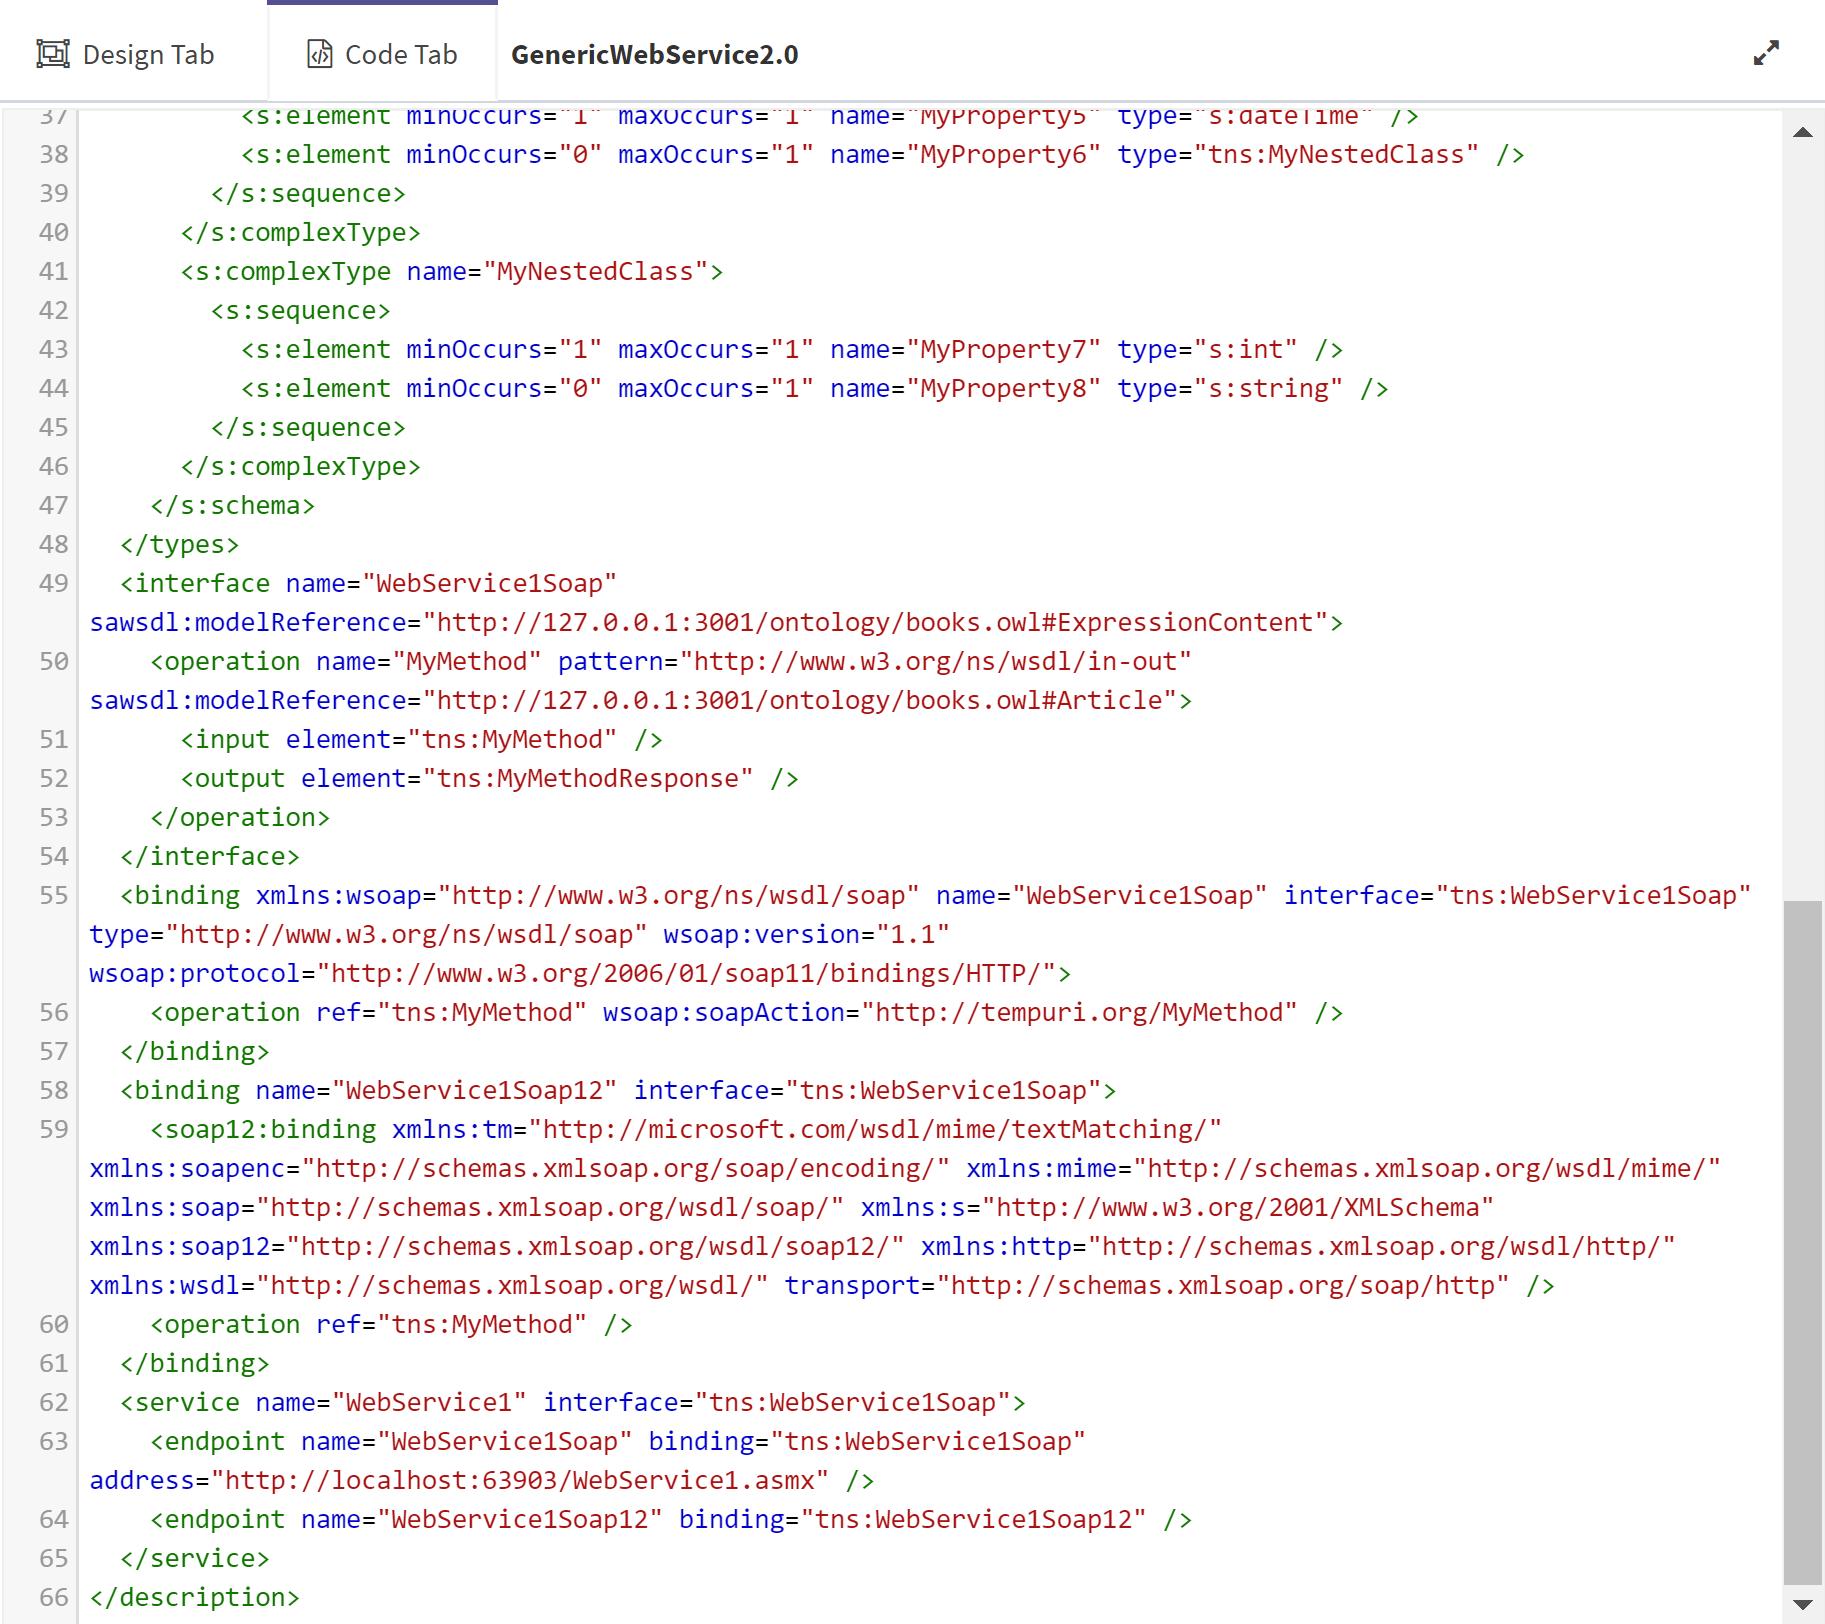
\includegraphics[scale=0.250]{4-grasews/imagens/grasews-painel-codigo.png}
    }
    \centering
    \caption[Painel de Grasews para visualização do código WSDL/XML]{\textbf{Painel de Grasews para visualização do código WSDL/XML.}}
    \label{fig:grasews-painel-codigo}
\end{figure}
\section{Menu \textit{tree-view}}\label{4-grasews-menu-tree-view}

Grasews utiliza um menu no formato de árvore (\textit{tree-view}) para auxiliar na compreensão tanto de uma especificação WSDL quanto de uma ontologia OWL, facilitando, consequentemente, o processo de anotação semântica.

\input{4-grasews/4.3.2.1-menu-wsdl.tex}
\input{4-grasews/4.3.2.3-menu-owl.tex}
\section{Suporte à Edição Colaborativa}\label{4-grasews-suporte-edicao-colaborativa}

Grasews provê suporte para a anotação semântica de forma colaborativa, ou seja, múltiplos usuários podem simultaneamente anotar semanticamente uma especificação WSDL. Esta seção apresenta uma visão geral de como Grasews provê o suporte para a anotação semântica de forma colaborativa.

\subsection{Anotação Semântica Colaborativa}\label{4-edicacao-semantica-colaborativa}

Por meio do menu de colaboração, um usuário pode compartilhar o seu projeto com outros usuários. Um projeto refere-se às especificações WSDL juntamente com as ontologias OWL abertas na ferramenta. O primeiro passo para o trabalho colaborativo é compartilhar o projeto com outro usuário. Grasews disponibiliza um menu com funcionalidades relacionadas à edição colaborativa. Um usuário de Grasews pode convidar outro usuário para o trabalho colaborativo. O usuário convidado pode ser tanto um novo usuário quanto um usuário já existente. O usuário convidado receberá um \textit{e-mail} que permitirá que ele aceite ou negue o convite para a edição colaborativa. Caso seja um novo usuário e aceite o convite, Grasews solicitará que realize o cadastro na ferramenta. Tendo aceito o convite, após autenticar-se na ferramenta, o usuário poderá abrir a especificação WSDL e as ontologias OWL compartilhadas com ele, da mesma forma como se tivesse sido este usuário que houvesse carregado estes documentos na ferramenta.

Uma vez com a especificação WSDL aberta no sistema, múltiplos usuários podem anotar semanticamente o documento. A partir deste ponto, todo o trabalho realizado é compartilhado e simultaneamente disponibilizado aos demais usuários que estão com a mesma especificação WSDL aberta na ferramenta. Caso haja outros usuários autenticados e com a mesma especificação WSDL aberta na ferramenta, por meio do compartilhamento da especificação, o projeto destes usuários é automaticamente atualizado, trazendo as edições recentemente realizadas na especificação WSDL. Desta forma, o grafo e o menu \textit{tree-view} são automaticamente atualizados de forma a representarem a última versão da especificação WSDL compartilhada. De modo a facilitar o trabalho colaborativo e remoto, Grasews provê um conjunto de notificações que são disparadas aos usuários conforme o trabalho é realizado. Tais notificações aparecem no canto inferior direito da ferramenta.

A \figurename~\ref{fig:grasews-anotacao-semantica-compartilhada} ilustra um caso de uso durante o processo de anotação semântica de forma colaborativa. À esquerda, encontram-se os estados do ambiente de trabalho de um \texttt{Usuário A}, enquanto que à direita encontram-se os ambientes de trabalho de um \texttt{Usuário B}. A \figurename~\ref{fig:grasews-anotacao-semantica-compartilhada}a e a \figurename~\ref{fig:grasews-anotacao-semantica-compartilhada}b ilustram os ambientes de trabalho do \texttt{Usuário A} e do \texttt{Usuário B}, respectivamente, em seus estados iniciais. A \figurename~\ref{fig:grasews-anotacao-semantica-compartilhada}c ilustra o ambiente de trabalho do \texttt{Usuário A} após este ter adicionado um \textit{Model Reference} ao elemento tipo complexo \texttt{MyMethodResponseB}, na lateral direita do grafo. Simultaneamente, a \figurename~\ref{fig:grasews-anotacao-semantica-compartilhada}d ilustra o ambiente de trabalho do \texttt{Usuário B} com o mesmo estado inicial, pois a nova anotação semântica ainda não foi notificada ao \texttt{Usuário B}. A \figurename~\ref{fig:grasews-anotacao-semantica-compartilhada}e ilustra o ambiente de trabalho do \texttt{Usuário A} com a anotação semântica feita anteriormente. Finalmente, a \figurename~\ref{fig:grasews-anotacao-semantica-compartilhada}f ilustra o ambiente de trabalho do \texttt{Usuário B} após receber a notificação e a atualização com a anotação semântica criada pelo \texttt{Usuário A} anteriormente.

%\begin{landscape}
    \begin{figure}[h!]
        %\resizebox{\textwidth}{!}{
            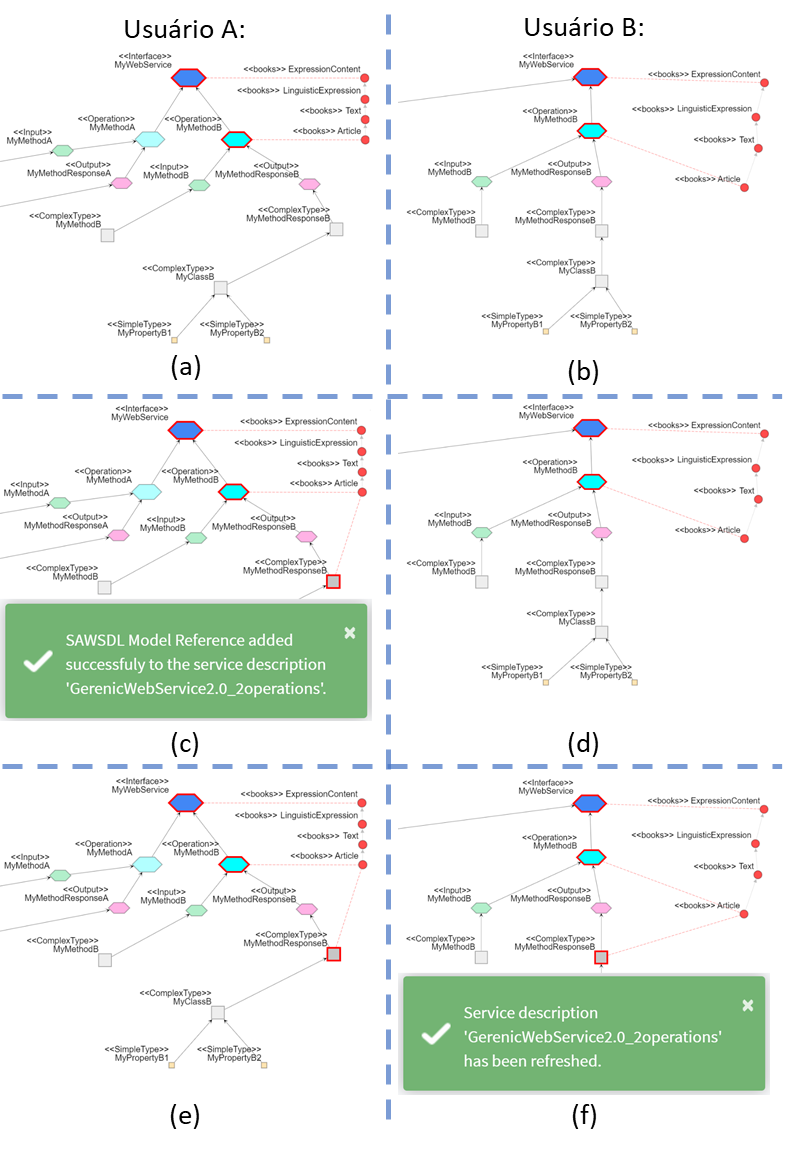
\includegraphics[scale=0.66]{4-grasews/imagens/grasews-anotacao-semantica-compartilhada.png}
        %}
        \centering
        \caption[Processo de anotação semântica de forma colaborativa de Grasews]{\textbf{Processo de anotação semântica de forma colaborativa de Grasews.} (a) Estado inicial de \texttt{Usuário A}. (b) Estado inicial de \texttt{Usuário B}. (c) \texttt{Usuário A} adiciona uma anotação semântica. (d) \texttt{Usuário B} ainda com estado inicial. (e) Estado final de \texttt{Usuário A} com a nova anotação semântica. (f) \texttt{Usuário B} recebe notificação e atualização com a nova anotação semântica.}
        \label{fig:grasews-anotacao-semantica-compartilhada}
    \end{figure}
%\end{landscape}

De forma a evitar inconsistências nas edições colaborativas de uma especificação WSDL, Grasews controla o trabalho colaborativo por meio dos módulos \texttt{Grasews.Application} e \texttt{Grasews.Postgres}. \texttt{Grasews.Application} garante que requisições de anotações semânticas, criadas pelo módulo \texttt{Grasews.API}, sejam verificadas e validadas juntamente com o \texttt{Grasews.Postgres} a fim de que um usuário não sobrescreva o trabalho de outro usuário por conta de requisições concorrentes. Assim, caso haja requisições concorrentes para a anotação de um mesmo elemento WSDL/XSD, apenas a primeira requisição recebida será processada, enquanto que as demais serão descartadas. Todos os usuários que criaram anotações semânticas de forma concorrente recebem notificações da ferramenta com os resultados de suas requisições, sejam os resultados de sucesso ou não. Entretanto, caso requisição seja descartada para um dado usuário, este pode remover anotações que foram realizadas por ele e por outros usuários e, então, adicionar novas anotações na especificação WSDL.

Por fim, cada usuário que possui uma especificação WSDL compartilhada com outros usuário pode reposicionar os nós do grafo individualmente. Grasews permite que cada usuário salve o seu próprio grafo com os ajustes (reposicionamentos) realizados. Este recurso também possibilita que cada usuário possa realizar a anotação semântica de forma personalizada, já que cada usuário pode ter uma forma diferente de compreender do grafo. Entretanto, as anotações realizadas na especificação e, consequentemente, as notações visuais do grafo são automaticamente compartilhadas, independentemente das posições dos nós do grafo. Note que na \figurename~\ref{fig:grasews-anotacao-semantica-compartilhada}, as posições dos nós do grafo do \texttt{Usuário A}, à esquerda, diferem das posições dos nós do grafo do \texttt{Usuário B}, à direita.
\subsection{Questões \& Tarefas}

O processo de anotação semântica colaborativo é auxiliado por meio da definição de questões e tarefas. Quando um usuário possui algum dúvida específica em relação a anotação de um elemento de uma especificação WSDL, este usuário pode criar uma questão (\textit{issue}) associada ao elemento. Uma questão não é direcionada a um usuário específico, i.e., qualquer usuário envolvido na edição colaborativa é capaz de visualizar as questões para uma especificação WSDL e respondê-las. É possível ter múltiplas respostas de múltiplos usuários. Quando uma questão é considerada devidamente respondida, o usuário que a criou pode marcá-la como resolvida. A \figurename~\ref{fig:grasews-lista-issues} ilustra a interface gráfica de Grasews para a listagem de questões. Por meio desta interface gráfica, um usuário pode adicionar respostas às questões e marcá-las como resolvidas.

\begin{figure}[h]
    %\resizebox{\textwidth}{!}{
        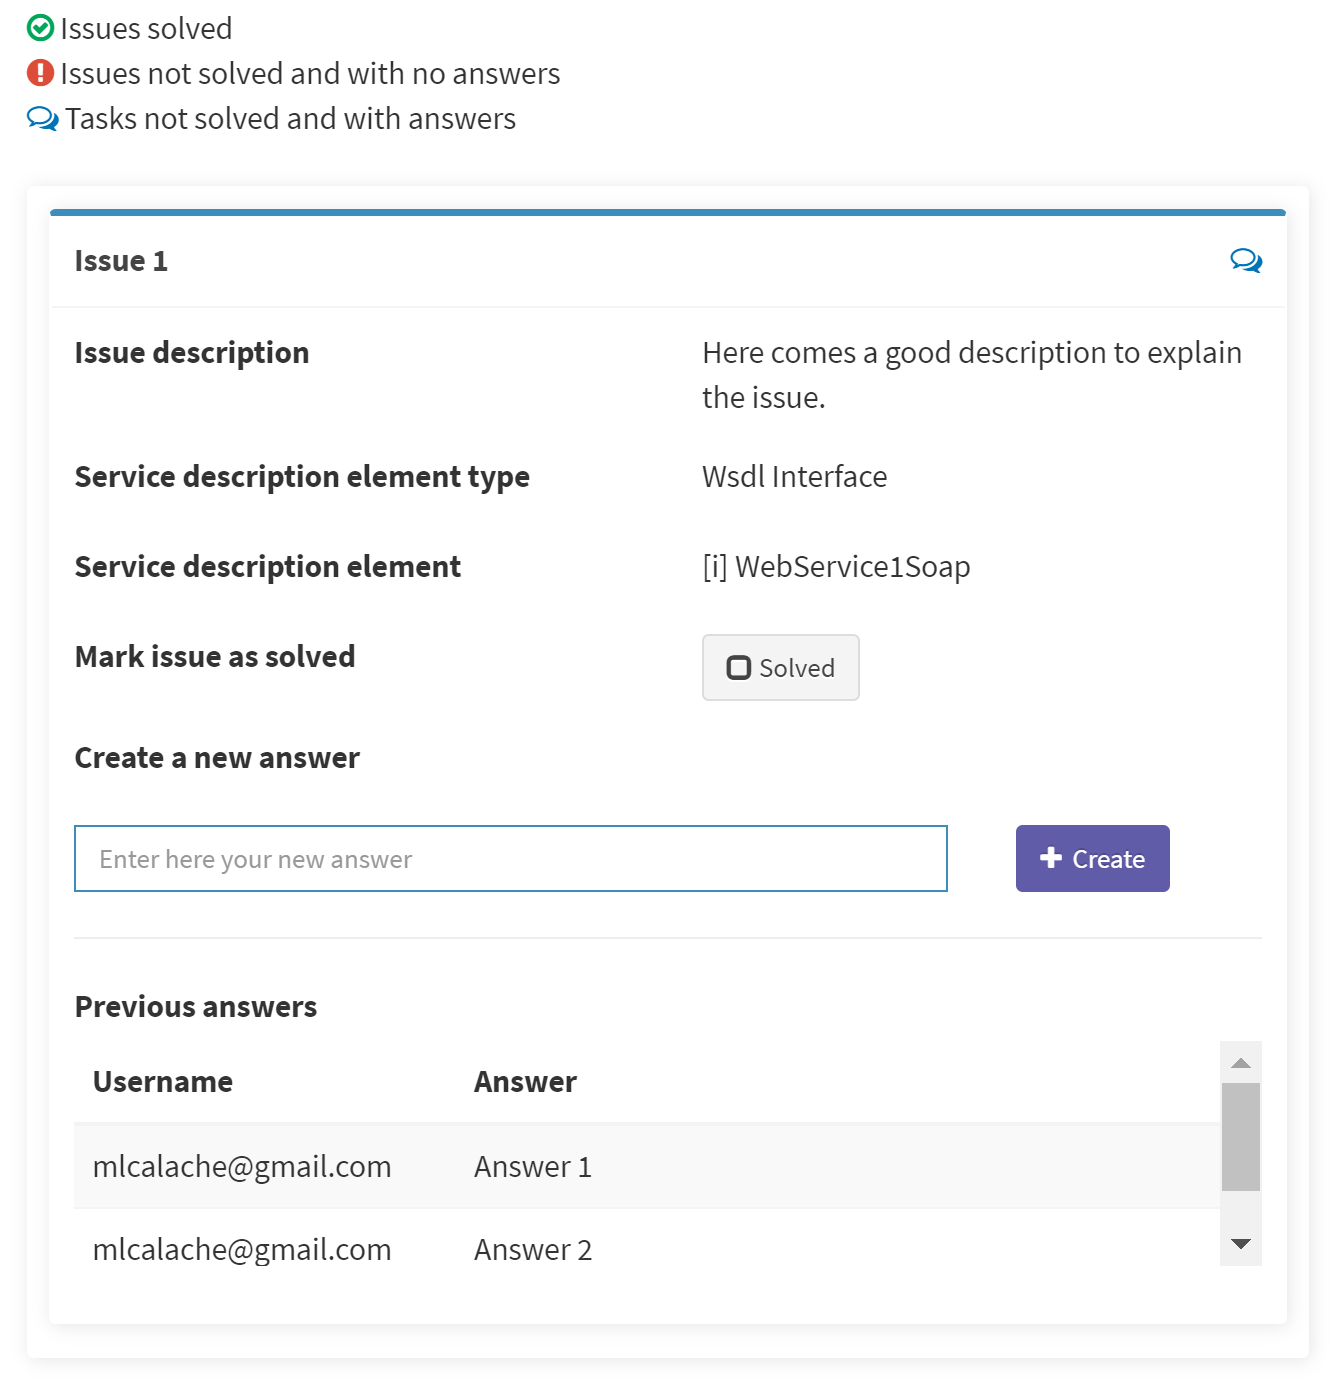
\includegraphics[scale=0.25]{4-grasews/imagens/grasews-lista-issues.png}
    %}
    \centering
    \caption[Interface gráfica para a lista de questões]{\textbf{Interface gráfica para a lista de questões.}}
    \label{fig:grasews-lista-issues}
\end{figure}

%Caso o usuário que criou a questão julgar que esta foi já propriamente respondida, este usuário pode marcar a questão como resolvida. Caso um elemento WSDL/XSD tenha todas as suas questões resolvidas, a representação visual deste elemento no grafo é automaticamente atualizada. Com isso, o elemento WSDL/XSD deixará de ser representado na cor amarela, conforme a notação visual proposta por este trabalho.

Quando um elemento WSDL/XSD possui uma questão não resolvida, o grafo WSDL de Grasews representa visualmente este elemento na cor amarela, substituindo, portanto, a cor original deste elemento. Caso o elemento WSDL/XSD não possua mais questões relacionadas, este elemento é representado em sua cor original conforme a notação visual proposta por este trabalho.

A \figurename~\ref{fig:grasews-anotacao-semantica-compartilhada-com-questoes} ilustra diferentes notações visuais envolvendo a anotação semântica de forma colaborativa e auxiliada por questões. A especificação WSDL exemplificada pela  \figurename~\ref{fig:grasews-anotacao-semantica-compartilhada-com-questoes} está compartilhada entre dois usuários: \texttt{Usuário A} e \texttt{Usuário B}. A \figurename~\ref{fig:grasews-anotacao-semantica-compartilhada-com-questoes}a ilustra a interface \texttt{MyWebService} para ambos os usuários em seu estado inicial, sem \textit{Model Reference} e sem questão. A \figurename~\ref{fig:grasews-anotacao-semantica-compartilhada-com-questoes}b ilustra a interface \texttt{MyWebService} com uma questão adicionada pelo \texttt{Usuário A}. O \texttt{Usuário B} responde esta questão, que auxiliou o \texttt{Usuário A} a anotar este elemento. A \figurename~\ref{fig:grasews-anotacao-semantica-compartilhada-com-questoes}c ilustra a interface \texttt{MyWebService} anotada e ainda com a questão. Finalmente, após ter realizada a anotação semântica, o \texttt{Usuário A} marca a sua questão como resolvida. A \figurename~\ref{fig:grasews-anotacao-semantica-compartilhada-com-questoes}d ilustra, portanto, a notação visual deste elemento, agora com \textit{Model Reference} e sem questão. 

\begin{figure}[h]
    %\resizebox{\textwidth}{!}{
        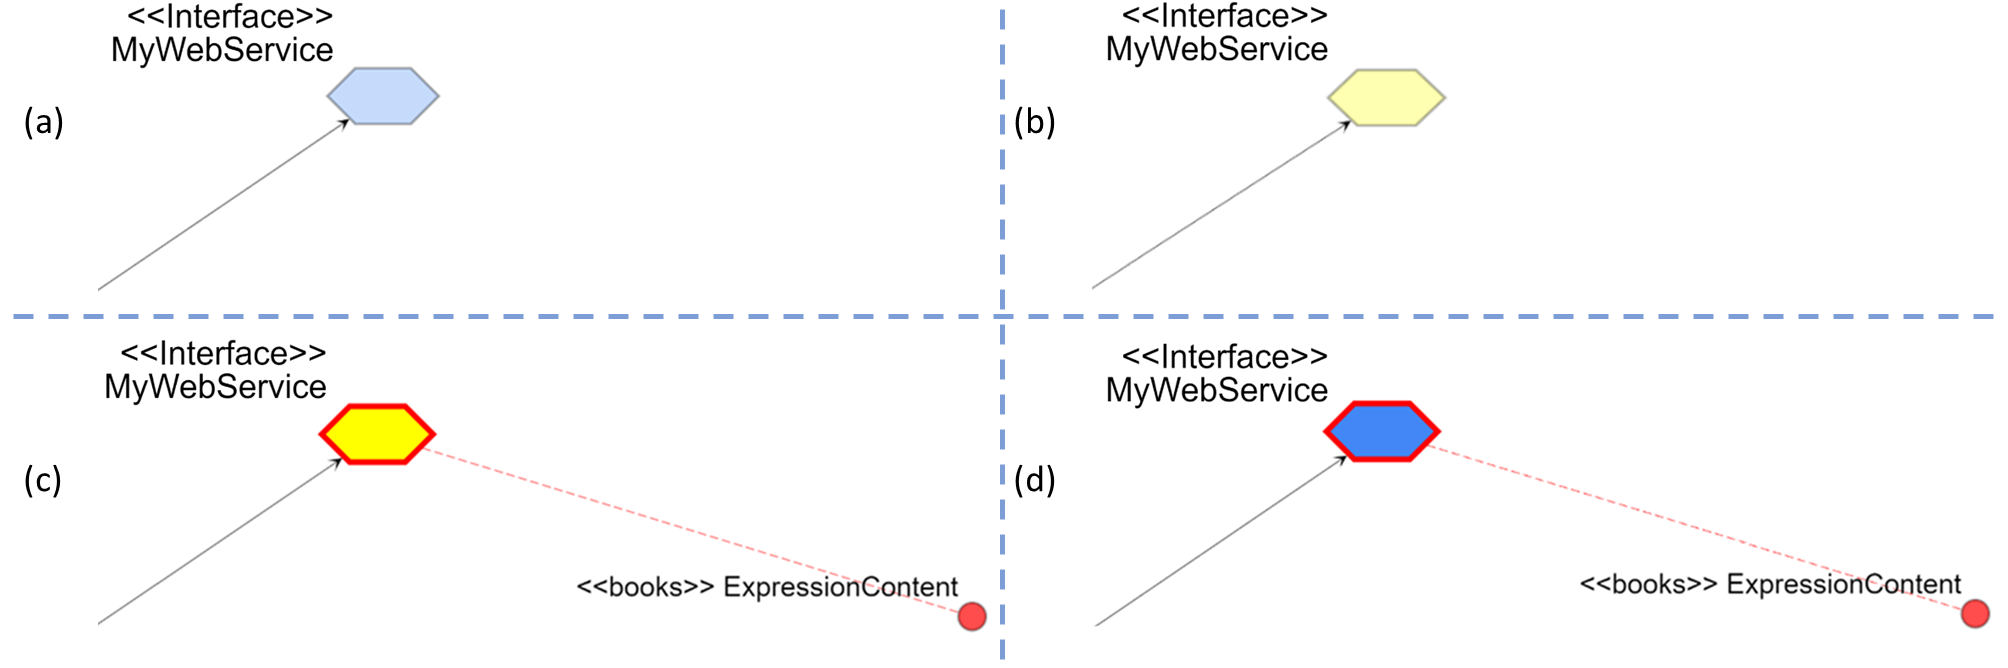
\includegraphics[scale=0.3]{4-grasews/imagens/grasews-anotacao-semantica-compartilhada-com-questoes.png}
    %}
    \centering
    \caption[Uso de questões para a anotação semântica de forma compartilhada]{\textbf{Uso de questões para a anotação semântica de forma compartilhada.} (a) Estado inicial da interface WSDL. (b) Interface WSDL com questão associada. (c) Interface WSDL com \textit{Model Reference} e com questão associada. (d) Interface WSDL com \textit{Model Reference}.}
    \label{fig:grasews-anotacao-semantica-compartilhada-com-questoes}
\end{figure}

Uma tarefa representa uma lista do trabalho necessário a ser realizado para concluir o processo de anotação semântica. A definição de uma ou mais tarefas pode contribuir para a coordenação do processo e anotação semântica entre múltiplos usuários envolvidos. Quando uma tarefa é concluída, esta tarefa pode ser marcada desta forma pelo usuário que a criou. Assim, os usuários mantém o controle das tarefas ainda pendentes de serem feitas.

Uma tarefa não é direcionada a um usuário específico, i.e., qualquer usuário envolvido na edição colaborativa é capaz de visualizar as tarefas para uma especificação WSDL. Além de visualizar a lista de tarefas, os usuários podem adicionar comentários, podendo contribuir para a finalização de uma tarefa. É possível ter múltiplos comentários de múltiplos usuários. A \figurename~\ref{fig:grasews-lista-tasks} ilustra a interface gráfica de Grasews para a listagem de tarefas. Por meio desta interface gráfica, um usuário pode adicionar comentários às tarefas e marcá-las como concluídas.

\begin{figure}[h]
    %\resizebox{\textwidth}{!}{
        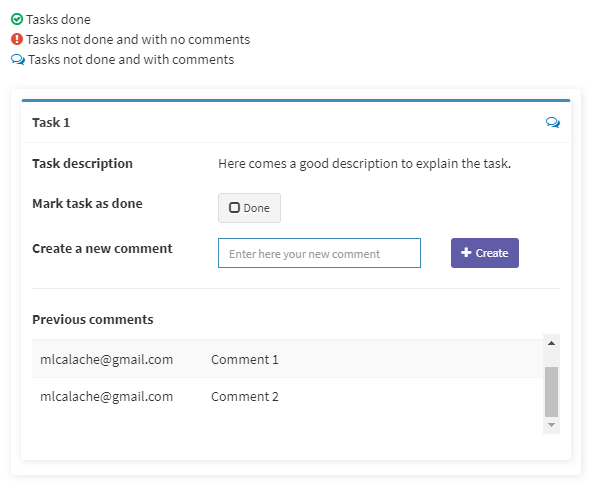
\includegraphics[scale=0.6]{4-grasews/imagens/grasews-lista-tasks.png}
    %}
    \centering
    \caption[Interface gráfica para a lista de tarefas]{\textbf{Interface gráfica para a lista de tarefas.}}
    \label{fig:grasews-lista-tasks}
\end{figure} % descomentar
\chapter{Prova de Conceito}\label{5-estudo-de-caso}

Este capítulo apresenta uma prova de conceito utilizando a ferramenta Grasews desenvolvida neste trabalho. Este capítulo tem por objetivo demonstrar o uso da ferramenta Grasews a fim de anotar semanticamente uma especificação WSDL por meio de notações visuais e de forma colaborativa.

Este capítulo está estruturado da seguinte forma: a seção \ref{5-estudo-de-caso-visao-geral} apresenta a metodologia utilizada para a condução da prova de conceito; a seção \ref{5-estudo-de-caso-processo-detalhado} apresenta os detalhes do processo realizado; e, finalmente, a seção \ref{5-estudo-de-caso-resultados} discute os resultados obtidos.
\section{Visão Geral}\label{5-estudo-de-caso-visao-geral}

A especificação WSDL, utilizada nesta prova de conceito, descreve um serviço web no domínio cinematográfico. A \figurename~\ref{fig:estudo-de-caso-grafo-wsdl} ilustra o grafo para a especificação WSDL utilizada nesta prova de conceito. A fim de simplificar o processo, a especificação WSDL contém apenas uma operação, cujo objetivo é a busca de filmes em um dado repositório. Este repositório e a implementação das operações em si não são relevantes para este trabalho. A operação de busca de filmes tem como resultado uma lista de filmes. Um filme é composto por uma lista de premiações (\texttt{Awards}), uma lista de atores (\texttt{Actor}), uma lista de produtoras (\texttt{Producer}), uma lista de diretores (\texttt{Director}), um país (\texttt{Country}), um gênero (\texttt{Genre}), um nome (\texttt{Name}) e um ano de lançamento (\texttt{Year}). Uma premiação (\texttt{Award}) é composta pelo nome (\texttt{Name}) e pelo ano da premiação (\texttt{Year}). Um ator (\texttt{Actor}) é composto pelo primeiro nome (\texttt{FirstName}) e pelo sobrenome (\texttt{LastName}). Uma produtora (\texttt{Producer}) é composta pelo nome (\texttt{Name}). Um diretor (\texttt{Director}) é composto pela data de nascimento (\texttt{DateOfBirth}), pelo primeiro nome (\texttt{FirstName}) e pelo sobenome (\texttt{LastName}). Um país (\texttt{Country}) é composto pelo nome (\texttt{Name}). Por fim, um gênero (\texttt{Genre}) é composto pelo nome (\texttt{Name}).

\begin{landscape}
    \begin{figure}[h]
        %\resizebox{\textwidth}{!}{
            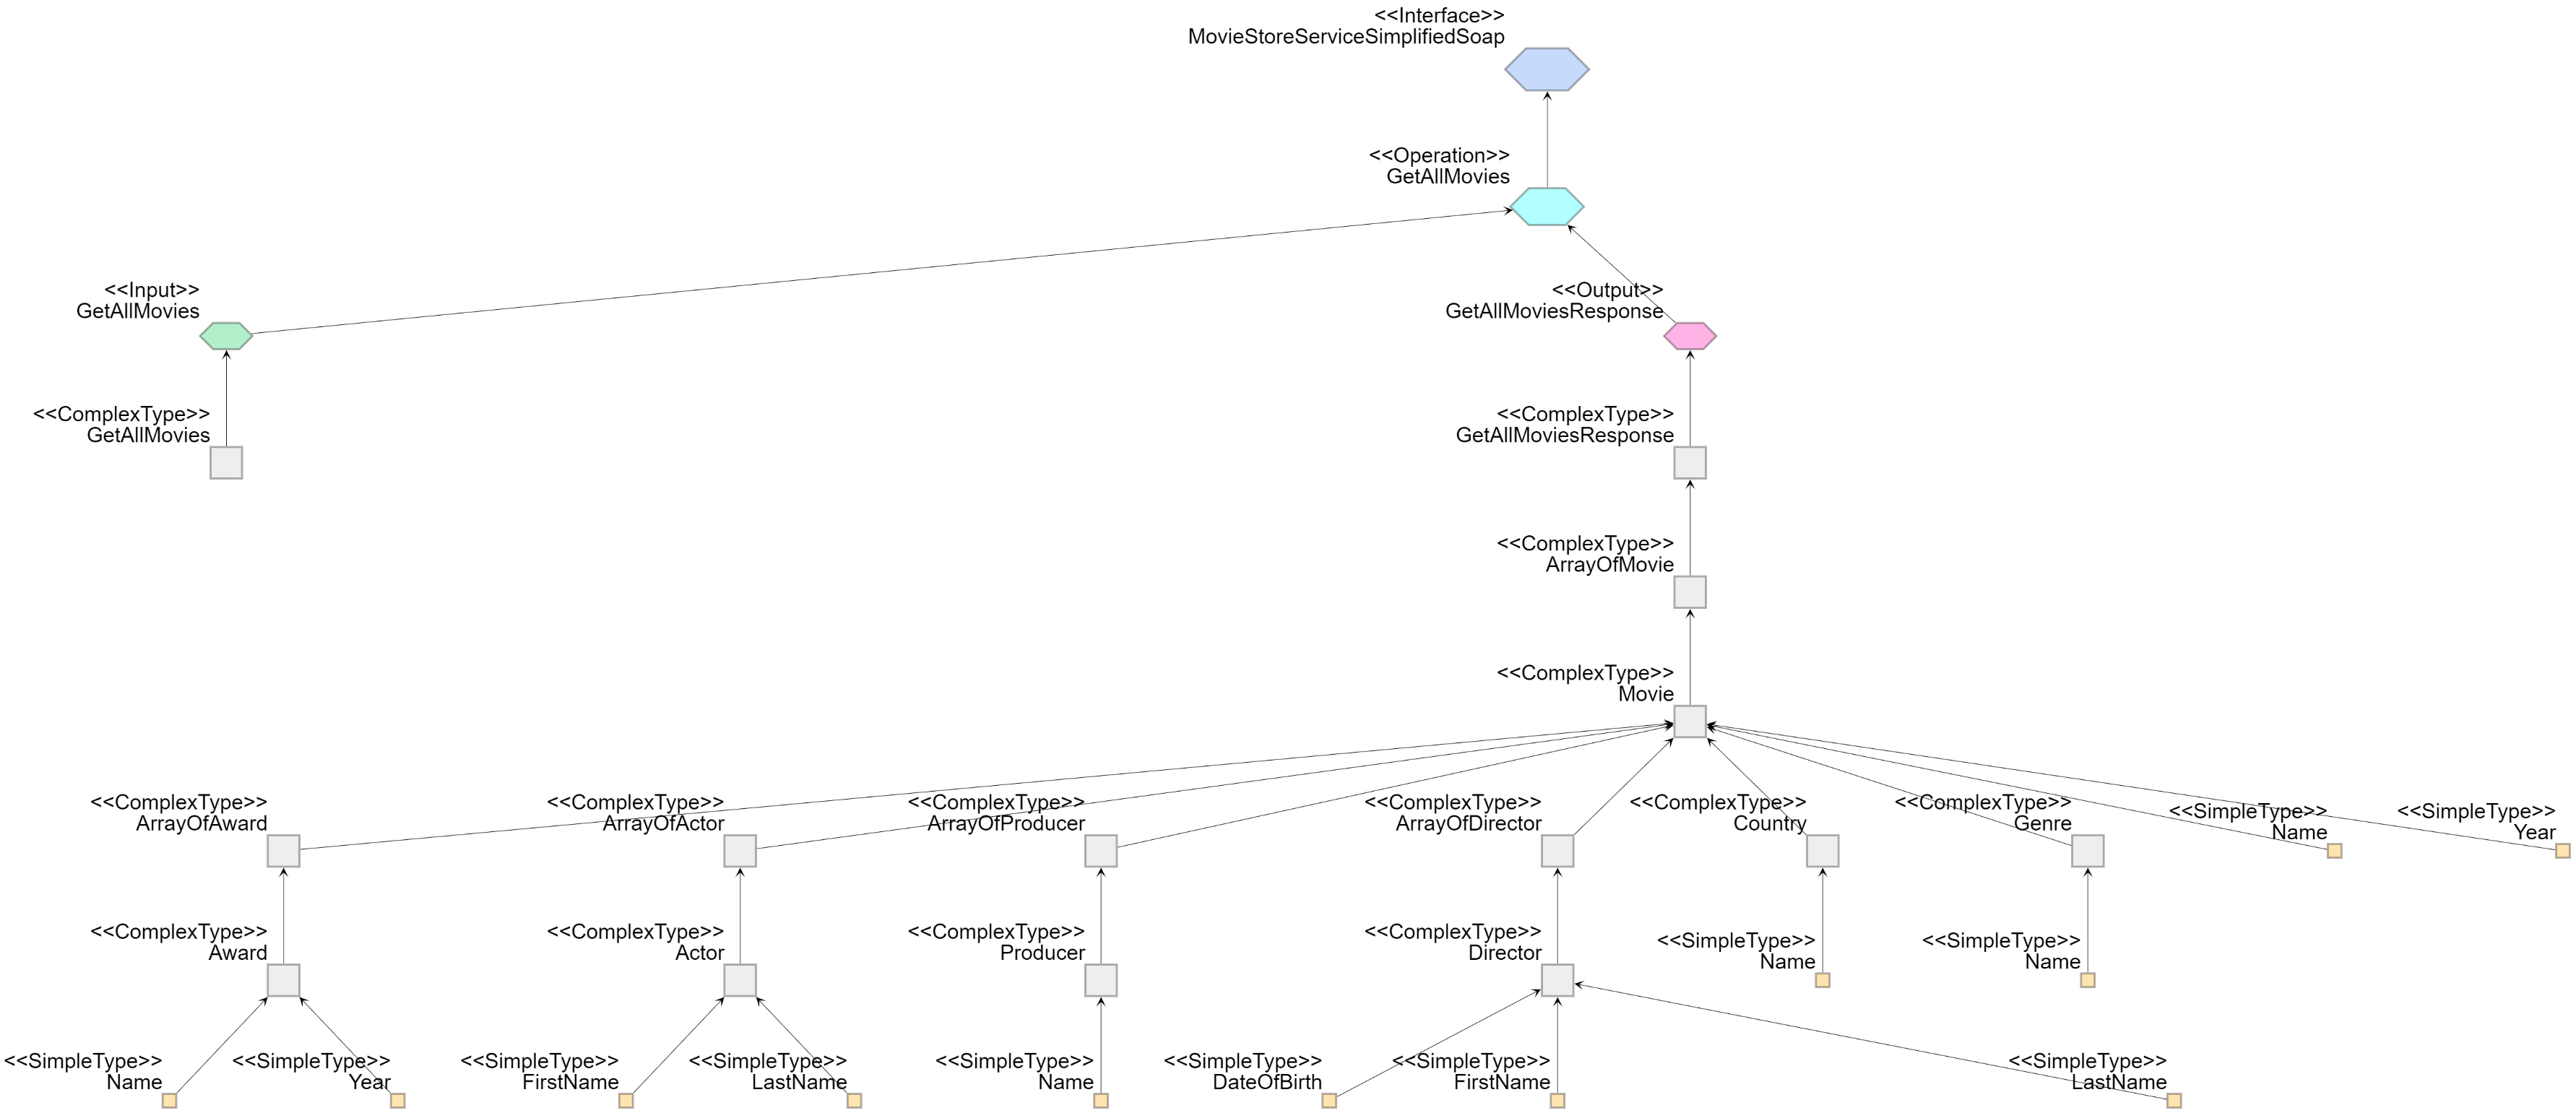
\includegraphics[scale=0.65]{5-grasews-estudo-de-caso/imagens/estudo-de-caso-grafo-wsdl.png}
        %}
        \centering
        \caption[Grafo da especificação WSDL utilizada na prova de conceito]{\textbf{Grafo da especificação WSDL utilizada na prova de conceito.}}
        \label{fig:estudo-de-caso-grafo-wsdl}
    \end{figure}
\end{landscape}

O documento de especificação WSDL deste processo possui o nome \break\texttt{MovieStoreServiceSimplified2.0} e encontra-se disponível no endereço \url{https://raw.githubusercontent.com/mlcalache/wsdls/master/MovieStoreServiceSimplified2.0.wsdl}. Adicionalmente, esta especificação WSDL está disponível no Anexo \ref{anexo-WSDL-estudo-de-caso}.

A fim de termos todos os artefatos necessários para apresentar este processo, em conjunto com a especificação WSDL, utilizamos a ontologia OWL \texttt{MovieOntology}~\cite{MOVIEONTOLOGY-2019}. A ontologia contém hierarquias de conceito para categorização de filmes que permitem a apresentação amigável de descrições de filmes. Esta ontologia foi desenvolvida pelo Departamento de Informática da Universidade de Zurique.

Neste processo, dois usuários trabalharam colaborativamente na anotação semântica da especificação WSDL. O primeiro usuário, denominado \texttt{Usuário A}, consiste de desenvolvedor de serviços web, enquanto que o segundo usuário, denominado \texttt{Usuário B}, consiste de um especialista no domínio cinematográfico. O \texttt{Usuário A} é possui o conhecimento especializado na tecnologia envolvida no desenvolvimento de serviços web semânticos e acerca de quais elementos WSDL/XSD devem ser anotados. Entretanto, o \texttt{Usuário A} não possui o conhecimento especializado no domínio e, consequentemente, acerca de quais termos da ontologia que devem ser utilizados na anotação. Eis que surge o importante papel do \texttt{Usuário B}, que auxiliou o \texttt{Usuário A} na solução de dúvidas e na finalização de tarefas para a anotação semântica da especificação WSDL.
\section{Detalhes do processo}\label{5-estudo-de-caso-processo-detalhado}

A seguir são listados os passos que compuseram o processo de anotação semântica de forma colaborativo apresentado por este estudo de caso.

\subsection{Passo 1 - Compartilhamento do Projeto}\label{estudo-de-caso-passo1-ambiente-de-trabalho-compartilhado}

O primeiro usuário, denominado \texttt{Usuário A}, já encontrava-se cadastrado na ferramenta e identificado pelo nome de usuário \texttt{mlcalache@gmail.com}. Este usuário foi responsável por carregar a especificação WSDL e a ontologia OWL na ferramenta. O \texttt{Usuário A} também foi responsável por compartilhar o projeto, i.e., a especificação WSDL e a ontologia OWL, com um segundo usuário por meio do \textit{e-mail} \texttt{usuariograsews@gmail.com}. Este segundo usuário, denominado \texttt{Usuário B}, ainda não estava cadastrado na ferramenta. O \texttt{Usuário B} recebeu um \textit{e-mail} com um convite para o trabalho colaborativo. A \figurename~\ref{fig:estudo-de-caso-compartilhar-com-email} ilustra a tela de Grasews informar o \textit{e-mail} do usuário com o qual ele deseja convidar para a edição colaborativa. Já a \figurename~\ref{fig:estudo-de-caso-email-convite} ilustra o \textit{e-mail} recebido pelo \texttt{Usuário B}.

%\begin{landscape}
    \begin{figure}[h]
        %\resizebox{\textwidth}{!}{
            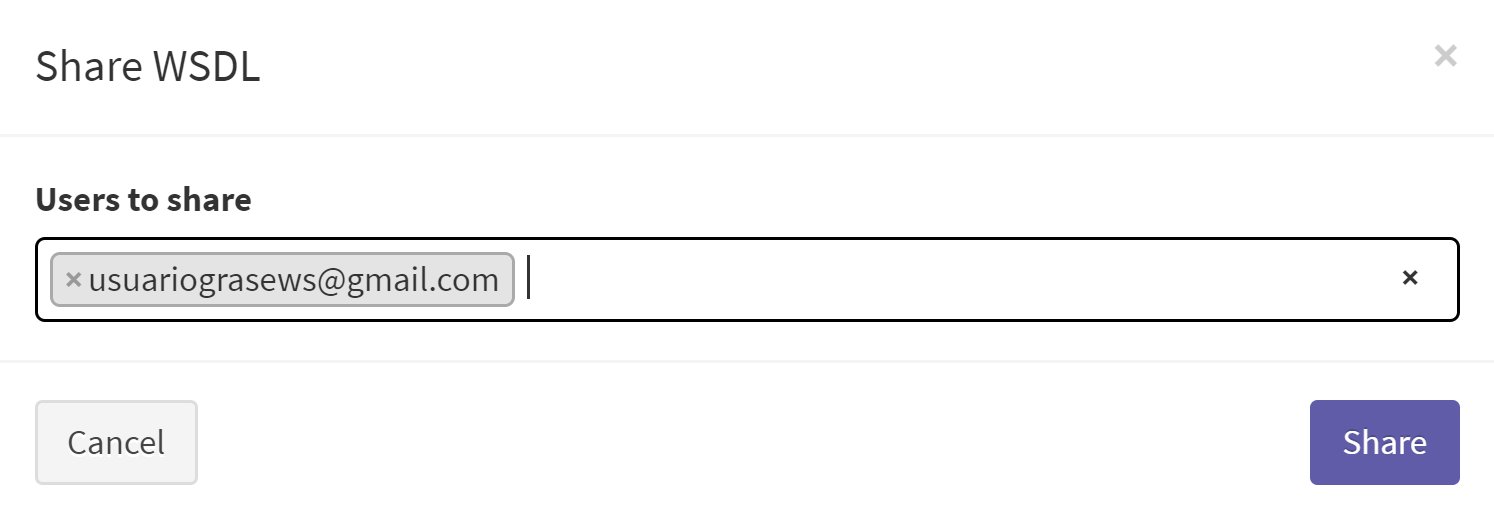
\includegraphics[scale=0.7]{5-grasews-estudo-de-caso/imagens/estudo-de-caso-compartilhar-com-email.png}
        %}
        \centering
        \caption[Compartilhamento do projeto com um outro usuário]{\textbf{Compartilhamento do projeto com um outro usuário.}}
        \label{fig:estudo-de-caso-compartilhar-com-email}
    \end{figure}
%\end{landscape}

%\begin{landscape}
    \begin{figure}[h]
        %\resizebox{\textwidth}{!}{
            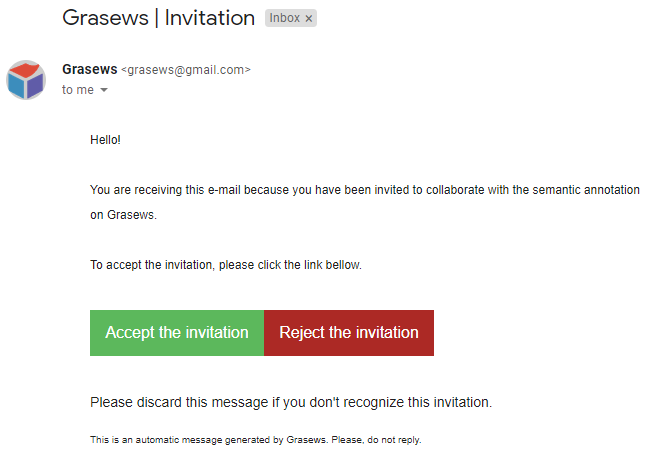
\includegraphics[scale=1.5]{5-grasews-estudo-de-caso/imagens/estudo-de-caso-email-convite.png}
        %}
        \centering
        \caption[\textit{E-mail} de convite para um usuário para o trabalho colaborativo]{\textbf{\textit{E-mail} de convite para um usuário para o trabalho colaborativo.}}
        \label{fig:estudo-de-caso-email-convite}
    \end{figure}
%\end{landscape}

O \texttt{Usuário B}, portanto, teve que se cadastrar na ferramenta. A \figurename~\ref{fig:estudo-de-caso-criar-novo-usuario-por-convite} ilustra a tela de cadastro de um novo usuário por meio de um convite de colaboração.

%\begin{landscape}
    \begin{figure}[h]
        %\resizebox{\textwidth}{!}{
            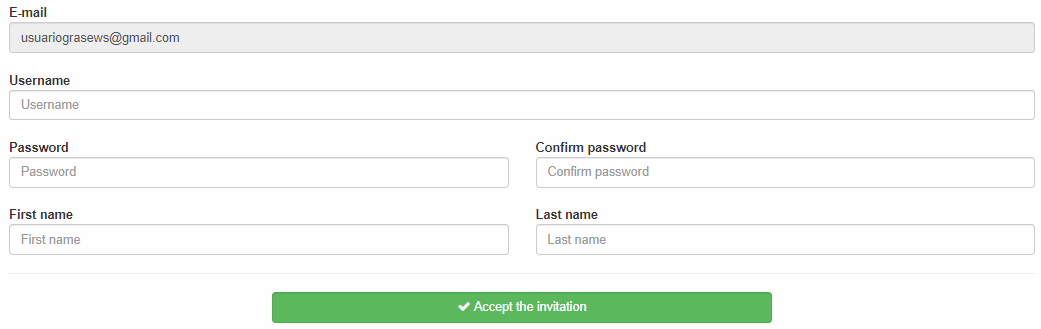
\includegraphics[scale=1.5]{5-grasews-estudo-de-caso/imagens/estudo-de-caso-criar-novo-usuario-por-convite.png}
        %}
        \centering
        \caption[Tela de cadastro de um novo usuário por meio de um convite de colaboração]{\textbf{Tela de cadastro de um novo usuário por meio de um convite de colaboração.}}
        \label{fig:estudo-de-caso-criar-novo-usuario-por-convite}
    \end{figure}
%\end{landscape}

Após ter-se cadastrado e autenticado na ferramenta, o \texttt{Usuário B} pode abrir a mesma especificação WSDL compartilhada pelo \texttt{Usuário A}. A \figurename~\ref{fig:estudo-de-caso-wsdl-compartilhado-disponivel-para-usuario} ilustra a especificação \texttt{MovieStoreServiceSimplified2.0} disponível para o \texttt{Usuário B}.

%\begin{landscape}
    \begin{figure}[h]
        %\resizebox{\textwidth}{!}{
            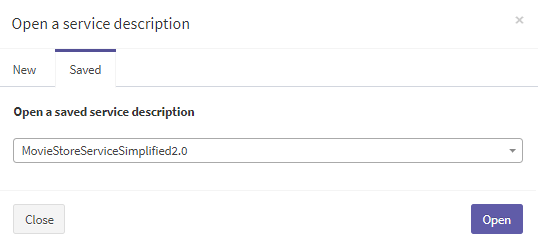
\includegraphics[scale=1.5]{5-grasews-estudo-de-caso/imagens/estudo-de-caso-wsdl-compartilhado-disponivel-para-usuario.png}
        %}
        \centering
        \caption[Especificação WSDL disponível para o \texttt{Usuário B}]{\textbf{Especificação WSDL disponível para o \texttt{Usuário B}.}}
        \label{fig:estudo-de-caso-wsdl-compartilhado-disponivel-para-usuario}
    \end{figure}
%\end{landscape}

\subsection{Passo 2 - Questões}\label{estudo-de-caso-passo2-questoes}

Após os dois usuários terem acesso à mesma especificação WSDL de forma compartilhada, um conjunto de questões relacionadas a elementos da especificação WSDL foram criadas pelos dois usuários.

%A \figurename~\ref{fig:estudo-de-caso-criar-questao} ilustra a tela de Grasews durante a criação de uma questão pelo \texttt{Usuário A}. Neste exemplo, o \texttt{Usuário A} criou uma questão para o elemento tipo complexo XSD \texttt{Genre}. O título de sua questão foi \textit{"Genre meaning"} e a questão em si foi \textit{"What genre stands for?"}.

%%\begin{landscape}
%    \begin{figure}[h]
%        %\resizebox{\textwidth}{!}{
%            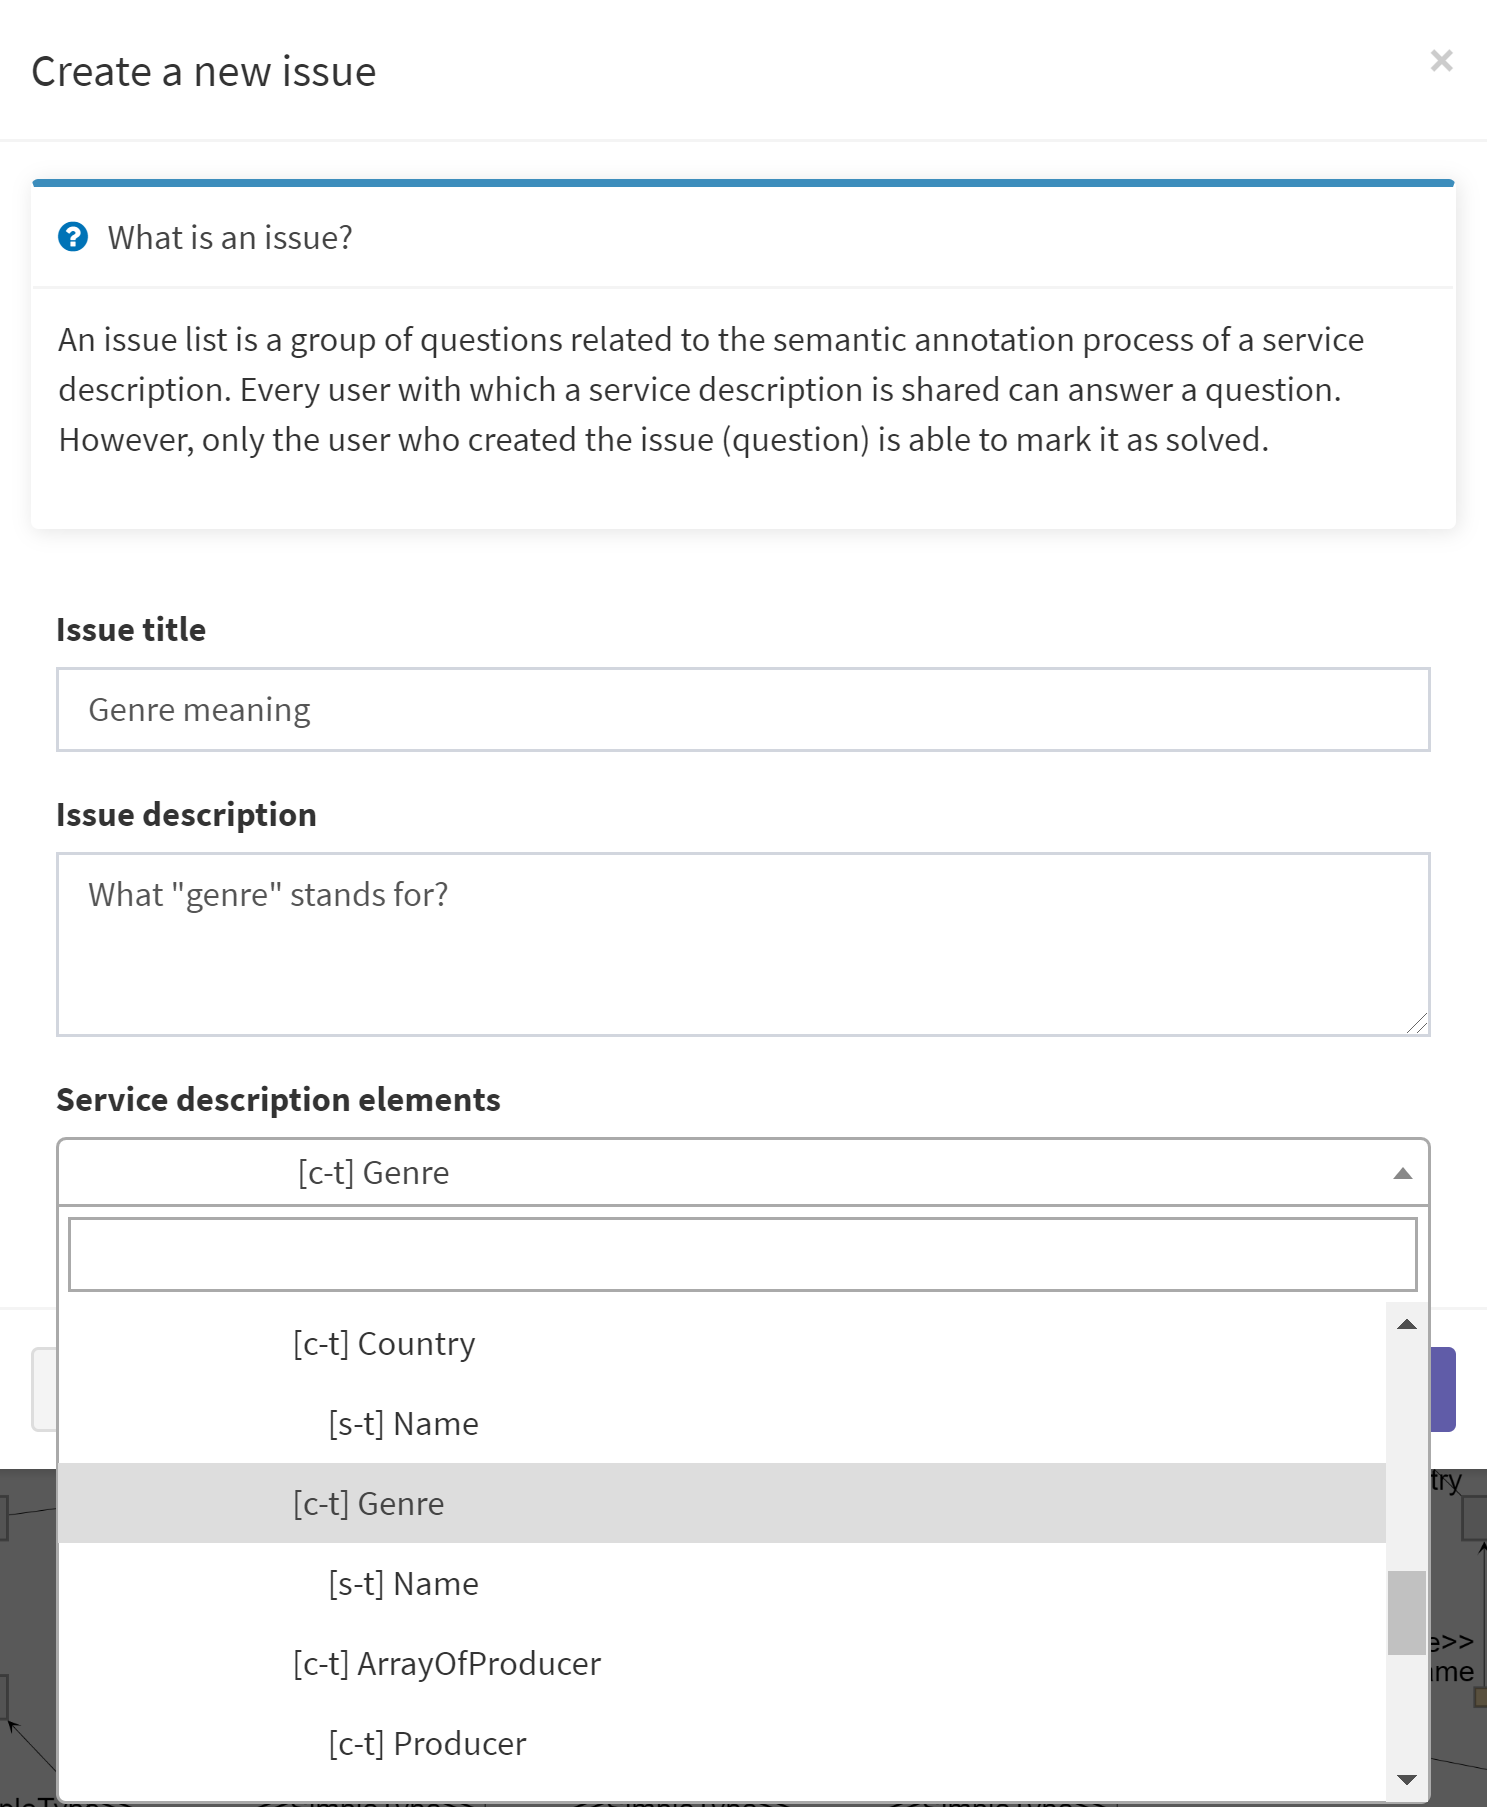
\includegraphics[scale=0.6]{5-grasews-estudo-de-caso/imagens/estudo-de-caso-criar-questao.png}
%        %}
%        \centering
%        \caption[Tela de criação de uma questão pelo \texttt{Usuário A}]{\textbf{Tela de criação de uma questão pelo \texttt{Usuário A}.}}
%        \label{fig:estudo-de-caso-criar-questao}
%    \end{figure}
%%\end{landscape}

Logo que uma nova questão era criada por um usuário, o outro usuário recebia notificações acerca da nova questão. Adicionalmente, o grafo foi automaticamente atualizado a cada questão criada, contendo, portanto, a representação visual para os elementos WSDL/XSD com questões questões associadas. A \figurename~\ref{fig:estudo-de-caso-grafo-wsdl-com-questao} ilustra o elemento tipo complexo XSD \texttt{Genre} com a notação visual para um elemento WSDL/XSD com uma questão, disponível para ambos os usuários. 

%\begin{landscape}
    \begin{figure}[h]
        %\resizebox{\textwidth}{!}{
            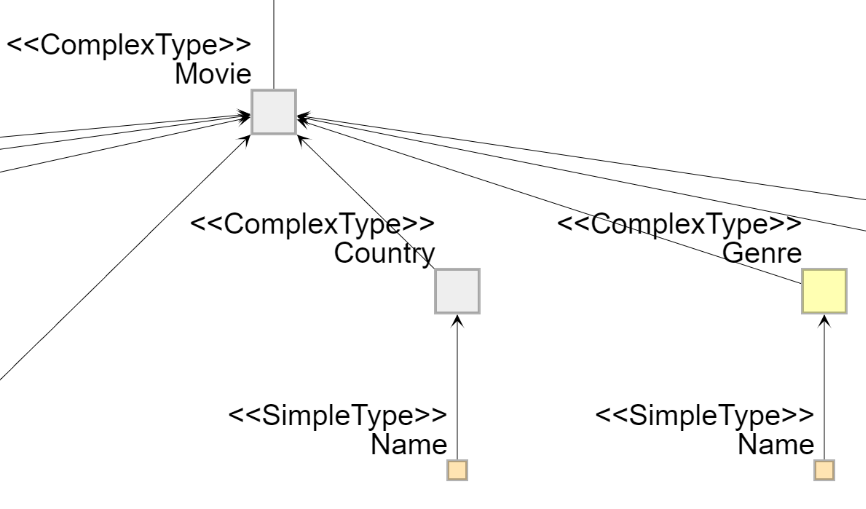
\includegraphics[scale=1]{5-grasews-estudo-de-caso/imagens/estudo-de-caso-grafo-wsdl-com-questao.png}
        %}
        \centering
        \caption[Notação visual para o elemento tipo complexo XSD \texttt{Genre} com uma questão]{\textbf{Notação visual para o elemento tipo complexo XSD \texttt{Genre} com uma questão.}}
        \label{fig:estudo-de-caso-grafo-wsdl-com-questao}
    \end{figure}
%\end{landscape}

De forma assíncrona à criação das questões, ambos usuários adicionaram respostas a elas. O \texttt{Usuário A} adicionou pelo menos uma resposta para cada questão criada pelo \texttt{Usuário A}, enquanto que o \texttt{Usuário B} adicionou pelo menos uma resposta para cada questão criada pelo \texttt{Usuário A}.

Ao passo que as anotações foram feitas e validadas com o auxílio da lista de questões, estas foram marcadas como resolvidas. Ao fim do processo, todas as questões foram marcadas como resolvidas. A seguir são listadas as questões criadas durante o processo.

\begin{tcolorbox}
    \begin{enumerate}[label=(Q\arabic*)]
    %\begin{enumerate}[label={\arabic*}]
        
        % Configura um espaço maior entre parágrafos das questões
        \setlength{\parskip}{0.55cm}
    
		%%%%%%%%%%%%%%%%%%%%%%%%%%%%%%%%%%%%%%%%%%%%%%%%
		
        \item 
        \textbf{Título}: Array of Awards?
        \\
        \textbf{Questão}: Does it mean it is possible to have multiple awards for a single movie?
        \\
        \textbf{Elemento WSDL/XSD}: [c-t] ArrayOfAward
        \\
        \textbf{Usuário}: mlcalache@gmail.com
        \\
        \textbf{Respostas}:
        \begin{enumerate}
            \item
                \textbf{Usuário}: \textit{usuariograsews@gmail.com}
                \\
                \textbf{Resposta}: \textit{Yes. A movie can have multiple awards, such as Oscar and Golden Globe awards.}
        \end{enumerate}
        
        %%%%%%%%%%%%%%%%%%%%%%%%%%%%%%%%%%%%%%%%%%%%%%%%
        
        \item 
        \textbf{Título}: Genre meaning?
        \\
        \textbf{Questão}: What genre stands for?
        \\
        \textbf{Elemento WSDL/XSD}: [c-t] Genre
        \\
        \textbf{Usuário}: mlcalache@gmail.com
        \\
        \textbf{Respostas}:
        \begin{enumerate}
            \item
                \textbf{Usuário}: \textit{usuariograsews@gmail.com}
                \\
                \textbf{Resposta}: \textit{This is the movie category, such as Drama, Comedy, SciFi, etc.}
        \end{enumerate}

        %%%%%%%%%%%%%%%%%%%%%%%%%%%%%%%%%%%%%%%%%%%%%%%%
        
        \item 
        \textbf{Título}: Annotate the complex type of the simple type?
        \\
        \textbf{Questão}: Shoud I annotate the country complex type or the country name simple type?
        \\
        \textbf{Elemento WSDL/XSD}: [c-t] Country
        \\
        \textbf{Usuário}: usuariograsews@gmail.com
        \\
        \textbf{Respostas}:
        \begin{enumerate}
            \item
                \textbf{Usuário}: \textit{mlcalache@gmail.com}
                \\
                \textbf{Resposta}: \textit{Let's focus on the complex types.}
        \end{enumerate}
        
		%%%%%%%%%%%%%%%%%%%%%%%%%%%%%%%%%%%%%%%%%%%%%%%%
        
    % Reconfigura o espaço entre parágrafos
    \setlength{\parskip}{0.2cm}
        
    \end{enumerate}
\end{tcolorbox}

\begin{tcolorbox}
    
    \begin{enumerate}[label=(Q\arabic*)]
        
        % Configura um espaço maior entre parágrafos das questões
        \setlength{\parskip}{0.55cm}
        
        \setcounter{enumi}{3}
        
        %%%%%%%%%%%%%%%%%%%%%%%%%%%%%%%%%%%%%%%%%%%%%%%%
        
        \item 
        \textbf{Título}: Year of movie?
        \\
        \textbf{Questão}: Is there any problem if we don’t have an ontology term for the year of the movie? And what about other elements which we also don’t have an ontology term?
        \\
        \textbf{Elemento WSDL/XSD}: [s-t] Year
        \\
        \textbf{Usuário}: usuariograsews@gmail.com
        \\
        \textbf{Respostas}:
        \begin{enumerate}
            \item
                \textbf{Usuário}: \textit{mlcalache@gmail.com}
                \\
                \textbf{Resposta}: \textit{Let's skip the simple types for now. Let's focus on the complex types. I've created a list of tasks, which does not contemplate the simple types.}
        \end{enumerate}
        
        %%%%%%%%%%%%%%%%%%%%%%%%%%%%%%%%%%%%%%%%%%%%%%%%
        
        \item 
        \textbf{Título}: Actor name?
        \\
        \textbf{Questão}: Since we don’t have a distinct ontology term for the first name and the last name, I suggest we annotate only the Actor element and leave the first and the last name with no annotation. What do you think?
        \\
        \textbf{Elemento WSDL/XSD}: [s-t] FirstName
        \\
        \textbf{Usuário}: usuariograsews@gmail.com
        \\
        \textbf{Respostas}:
        \begin{enumerate}
            \item
                \textbf{Usuário}: \textit{mlcalache@gmail.com}
                \\
                \textbf{Resposta}: \textit{Let's skip the simple types for now. Let's focus on the complex types. I've created a list of tasks, which does not contemplate the simple types.}
        \end{enumerate}
        
		%%%%%%%%%%%%%%%%%%%%%%%%%%%%%%%%%%%%%%%%%%%%%%%%
        
    % Reconfigura o espaço entre parágrafos
    \setlength{\parskip}{0.2cm}
        
    \end{enumerate}
\end{tcolorbox}

%A \figurename~\ref{fig:estudo-de-caso-lista-questoes-nao-resolvidas} ilustra a lista de questões criadas pelos usuários. Note que, pelo ícone e a cor vermelha, não há respostas ainda adicionadas às questões e as questões ainda não estão marcadas como resolvidas.

%%\begin{landscape}
%    \begin{figure}[h]
%        %\resizebox{\textwidth}{!}{
%            \includegraphics[scale=0.8]{5-grasews-estudo-de-caso/imagens/estudo-de-caso-lista-questoes-nao-resol%vidas.png}
%        %}
%        \centering
%        \caption[Lista de questões criadas para a prova de conceito na ferramenta Grasews]{\textbf{Lista de %questões criadas para a prova de conceito na ferramenta Grasews.}}
%        \label{fig:estudo-de-caso-lista-questoes-nao-resolvidas}
%    \end{figure}
%%\end{landscape}

\subsection{Passo 3 - Tarefas}\label{estudo-de-caso-passo3-tarefas}

Simultaneamente com a criação e a resolução das questões, o \texttt{Usuário A} criou uma lista de tarefas que foi compartilhada com o \texttt{Usuário B}. Devido à utilização de conceitos de fácil entendimento do domínio cinematográfico, algumas anotações semânticas podem ser consideradas bastante simples. Neste sentido, o \texttt{Usuário A} foi capaz de realizar anotações semânticas, seguindo a lista de tarefas. O \texttt{Usuário B} contribuiu efetivamente no processo tanto para as iniciadas pelo \texttt{Usuário A}, onde \texttt{Usuário B} pode revisar e corrigir, quanto para as tarefas pendentes, onde \texttt{Usuário B} pode criar as anotações semânticas.

Ao passo que as anotações foram feitas e validadas com o auxílio de tarefas, estas foram marcadas como finalizadas. Ao fim do processo, todas as tarefas foram marcadas como finalizadas. A seguir, são listadas as tarefas criadas durante o processo. 

%Por fim, a \tablename~\ref{tab:estudo-de-caso-lista-questoes} lista as tarefas criadas durante o processo. \hl{fazer}

\begin{tcolorbox}
    \begin{enumerate}[label=(T\arabic*)]
    %\begin{enumerate}[label={\arabic*}]
        
        % Configura um espaço maior entre parágrafos das questões
        \setlength{\parskip}{0.55cm}
        
		%%%%%%%%%%%%%%%%%%%%%%%%%%%%%%%%%%%%%%%%%%%%%%%%
    
        \item 
        \textbf{Título}: Annotate Award Complex Type
        \\
        \textbf{Tarefa}: Annotate Award Complex Type with a Model Reference
        
		%%%%%%%%%%%%%%%%%%%%%%%%%%%%%%%%%%%%%%%%%%%%%%%%
    
        \item 
        \textbf{Título}: Annotate Actor Complex Type
        \\
        \textbf{Tarefa}: Annotate Actor Complex Type with a Model Reference
        
		%%%%%%%%%%%%%%%%%%%%%%%%%%%%%%%%%%%%%%%%%%%%%%%%
    
        \item 
        \textbf{Título}: Annotate Producer Complex Type
        \\
        \textbf{Tarefa}: Annotate Producer Complex Type with a Model Reference
        
		%%%%%%%%%%%%%%%%%%%%%%%%%%%%%%%%%%%%%%%%%%%%%%%%
        
%    % Reconfigura o espaço entre parágrafos
%    \setlength{\parskip}{0.2cm}
%    
%    \end{enumerate}
%\end{tcolorbox}
%
%\begin{tcolorbox}
%    \begin{enumerate}[label=(T\arabic*)]
%    %\begin{enumerate}[label={\arabic*}]
%        
%        % Configura um espaço maior entre parágrafos das questões
%        \setlength{\parskip}{0.55cm}
%        
%        \setcounter{enumi}{3}
        
		%%%%%%%%%%%%%%%%%%%%%%%%%%%%%%%%%%%%%%%%%%%%%%%%
    
        \item 
        \textbf{Título}: Annotate Director Complex Type
        \\
        \textbf{Tarefa}: Annotate Director Complex Type with a Model Reference
        
		%%%%%%%%%%%%%%%%%%%%%%%%%%%%%%%%%%%%%%%%%%%%%%%%
		
        \item 
        \textbf{Título}: Annotate Country Complex Type
        \\
        \textbf{Tarefa}: Annotate Country Complex Type with a Model Reference
        
		%%%%%%%%%%%%%%%%%%%%%%%%%%%%%%%%%%%%%%%%%%%%%%%%
		
        \item 
        \textbf{Título}: Annotate Genre Complex Type
        \\
        \textbf{Tarefa}: Annotate Genre Complex Type with a Model Reference
        
		%%%%%%%%%%%%%%%%%%%%%%%%%%%%%%%%%%%%%%%%%%%%%%%%
		
        \item 
        \textbf{Título}: Annotate Movie Complex Type
        \\
        \textbf{Tarefa}: Annotate Movie Complex Type with a Model Reference
        
		%%%%%%%%%%%%%%%%%%%%%%%%%%%%%%%%%%%%%%%%%%%%%%%%
        
    % Reconfigura o espaço entre parágrafos
    \setlength{\parskip}{0.2cm}
    
    \end{enumerate}
\end{tcolorbox}

%A \figurename~\ref{fig:estudo-de-caso-lista-tarefas} ilustra a interface gráfica de Grasews para a lista de tarefas criadas pelo \texttt{Usuário A}.

%Note que, pelo ícone e a cor vermelha, não há comentários ainda adicionados às tarefas e as tarefas ainda não estão marcadas como finalizadas.

%%\begin{landscape}
%    \begin{figure}[h]
%        %\resizebox{\textwidth}{!}{
%            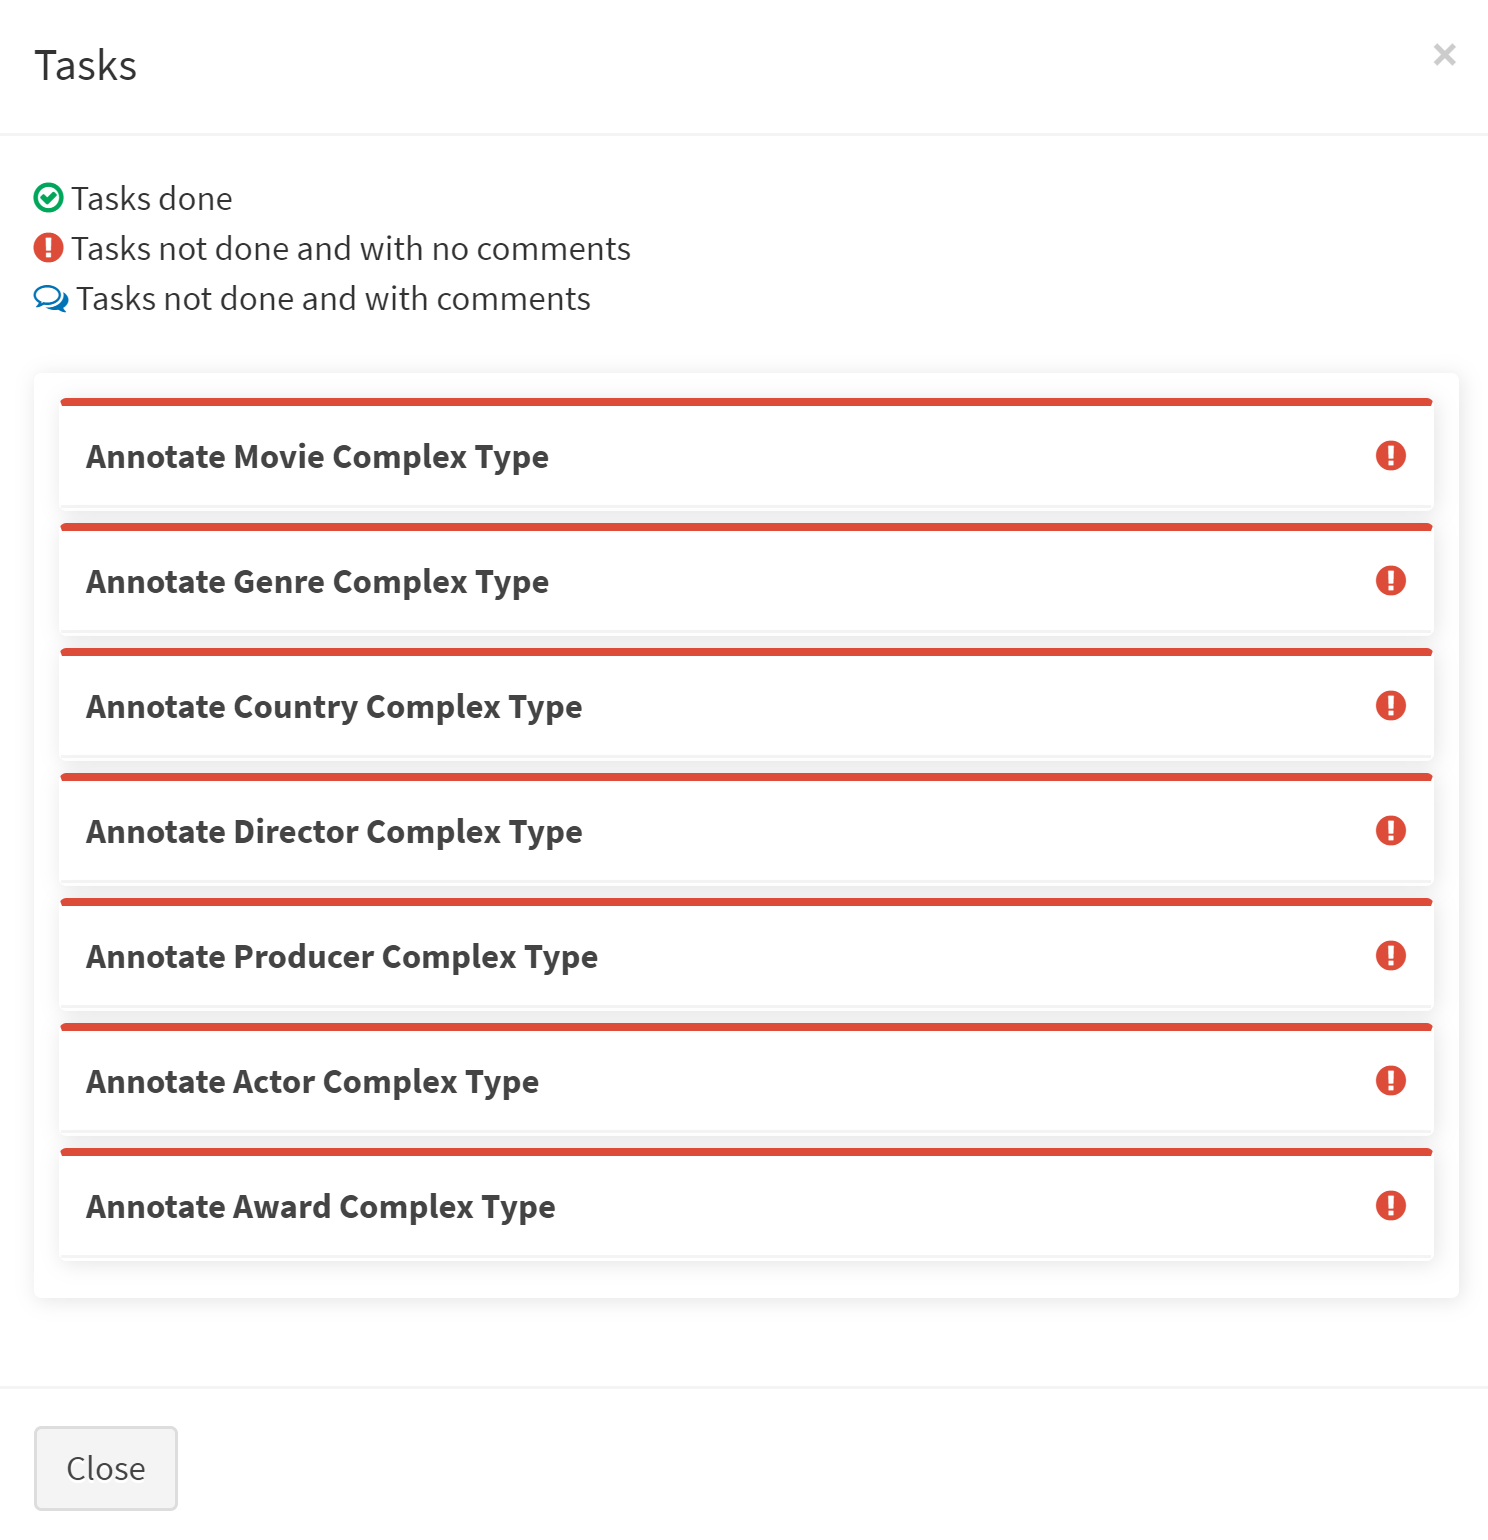
\includegraphics[scale=0.8]{5-grasews-estudo-de-caso/imagens/estudo-de-caso-lista-tarefas.png}
%        %}
%        \centering
%        \caption[Lista de tarefas criadas para a prova de conceito na ferramenta Grasews]{\textbf{Lista de %tarefas criadas para a prova de conceito na ferramenta Grasews.}}
%        \label{fig:estudo-de-caso-lista-tarefas}
%    \end{figure}
%%\end{landscape}

\iffalse
\begin{landscape}
    \begin{table}[ht!]
        \setlength{\tabcolsep}{10pt} % Default value: 6pt
        \renewcommand{\arraystretch}{1.5} % Default value: 1
        \centering
    	\caption[Lista de questões criadas durante o processo.]{\textbf{Lista de questões criadas durante o processo.}}
    	\label{tab:estudo-de-caso-lista-questoes}
    	%\resizebox{\textwidth}{!}{
    		\begin{tabular}{| >{\columncolor{Gray}}c | c | c | c | c | }
    			\hline
                \rowcolor{Gray}
    			
    			{\textbf{\#}} & \textbf{Título} & \textbf{Questão} & \textbf{Elemento WSDL/XSD} & \textbf{Usuário}
    			
    			%%%%%%%%%%%%%%%%%%%%%%%%%%%%%%%%%%%%%%%%%%%%%%%%
    			\\
    			\hline
    			{}
    			& {}
    			& {Does it mean it is}
    			& {}
    			& {}
    			\\
    			{}
    			& {}
    			& {possible to have multiple}
    			& {}
    			& {}
    			\\
    			\multirow{-2.5}{*}[3px]{1}
    			& \multirow{-2.5}{*}[3px]{Array Of Awards?}
    			& {awards for a single movie?}
    			& \multirow{-2.5}{*}[3px]{[c-t] ArrayOfAward}
    			& \multirow{-2.5}{*}[3px]{mlcalache@gmail.com}
    			
    			%%%%%%%%%%%%%%%%%%%%%%%%%%%%%%%%%%%%%%%%%%%%%%%%
    			
    			\\
                \hline
    			{2} & {Genre meaning?} & {What genre stands for?} & {[c-t] Genre} & {mlcalache@gmail.com}
    			
    			%%%%%%%%%%%%%%%%%%%%%%%%%%%%%%%%%%%%%%%%%%%%%%%%
    			
    			\\
    			\hline
    			{}
    			& {Annotate}
    			& {Shoud I annotate the}
    			& {}
    			& {}
    			\\
    			{}
    			& {complex type}
    			& {country complex type or}
    			& {}
    			& {}
    			\\
    			\multirow{-2.5}{*}[3px]{3}
    			& {or simple type?}
    			& {the country name simple type?}
    			& \multirow{-2.5}{*}[3px]{[c-t] Country}
    			& \multirow{-2.5}{*}[3px]{usuariograsews@gmail.com}
    			
    			%%%%%%%%%%%%%%%%%%%%%%%%%%%%%%%%%%%%%%%%%%%%%%%%
    			
    			\\
    			\hline
    			{}
    			& {}
    			& {Is there any problem if wedon't have}
    			& {}
    			& {}
    			\\
    			{}
    			& {}
    			& {an ontology term for the year}
    			& {}
    			& {}
    			\\
    			{}
    			& {}
    			& {of the movie? And what about}
    			& {}
    			& {}
    			\\
    			{}
    			& {}
    			& {other elements which we also}
    			& {}
    			& {}
    			\\
    			\multirow{-4.5}{*}[3px]{4}
    			& \multirow{-4.5}{*}[3px]{Year of movie?}
    			& {don't have an ontology term?}
    			& \multirow{-4.5}{*}[3px]{[s-t] Year}
    			& \multirow{-4.5}{*}[3px]{usuariograsews@gmail.com}
    			
    			%%%%%%%%%%%%%%%%%%%%%%%%%%%%%%%%%%%%%%%%%%%%%%%%
    			
    			\\
    			\hline
    			{}
    			& {}
    			& {Since we don't have a distinct ontology}
    			& {}
    			& {}
    			\\
    			{}
    			& {}
    			& {term for the first name and the last name,}
    			& {}
    			& {}
    			\\
    			{}
    			& {}
    			& {I suggest we annotate only the Actor element}
    			& {}
    			& {}
    			\\
    			{}
    			& {}
    			& {and leave the first and the last name}
    			& {}
    			& {}
    			\\
    			\multirow{-4.5}{*}[3px]{5}
    			& \multirow{-4.5}{*}[3px]{Actor name?}
    			& {with no annotation. What do you think?}
    			& \multirow{-4.5}{*}[3px]{[s-t] FirstName}
    			& \multirow{-4.5}{*}[3px]{usuariograsews@gmail.com}
    			
    			%%%%%%%%%%%%%%%%%%%%%%%%%%%%%%%%%%%%%%%%%%%%%%%%
    			
    			\\
                \hline
    		\end{tabular}
    	%}
    \end{table}
\end{landscape}
\fi

\iffalse
\begin{table}[ht!]
    \setlength{\tabcolsep}{10pt} % Default value: 6pt
    \renewcommand{\arraystretch}{1.5} % Default value: 1
    \centering
	\caption[Lista de tarefas criadas durante o processo.]{\textbf{Lista de tarefas criadas durante o processo.}}
	\label{tab:estudo-de-caso-lista-questoes}
	%\resizebox{\textwidth}{!}{
		\begin{tabular}{| >{\columncolor{Gray}}c | c | c | }
			\hline
            \rowcolor{Gray}
			{\#} & \textbf{Tarefa}
			\\
			\hline
			{1} & {bla bla bla}
			\\
            \hline
			{2} & {bla bla bla}
			\\ 
            \hline
			{3} & {bla bla bla}
			\\
            \hline
		\end{tabular}
	%}
\end{table}
\fi

\subsection{Passo 4 - Anotação Semântica}\label{estudo-de-caso-passo4-anotacao-semantica}

O último passo da prova de conceito consiste da anotação semântica da especificação WSDL.
Ambos usuários trabalharam simultaneamente na anotação semântica conforme a lista de tarefas criada pelo \texttt{Usuário A}. A anotação semântica foi feita tanto por meio do menu de contexto do grafo, quanto por meio do menu de contexto do menu \textit{tree-view} WSDL e do menu \textit{tree-view} OWL. 

O documento de especificação WSDL anotado encontra-se disponível no endereço \url{https://raw.githubusercontent.com/mlcalache/wsdls/master/MovieStoreServiceSimplified2.0-anotado.wsdl}. Adicionalmente, a especificação WSDL anotada está disponível no Anexo \ref{anexo-WSDL-anotado-estudo-de-caso}. Por fim, a \figurename~\ref{fig:estudo-de-caso-grafo-wsdl-anotado} ilustra o grafo WSDL do \texttt{Usuário B} após a conclusão das tarefas. Como resultado, temos a especificação WSDL anotada 

\begin{landscape}
    \begin{figure}[h]
        %\resizebox{\textwidth}{!}{
            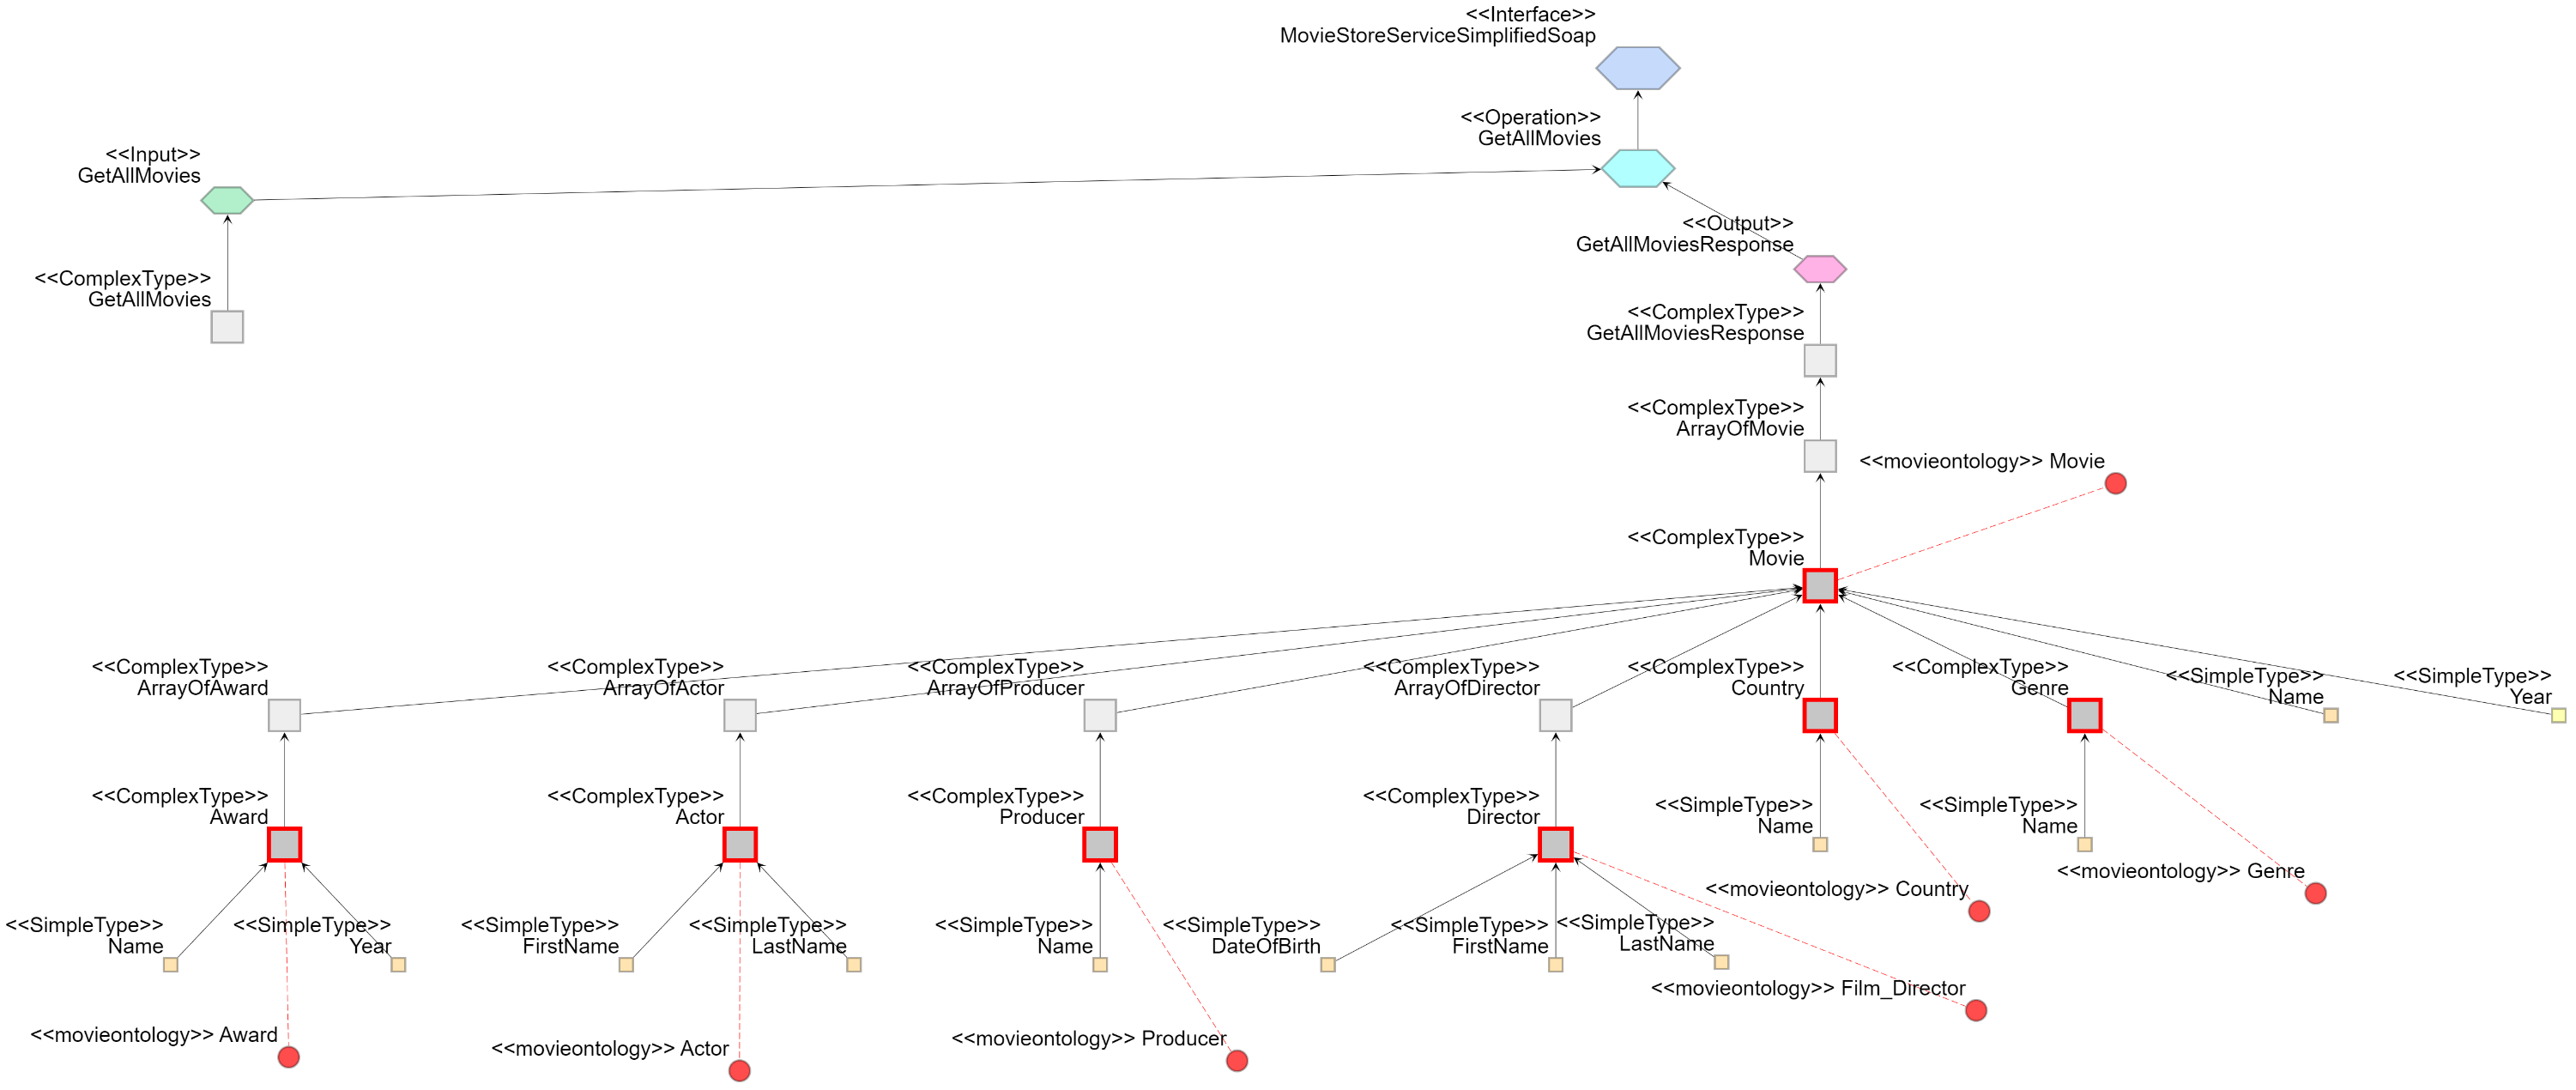
\includegraphics[scale=0.78]{5-grasews-estudo-de-caso/imagens/estudo-de-caso-grafo-wsdl-anotado.png}
        %}
        \centering
        \caption[Grafo da especificação WSDL anotada na prova de conceito]{\textbf{Grafo da especificação WSDL anotada na prova de conceito.}}
        \label{fig:estudo-de-caso-grafo-wsdl-anotado}
    \end{figure}
\end{landscape}
\section{Resultados}\label{5-estudo-de-caso-resultados}

Neste capítulo demonstramos o uso da ferramenta Grasews para a anotação semântica de uma especificação WSDL. O processo foi inteiramente conduzido por meio das notações visuais providas por Grasews juntamente com a edição colaborativa, envolvendo um desenvolvedor de serviços web e um especialista de domínio.

A utilização da ferramenta facilitou a anotação semântica da especificação WSDL utilizada nesta prova de conceito. Como a especificação WSDL foi criada para o propósito deste estudo de caso, não pudemos comparar os resultados obtidos com outro cenário, onde a especificação já estivesse anotada. O foco desta prova de conceito não foi validar os conceitos ontológicos utilizados na anotação semântica, mas sim validar o processo de anotação semântica auxiliado por notações visuais e pelo trabalho colaborativo por meio da ferramenta Grasews.

Nenhum URI de transformação para os atributos \textit{Lifting Schema Mapping} e \textit{Lowering Schema Mapping} foi utilizado durante o processo de prova de conceito.

A \tablename~\ref{tab:estudo-de-caso-elementos-wsdl-anotados} lista os elementos WSDL/XSD anotados durante a prova de conceito juntamente com os URIs da ontologia \texttt{MovieOntology} utilizados no atributo \textit{Model Reference}. Note que a ontologia \texttt{MovieOntology} utiliza conceitos provindos da ontologia \texttt{dbpedia}.

\begin{table}[ht!]
    \setlength{\tabcolsep}{10pt} % Default value: 6pt
    \renewcommand{\arraystretch}{1.5} % Default value: 1
    \centering
	\caption[Elementos WSDL/XSD anotados durante a prova de conceito.]{\textbf{Elementos WSDL/XSD anotados durante a prova de conceito.}}
	\label{tab:estudo-de-caso-elementos-wsdl-anotados}
	%\resizebox{\textwidth}{!}{
		\begin{tabular}{| >{\columncolor{Gray}}c | >{\centering\arraybackslash} p{9cm} | }
			\hline
            \rowcolor{Gray}
			\textbf{Elemento WSLD/XSD} & \textbf{URI de \textit{Model Reference}}
			\\
			\hline
			{Movie} & {\url{http://www.movieontology.org/2009/11/09/Movie}}
			\\
            \hline
            {Director} & {\url{http://dbpedia.org/page/Film\_Director}}
			\\ 
            \hline
			{Country} & {\url{http://dbpedia.org/ontology/Country}}
			\\
			\hline
			{Producer} & {\url{http://www.movieontology.org/2009/10/01/movieontology.owl\#Producer}}
			\\
			\hline
			{Actor} & {\url{http://dbpedia.org/ontology/Actor}}
			\\
			\hline
			{Award} & {\url{http://www.movieontology.org/2009/10/01/movieontology.owl\#Award}}
			\\
            \hline
		\end{tabular}
	%}
\end{table} % descomentar
\chapter{Conclusão}\label{7-conclusao}

Este trabalho teve por objetivo a investigação do suporte ferramental para o desenvolvimento de serviços web semânticos, segundo a abordagem SAWSDL`\cite{W3C-2007-SAWSDL}, por meio de notações visuais e de forma colaborativa. Este capítulo apresenta as principais contribuições deste trabalho, além de discutir sobre o uso e adoção de serviços web semânticos pela comunidade e apresentar os trabalhos futuros provenientes deste trabalho.

O capítulo está estruturado da seguinte forma: a seção \ref{7-conclusao-principais-contribuicoes} apresenta as principais contribuições deste trabalho; a seção \ref{7-conclusao-discussao} discute a abordagem proposta para a anotação semântica de serviços web; e, por fim, a seção \ref{7-conclusao-trabalhos-futuros} apresenta os trabalhos futuros.
\section{Principais Contribuições}\label{7-conclusao-principais-contribuicoes}

\lipsum[1]
\section{Discussão}\label{7-conclusao-discussao}

\lipsum[1]
\section{Trabalhos Futuros}\label{7-conclusao-trabalhos-futuros}

\lipsum[1] % descomentar

% ----------------------------------------------------------
% ELEMENTOS PÓS-TEXTUAIS
% ----------------------------------------------------------
% Retire o comentário somente se o padrão exigir que daqui para a
% frente não haja número de páginas.
%\postextual
% ----------------------------------------------------------

% ------
\bibliography{8-referencias/arquitetura,8-referencias/ferramentas-sws,8-referencias/tecnologias,8-referencias/notacaovisual,8-referencias/servicosweb,8-referencias/sistemascolaborativos,8-referencias/sws,8-referencias/estudo-de-caso,8-referencias/semantica-openapi,8-referencias/semantica-wadl}
% ------

% ----------------------------------------------------------
% Glossário
% ----------------------------------------------------------
%
% Consulte o manual da classe abntex2 para orientações sobre o glossário.
%
%\glossary

% ----------------------------------------------------------
% Apêndices
% ----------------------------------------------------------

% ---
% Inicia os apêndices e anexos
% ---
%\begin{apendicesenv}

% Imprime uma página indicando o início dos apêndices
\partapendices

\chapter{Estrutura Analítica de Projetos}\label{apendice-eap}

A estrutura analítica de projetos (EAP) da ferramenta Grasews é apresentada em quatro (4) partes. A \figurename~\ref{fig:grasews-eap-usuario} ilustra os sub-pacotes de trabalho e atividades a fim de entregar o pacote de trabalho denominado \texttt{Usuário}. A \figurename~\ref{fig:grasews-eap-wsdl} ilustra os sub-pacotes de trabalho e atividades a fim de entregar o pacote de trabalho denominado \texttt{WSDL}. A \figurename~\ref{fig:grasews-eap-owl} ilustra os sub-pacotes de trabalho e atividades a fim de entregar o pacote de trabalho denominado \texttt{OWL}. Finalmente, a \figurename~\ref{fig:grasews-eap-colaboracao} ilustra os sub-pacotes de trabalho e atividades a fim de entregar o pacote de trabalho denominado \texttt{Colaboração}.

%\begin{landscape}
    \begin{figure}[h]
        %\resizebox{\textwidth}{!}{
            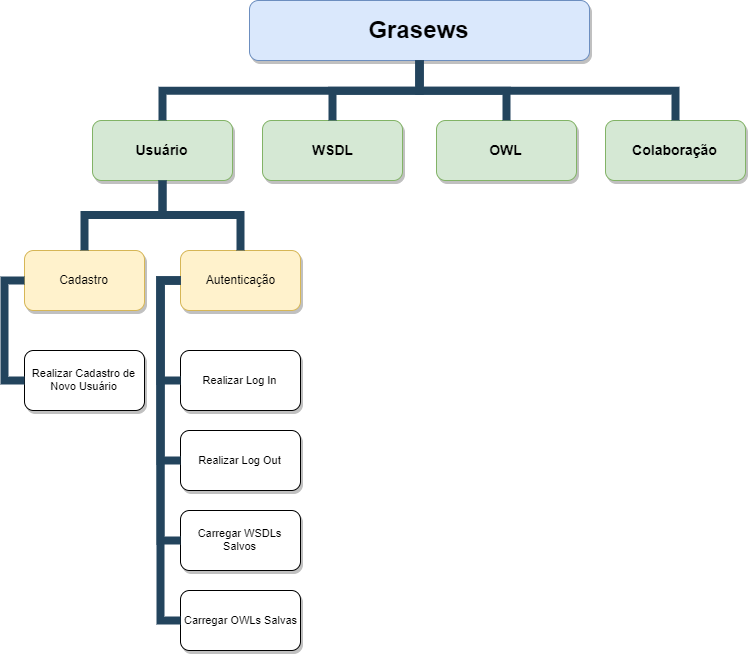
\includegraphics[scale=0.5]{9-pos-textuais/apendices/imagens/grasews-eap-usuario.png}
        %}
        \centering
        \caption[Estrutura Analítica de Projetos de Grasews - Parte 1]{\textbf{Estrutura Analítica de Projetos de Grasews - Parte 1.}}
        \label{fig:grasews-eap-usuario}
    \end{figure}
%\end{landscape}

%\begin{landscape}
    \begin{figure}[h]
        %\resizebox{\textwidth}{!}{
            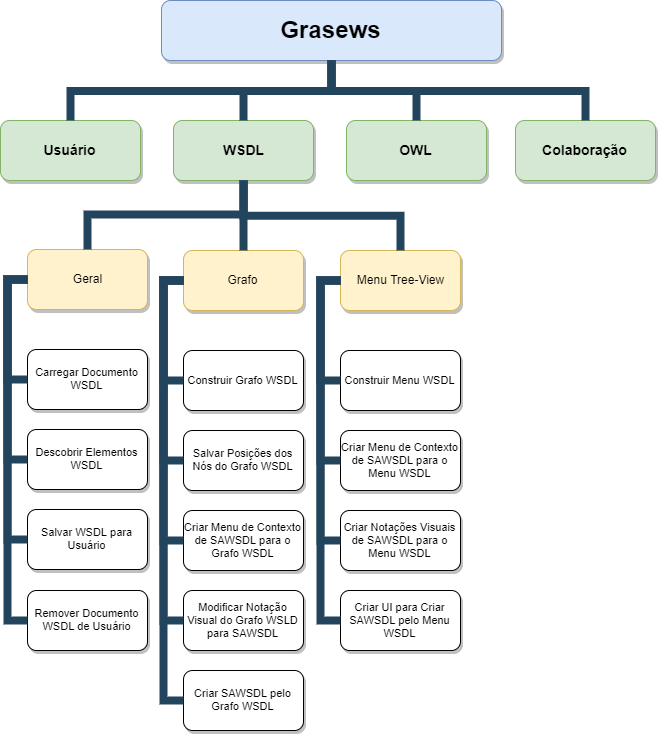
\includegraphics[scale=0.45]{9-pos-textuais/apendices/imagens/grasews-eap-wsdl.png}
        %}
        \centering
        \caption[Estrutura Analítica de Projetos de Grasews - Parte 2]{\textbf{Estrutura Analítica de Projetos de Grasews - Parte 2.}}
        \label{fig:grasews-eap-wsdl}
    \end{figure}
%\end{landscape}

%\begin{landscape}
    \begin{figure}[h]
        %\resizebox{\textwidth}{!}{
            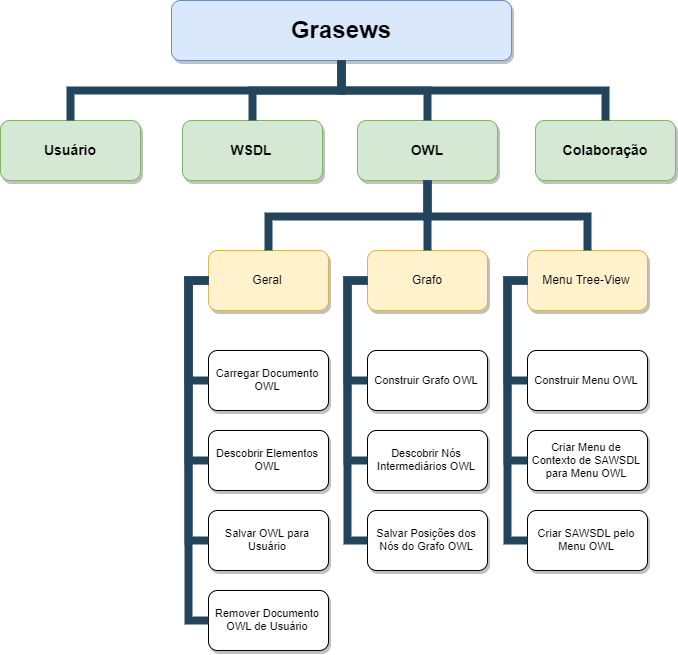
\includegraphics[scale=0.45]{9-pos-textuais/apendices/imagens/grasews-eap-owl.png}
        %}
        \centering
        \caption[Estrutura Analítica de Projetos de Grasews - Parte 3]{\textbf{Estrutura Analítica de Projetos de Grasews - Parte 3.}}
        \label{fig:grasews-eap-owl}
    \end{figure}
%\end{landscape}

%\begin{landscape}
    \begin{figure}[h]
        \resizebox{\textwidth}{!}{
            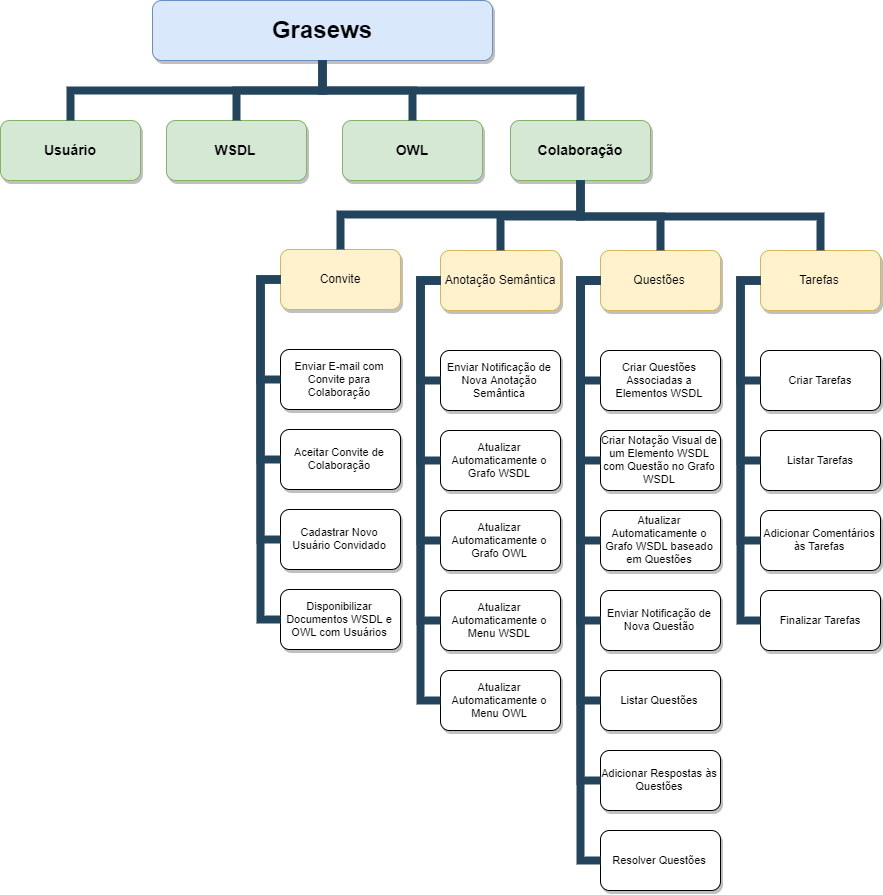
\includegraphics[scale=1]{9-pos-textuais/apendices/imagens/grasews-eap-colaboracao.png}
        }
        \centering
        \caption[Estrutura Analítica de Projetos de Grasews - Parte 4]{\textbf{Estrutura Analítica de Projetos de Grasews - Parte 4.}}
        \label{fig:grasews-eap-colaboracao}
    \end{figure}
%\end{landscape}
%\chapter{Questionário de Avaliação da ferramenta Grasews}\label{apendice-questionario-grasews}

\section{Questionário}

\begin{enumerate}[label=Q\arabic*]

    \item
    \textbf{Quão fácil foi a visualização de descrições de serviços web utilizando o Grasews?}
    \\
    ( ) Muito difícil ( ) Difícil ( ) Indiferente ( ) Fácil ( ) Muito fácil
    
    \item
    \textbf{Quão fácil foi a visualização de conceitos de ontologias utilizando o Grasews?}
    \\
    ( ) Muito difícil ( ) Difícil ( ) Indiferente ( ) Fácil ( ) Muito fácil

    \item
    \textbf{Quão fácil foi a criação de anotações semânticas utilizando o Grasews?}
    \\
    ( ) Muito difícil ( ) Difícil ( ) Indiferente ( ) Fácil ( ) Muito fácil

    \item
    \textbf{Quão fácil foi a visualização de anotações semânticas utilizando o Grasews?}
    \\
    ( ) Muito difícil ( ) Difícil ( ) Indiferente ( ) Fácil ( ) Muito fácil

    \item
    \textbf{Quão fácil foi a realização de um trabalho colaborativo para a criação de serviços web semânticos utilizando o Grasews?}
    \\
    ( ) Muito difícil ( ) Difícil ( ) Indiferente ( ) Fácil ( ) Muito fácil
    
    \item
    \textbf{Se já utilizou outras ferramentas de suporte à anotação semântica, quão mais fácil foi a anotação semântica utilizando o Grasews em relação à(s) outra(s) ferramenta(s)?}
    \\
    ( ) N/A
    \\
    ( ) Muito mais difícil ( ) Mais difícil ( ) Indiferente ( ) Mais fácil ( ) Muito mais fácil
    
    \item
    \textbf{Você acredita que a adoção de serviços web semânticos poderia ser beneficiada se houvesse um suporte ferramental mais adequado?}
    \\
    ( ) Discordo plenamente ( ) Discordo parcialmente ( ) Não discordo e nem concordo
    \\
    ( ) Concordo parcialmente ( ) Concordo plenamente
    
    \item
    \textbf{Você acredita que o Grasews pode contribuir para uma maior adoção de serviços web semânticos?}
    \\
    ( ) Discordo plenamente ( ) Discordo parcialmente ( ) Não discordo e nem concordo
    \\
    ( ) Concordo parcialmente ( ) Concordo plenamente
    
    \item
    \textbf{De 1 (muito ruim) a 5 (muito bom), como você avalia o Grasews?}
    \\
    ( ) 1\hspace{1cm}( ) 2\hspace{1cm}( ) 3\hspace{1cm}( ) 4\hspace{1cm}( ) 5
    
    \item
    \textbf{Tem algum sugestão que possa contribuir com melhorias do Grasews?}
    \\
    ....................................................................................................................................
    \\
    ....................................................................................................................................
    \\
    ....................................................................................................................................
    \\
    ....................................................................................................................................
    \\
    ....................................................................................................................................
    \\
    ....................................................................................................................................
    \\
    ....................................................................................................................................
    \\
    ....................................................................................................................................
    \\
    ....................................................................................................................................
    \\
    ....................................................................................................................................
    \\
    ....................................................................................................................................
    \\
    ....................................................................................................................................
    \\
    ....................................................................................................................................
    \\
    ....................................................................................................................................
    \\
    ....................................................................................................................................
    \\
    ....................................................................................................................................
    \\
    ....................................................................................................................................
    \\
    ....................................................................................................................................
    \\
    ....................................................................................................................................
    \\
    ....................................................................................................................................
    
\end{enumerate}

\section{Resultados}

\section{Conclusão}
\chapter{Tecnologias e Bibliotecas de Desenvolvimento}\label{apendice-tecnologias-grasews}

As principais tecnologias utilizadas no desenvolvimento de Grasews incluem:

\begin{enumerate}

  \item \textbf{Microsoft .NET Framework}
  
  .NET \textit{framework}~\cite{MICROSOFT-2019-NET-FRAMEWORK} é um \textit{framework} de desenvolvimento provido pela \textit{Microsoft}. Todos os módulos e componentes da ferramenta Grasews foram desenvolvidas utilizando a linguagem de programação C\# da versão 4.7 do \textit{framework} .NET. Os tipos de projetos .NET variam entre \textit{Asp.NET MVC}, para o módulo \texttt{Grasews.Web}, \textit{Asp.Net Web API}, para o módulo \texttt{Grasews.API}, e \textit{Class Library}, para os demais módulos da ferramenta.
  
  %Para mais informações, consulte \href{https://dotnet.microsoft.com/download/dotnet-framework/net472}{https://dotnet.microsoft.com/download/dotnet-framework/net472}
  
  \item \textbf{Microsoft ASP.NET MVC}
  
  ASP.NET~\cite{MICROSOFT-2019-ASP-NET-MVC} fornece recursos tecnológicos baseados em padrões para criar \textit{websites} dinâmicos usando o padrão \textit{Model-View-Controller} (MVC). MVC é um padrão de projeto usado para desacoplar a interface do usuário (visualização), os dados (modelo) e a lógica de aplicativo (controlador). Esse padrão ajuda a alcançar a separação de responsabilidades de forma mais clara.
  
  Ao usar o padrão MVC para o desenvolvimento de sites, as solicitações são encaminhadas para um \textit{controller} responsável por trabalhar com um \textit{model} para executar ações e / ou recuperar dados. Um \textit{controller} escolhe a \textit{view} para exibir e fornece o modelo (\textit{model}) para a página. Por fim, uma \textit{view} renderiza a página final com base nos dados de um \textit{model}. O módulo \texttt{Grasews.Web} foi desenvolvido utilizando este recurso.
  
  %Para mais informações, consulte \href{https://dotnet.microsoft.com/apps/aspnet/mvc}{https://dotnet.microsoft.com/apps/aspnet/mvc}
  
  \item \textbf{Microsoft ASP.NET Web API}
  
  \textit{ASP.NET Web API}~\cite{MICROSOFT-2019-WEB-API} é o formato mais recente utilizado para o desenvolvimento de serviços web RESTful do \textit{framework} .NET. O módulo \textit{Grasews.API} foi desenvolvido utilizado este recurso.
  
  %Para mais informações, consulte \href{https://dotnet.microsoft.com/apps/aspnet/apis}{https://dotnet.microsoft.com/apps/aspnet/apis}
  
  \item \textbf{Microsoft .NET Entity Framework}
  
  \textit{Entity Framework}~\cite{MICROSOFT-2019-Entity-Framework} é um \textit{Object Relational Mapper} (ORM) que permite que desenvolvedores trabalhem com um banco de dados por meio de objetos (instâncias de classes). Isso elimina a necessidade da maior parte do código de acesso a dados que os desenvolvedores geralmente precisam escrever, como, por exemplo, sentenças SQL (\textit{queries}). O módulo \texttt{Grasews.Postgres} utiliza \textit{.NET Entity Framework} para o acesso a dados existentes no SGBD \textit{Postgres}.
  
  %Para mais informações, consulte \href{https://docs.microsoft.com/en-us/ef/}{https://docs.microsoft.com/en-us/ef/}
  
  \item \textbf{Simple Injector}
  
  \textit{Simple Injector}~\cite{SIMPLE-INJECTOR-2019} é uma biblioteca de injeção de dependência de código aberto para o \textit{framework} NET. O módulo \texttt{Grasews.IoC} é responsável por controlar as injeções de dependências, suportado pela biblioteca \textit{Simple Injector}.
  
  %Para mais informações, consulte \href{https://simpleinjector.org/}{https://simpleinjector.org/}
  
  \item \textbf{AutoMapper}
  
  \textit{AutoMapper}~\cite{AUTO-MAPPER-2019} é uma biblioteca criada para mapear um objeto para outro. Ao invés de criar um método responsável por mapear propriedades de um objeto para propriedades de outro objeto, uma a uma, \textit{AutoMapper} simplifica o código, deixando o trabalho mais simples para desenvolvedores de \textit{software} utilizando o \textit{framework} .NET. A biblioteca \textit{AutoMapper} é um recurso que provê o padrão de projeto \textit{Adapter}. \textit{AutoMapper} é utilizado na conversão entre objetos \texttt{Models} dos módulos \texttt{Grasews.Web} e \texttt{Grasews.API}, objetos \texttt{DTOs} do módulo \texttt{Grasews.Application} e entidades de domínio do módulo \texttt{Grasews.Domain}.
  
  %Para mais informações, consulte \href{https://automapper.org/}{https://automapper.org/}
  
  \item \textbf{OWIN}
  
  \textit{OWIN}~\cite{OWIN-2019} é uma uma interface padrão de desenvolvimento entre o lado servidor e o lado cliente de uma aplicação desenvolvida com o \textit{framework} .NET. \textit{OWIN} tem o propósito de desacoplar serviços do lado servidor e aplicativos Web desenvolvidos utilizando o \textit{framework} .NET, permitindo uma melhor comunicação entre os módulos \texttt{Grasews.Web} e \texttt{Grasews.API}.
  
  %Para mais informações, consulte \href{http://owin.org/}{http://owin.org/}
  
  \item \textbf{OAuth 2.0}
  
  \textit{OAuth} 2.0~\cite{OAUTH-2019} é o protocolo padrão para autorização de aplicações. \textit{OAuth} 2.0 fornece fluxos de autorização específicos para aplicativos da web, dispositivos móveis e computadores. Os módulos \texttt{Grasews.Web} e \texttt{Grasews.API} utilizam \textit{OAuth} 2.0 para o controle de autenticação e autorização de um usuário de Grasews.
  
  %Para mais informações, consulte \href{https://oauth.net/}{https://oauth.net/}
  
  \newpage
  
  \item \textbf{Microsoft ASP.NET Identity}
  
  \textit{Microsoft ASP.NET Identity}~\cite{MICROSOFT-2019-IDENTITY} é uma biblioteca de desenvolvimento do \textit{framework} .NET que provê suporte a controles de segurança de uma aplicação. Por meio de \textit{Microsoft ASP.NET Identity}, Grasews possui integração com o protocolo \textit{OAuth} e a interface \textit{OWIN}. Os módulos \texttt{Grasews.Web}, \texttt{Grasews.API} e \texttt{Grasews.Security} utilizam a biblioteca \textit{Microsoft ASP.NET Identity}.
  
  %Para mais informações, consulte \href{https://docs.microsoft.com/en-us/aspnet/identity/}{https://docs.microsoft.com/en-us/aspnet/identity/}
  
  \item \textbf{Postgres}
  
  \textit{PostgreSQL}~\cite{POSTGRES-2019} é um sistema banco de dados relacional de objetos de código aberto. O módulo \texttt{Grasews.Infra.Data.EF.Postgres} utiliza bibliotecas de desenvolvimento que proveem conectividade entre \textit{Entity Framework} e \textit{Postgres}.
  
  %Para mais informações, consulte \href{https://www.postgresql.org/}{https://www.postgresql.org/}
  
  \item \textbf{Sentry}
  
  \textit{Sentry}~\cite{SENTRY-2019} fornece uma plataforma de monitoramento de erros baseada na nuvem. \textit{Sentry} possui um conjunto de bibliotecas disponíveis para o \textit{framework} .NET e outras linguagens o qual torna possível capturar erros de uma aplicação e enviar as especificações dos erros para a ferramenta da web. Por meio da ferramenta da web de \textit{Sentry}, o monitoramento e gerenciamento de erros é facilitado. Equipes de desenvolvimento podem mais facilmente descobrir, fazer triagem e priorizar erros em tempo real. Todos os módulos de Grasews utilizam \textit{Sentry} para a captura de exceções.
  
  %Para mais informações, consulte \href{https://sentry.io/}{https://sentry.io/}
  
  \item \textbf{Cytoscape.js}
  
  \textit{Cytoscape.js}~\cite{CYTOSCAPE-2015} é uma biblioteca \textit{JavaScript} para a visualização e análise de grafos. O módulo \texttt{Grasews.Web} utiliza esta biblioteca para a criacão do grafo na interface de usuário. Adicionalmente, o módulo \texttt{Grasews.Cytoscape} é responsável por manipular e construir objetos (modelos), por meio da linguagem de programação C\#, utilizados pela biblioteca \textit{Cytoscape.js}
  
  %Para mais informações, consulte \href{http://js.cytoscape.org/}{http://js.cytoscape.org/}
  
  \item \textbf{Admin LTE}
  
  \textit{Admin LTE}~\cite{ADMIN-LTE-2019} é um modelo de interface de usuário utilizado para a construção de painéis de administração. \textit{Admin LTE} possui o código aberto e disponibiliza diversas variações, customizações e tema de painel de controle. \textit{Admin LTE} fornece uma variedade de componentes responsivos, reutilizáveis e comumente usados em sistemas web. \textit{Admin LTE} é construído sobre o \textit{Bootstrap}. O módulo \texttt{Grasews.Web} utiliza \textit{Admin LTE} em sua interface gráfica de usuário.
  
  %Para mais informações, consulte \href{https://adminlte.io/}{https://adminlte.io/}
  
  \newpage
  
  \item \textbf{Bootstrap}
  
  \textit{Bootstrap}~\cite{BOOTSTRAP-2019} é uma biblioteca de código aberto para o desenvolvimento de aplicações web com HTML, CSS e \textit{JavaScript}. \textit{Bootstrap} fornece um conjunto de componentes responsivos para diversos dispositivos, além de um sistema de grade responsivo, extensos componentes pré-construídos e \textit{plugins} criados no \textit{jQuery}. O módulo \texttt{Grasews.Web} utiliza \textit{Bootstrap}, em conjunto com \textit{Admin LTE} na implementação da interface gráfica de usuário.
  
  %Para mais informações, consulte \href{https://getbootstrap.com/}{https://getbootstrap.com/}

  \item \textbf{jQuery}
  
  \textit{jQuery}~\cite{JQUERY-2019} é uma biblioteca \textit{JavaScript} que simplifica a manipulação de documentos HTML, a manipulação de eventos, animações e o gerenciamento de requisições AJAX. O módulo \texttt{Grasews.Web} utiliza \textit{jQuery} para a construção de funcionalidades da interface gráfica de usuário de Grasews.
  
  %Para mais informações, consulte \href{https://jquery.com/}{https://jquery.com/}
  
  \item \textbf{Font-Awesome}
  
  \textit{Font-Awesome}~\cite{FONT-AWESOME-2019} é uma biblioteca de ícones vetoriais e escaláveis que podem ser personalizados instantaneamente. Tamanho, cor, sombreamento e outras propriedades dos ícones podem ser facilmente modificadas por meio de CSS. O módulo \texttt{Grasews.Web} utiliza ícones providos pela versão 4.7 de \textit{Font-Awesome} para a construção da interface gráfica de usuário de Grasews.
  
  %Para mais informações, consulte \href{https://fontawesome.com/v4.7.0/}{https://fontawesome.com/v4.7.0/}
  
  \item \textbf{CodeMirror}
  
  \textit{CodeMirror}~\cite{CODEMIRROR-2019} é um editor de texto implementado utilizando a linguagem \textit{JavaScript}. \textit{CodeMirror} possui vários modos que dão suporte a manipulação de diversas linguagens de programação. Adicionalmente, \textit{CodeMirror} possui um conjunto de temas CSS que possibilitam customizar o editor de texto. O módulo \texttt{Grasews.Web} utiliza a biblioteca \textit{CodeMirror} no painel de exibição do código WSDL de uma descrição de serviço web na interface gráfica de usuário de Grasews.
  
  %Para mais informações, consulte \href{https://codemirror.net/}{https://codemirror.net/}
  
  \item \textbf{Microsoft SignalR}
  
  \textit{Microsoft SignalR}~\cite{MICROSOFT-2019-SIGNALR} é parte do \textit{framework} .NET que tem como foco a implementação de \textit{web-sockets}. Por meio de \textit{Microsoft SignalR}, aplicações web desenvolvidas em .NET (lado cliente) podem receber atualizações do lado servidor de forma passiva. \textit{Microsoft SignalR} implementa o padrão de projeto \textit{Observer}. Com isso, o lado cliente permanece observando mensagens que são registradas no lado servidor por meio de canais de comunicação denominados \textit{hubs}. Quando uma nova mensagem é registrada em um \textit{hubs}, o lado cliente responde à essa mensagem. \textit{Microsoft SignalR} permite que o módulo \texttt{Grasews.Web} atualize os ambientes de trabalho dos usuários que estão trabalhando de forma colaborativa em uma especificação WSDL aberta na ferramenta. Adicionalmente, além das atualizações dos ambientes de trabalho, os usuários recebem notificações informando-os sobre novas atualizações em uma dada especificação WSDL.
  
  %Para mais informações, consulte \href{https://dotnet.microsoft.com/apps/aspnet/signalr}{https://dotnet.microsoft.com/apps/aspnet/signalr}
  
  \item \textbf{Swagger OpenAPI Specification}
  
  Swagger~\cite{SMARTBEAR-2019-SWAGGER} é uma estrutura de software de código aberto que apoia desenvolvedores a projetar, criar, documentar e consumir serviços da Web RESTful. O módulo \texttt{Grasews.API} provê uma documentação web (\textit{help pages}) com a descrição de suas funcionalidades web por meio do formato \textit{OpenAPI}, automaticamente criado pelo \textit{framework} .NET.
  
  %Para mais informações, consulte \href{https://swagger.io/}{https://swagger.io/}
  
  \item \textbf{JSON}
  
  \textit{JavaScript Object Notation} (JSON)~\cite{JSON-2019} é um formato padrão para troca de dados. JSON é de fácil compreensão tanto para humanos quanto para máquinas. Este formato é completamente independente de linguagens de programação. Toda comunicação realizada entre os módulos \texttt{Grasews.Web} e \texttt{Grasews.API} é realizada por meio de mensagens no formato JSON. Adicionalmente, a construção do grafo por meio da biblioteca \textit{Cytoscape.js} também é feita por meio de objetos no formato JSON.
  
\end{enumerate}



\end{apendicesenv} % descomentar
%\begin{anexosenv}

% Imprime uma página indicando o início dos anexos
\partanexos

\chapter{Artefatos da Prova de Conceito}\label{anexo-artefatos-estudo-de-caso}

\section{Especificação WSDL original}\label{anexo-WSDL-estudo-de-caso}

A \lstlistingname~\ref{lst:estudo-de-caso-wsdl} apresenta o código da especificação WSDL original utilizado pelo estudo de caso no Capítulo \ref{5-estudo-de-caso} deste trabalho. Note que não há anotação semântica alguma e nem a existência do \textit{namespace} de SAWSDL.

\lstinputlisting[language=xml,caption={[Especificação WSDL do estudo de caso]\textbf{Especificação WSDL do estudo de caso}.},label={lst:estudo-de-caso-wsdl}]{9-pos-textuais/anexos/arquivos/movie-original.wsdl}

%\section{Ontologia OWL}\label{anexo-OWL-estudo-de-caso}

%A \lstlistingname~\ref{lst:estudo-de-caso-wsdl-anotado} apresenta o código da especificação WSDL após a anotação semântica realizada pelo estudo de caso no Capítulo \ref{5-estudo-de-caso} deste trabalho.

%\lstinputlisting[language=xml,caption={[Ontologia OWL do estudo de caso]\textbf{Ontologia OWL do estudo de caso}.},label={lst:estudo-de-caso-owl}]{pos-textuais/anexos/arquivos/movieontology.owl}

\section{Especificação WSDL com Anotação Semântica}\label{anexo-WSDL-anotado-estudo-de-caso}

A \lstlistingname~\ref{lst:estudo-de-caso-wsdl-anotado} apresenta o código da especificação WSDL após a anotação semântica realizada pelo estudo de caso no Capítulo \ref{5-estudo-de-caso} deste trabalho.

\lstinputlisting[language=xml,caption={[Especificação WSDL anotada após o estudo de caso]\textbf{Especificação WSDL anotada após o estudo de caso}.},label={lst:estudo-de-caso-wsdl-anotado}]{9-pos-textuais/anexos/arquivos/movie-anotado.wsdl}

\end{anexosenv} % descomentar

%---------------------------------------------------------------------
% INDICE REMISSIVO
%---------------------------------------------------------------------
\phantompart
\printindex
%---------------------------------------------------------------------

\end{document}